%%%%%%%%%%%%%%%%%%%%%%% file template.tex %%%%%%%%%%%%%%%%%%%%%%%%%
%
% This is a template file for the global option of the SVJour class
%
% Copy it to a new file with a new name and use it as the basis
% for your article
%
%%%%%%%%%%%%%%%%%%%%%%%% Springer-Verlag %%%%%%%%%%%%%%%%%%%%%%%%%%
%
%% First comes an example EPS file -- just ignore it and
%% proceed on the \documentclass line
%\begin{filecontents*}{example.eps}
%%!PS-Adobe-3.0 EPSF-3.0
%%%BoundingBox: 19 19 221 221
%%%CreationDate: Mon Sep 29 1997
%%%Creator: programmed by hand (JK)
%%%EndComments
%gsave
%newpath
%  20 20 moveto
%  20 220 lineto
%  220 220 lineto
%  220 20 lineto
%closepath
%2 setlinewidth
%gsave
%  .4 setgray fill
%grestore
%stroke
%grestore
%\end{filecontents*}
%
% Choose either the first of the next two \documentclass lines for one
% column journals or the second for two column journals.
%\documentclass[global,referee]{svjour}
\documentclass[global,twocolumn]{svjour}
%\documentclass[global,twocolumn,referee]{svjour}
% Remove option referee for final version
%
% Remove any % below to load the required packages
%\usepackage{latexsym}

\usepackage{lscape}
\usepackage{pdflscape}
\usepackage{amsmath}
\usepackage{float}
\usepackage[utf8]{inputenc}
\usepackage[T1]{fontenc}
\usepackage{lmodern}
\usepackage{microtype} % optional, for aesthetics
\usepackage{tabularx} % nice to have
\usepackage{booktabs}
\usepackage{makecell}
\usepackage{cite}
\usepackage{hhline}
\usepackage{parskip}
\usepackage{wrapfig}
\usepackage{lscape}
\usepackage{xcolor}
\usepackage{ragged2e}
\usepackage{enumitem}
\usepackage{graphicx}
\usepackage{booktabs}
\setlist[enumerate]{label*=\arabic*.}
\usepackage{makecell}
\usepackage{kantlipsum}
\usepackage{enumitem}
\usepackage{tabularx}
\usepackage{appendix}
\usepackage{hhline}
\usepackage{array}
\usepackage{subcaption}
%\usepackage{caption}
\graphicspath{{figures/}} 
\usepackage{multirow}
\usepackage{hyperref}
\hypersetup{colorlinks=true,allcolors=blue}
\usepackage{hypcap}
\usepackage{courier}
\usepackage[linesnumbered,ruled]{algorithm2e}
\usepackage{algcompatible}
\usepackage{listings}
\lstset{
basicstyle=\ttfamily,
frame=none, 
breaklines=true,
numbers=left,
xleftmargin=2.5em,
framexleftmargin=0em,
emphstyle=\textbf,
float=t
}
\lstdefinestyle{ocl}{
basicstyle=\ttfamily\scriptsize,
emph={
context, inv
}
}
\lstdefinestyle{cbpfile}{
basicstyle=\ttfamily\scriptsize,
emph={
session, register, create, delete, add, resource,
set eattribute, epackage, eclass, value, old,
position, from, to, unset, ereference, unset, eattribute,
move, in, ereference, eobject, literal,
remove, composite, time, id
}
}
\lstdefinestyle{xmi}{
basicstyle=\ttfamily\scriptsize,
emph={
Node, children
}
}
\lstdefinestyle{xml}{
basicstyle=\ttfamily\scriptsize,
emph={
register, create, add, to, resource, at,
from, eattribute, remove, ereference,
set, unset, session, Roy, Jen,
Moss, Richmond
}
}
\lstdefinestyle{java}{
basicstyle=\ttfamily\scriptsize,
emph={
case, $unset$,
instanceof, else, if, void,
new, UnsetEAttributeEvent,
UnsetEReferenceEvent,
@override, public, class, extends
}
}
\lstdefinestyle{eol}{
basicstyle=\ttfamily\scriptsize,
emph={
var, new, for, in, create, set, with, type, at,
unset, to, add, remove, delete, register, move,
composite,
from, position, from, move-within, session, \.
}
}

\hyphenation{op-tical net-works semi-conduc-tor Hybrid-Change-Event-Adapter Hybrid-XMI-Change-Event-Adapter
Hybrid-Neo-EMF-Change-Event-Adapter change-events Change-Event-Adapter EContent-Adapter notify-Changed Hybrid-Resource Resource-Impl state-Based-Resource cbp-Output-Stream Output-Stream Hybrid-Change-Event-Adapter Output-Stream Hybrid-XMI-Resource-Impl Hybrid-Neo-EMF-Resource-Impl Persistence-Resource change-Events get-All-Re-la-ted-Left-E-vents get-All-Re-la-ted-Right-E-vents get-Unequal-Left-And-Right-Values get-Unequal-Left-And-Right-Values get-XOR-Left-And-Right-Values
}

\definecolor{gray1}{gray}{0.90}
\definecolor{gray2}{gray}{0.95}

%\renewcommand{\thelstlisting}{\arabic{lstlisting}}
\renewcommand{\labelitemi}{$\bullet$}
\newcommand{\AndA}{\textnormal{\textbf{and }}}
\newcommand{\Is}{\textnormal{\textbf{is }}}
\newcommand{\Not}{\textnormal{\textbf{not }}}
\newcommand{\In}{\textnormal{\textbf{in }}}
\newcommand{\Or}{\textnormal{\textbf{or }}}
\newcommand{\eqnum}{\refstepcounter{equation}\textup{\tagform@{\theequation}}}

% etc
%
% Insert the name of "your" journal with the command below:
\journalname{myjournal}
%
\begin{document}
%
\title{Towards Efficient Conflict Detection of Change-Based Models}
%\subtitle{Do you have a subtitle?\\ If so, write it here}
\author{Alfa Yohannis\inst{1,2} 
%	\and Horacio Hoyos Rodriguez\inst{1} 
%	\and Fiona Polack\inst{3} 
	\and Dimitris Kolovos\inst{1}% etc
% \thanks is optional - remove next line if not needed
%\thanks{\emph{Present address:} Insert the address here if needed}%
}                     % Do not remove
%
\offprints{}          % Insert a name or remove this line
%
\institute{Department of Computer Science, University of York, United Kingdom  
\and Department of Informatics, Kalbis Institute, Indonesia
%\and School of Computing and Maths, Keele University, United Kingdom
}
%
\date{Received: 1 December 2021 / Revised version: 31 December 2021}
% The correct dates will be entered by the editor
%
\maketitle
%
\begin{abstract}
Using traditional state-based modelling tools, model management of large models is time-consuming, resulting in model operations, such as conflict detection, suffering significant bottlenecks in collaborative modelling environments. For example, 3-way, state-based model conflict detection requires loading three versions of a model, deriving changes by differencing two versions with their common ancestor, and checking if the changes conflict. This paper presents our change-based persistence approach, which relies on storing changes from a base model rather than all model versions. We show how change-based persistence supports efficient model conflict detection. We summarise performance results, with conflict detection time is reduced in some experiments, compared to traditional state-based model conflict detection.
\end{abstract}
%

\section{Introduction}
\label{sec:introduction}

In the context of model-driven engineering processes, models are commonly persisted in state-based formats. In such approaches, model files contain snapshots of the models' contents, and activities like version control and change detection are left to external systems such as file-based version-control systems and model differencing facilities. Activities such as model differencing (identifying parts of two versions of a model that are different) and conflict detection (finding conflicting changes between two versions of a model) are computationally expensive for state-based models \cite{Kolovos:2009:DMM:1564596.1564641} since every element has to be inspected, matched to its respective pair, compared to identify their differences, and checked whether changes in the different versions are inconsistent \cite{emfcompare2018developer}. Element-wise differencing in state-based model versions is inefficient because, in most cases, only a few elements are changed between versions. The inefficiency is most significant in large models and where mature modules are subject to fine-tuning by different collaborators \cite{selic2003pragmatics}. 

As an alternative to state-based persistence, models can be persisted in a change-based format that records the full sequence of changes made rather than the model itself. The concept of change-based persistence is not new and has been used to persist changes to software, object-oriented databases, and hierarchical documents \cite{DBLP:journals/entcs/RobbesL07,DBLP:conf/sde/LippeO92,DBLP:conf/caise/IgnatN05}. The change-based approach can improve detecting differences more precisely at the semantic level by providing finer-granularity information (e.g. types of changes, the order of the changes, 
elements that were changed, previous values, etc.) and better support to resolve them \cite{mens2002state}. The ordered nature of change-based persistence also means that changes made to a model since its previous version can be identified sequentially without inspecting every element of the model and comparing it to its previous version. 
In terms of performance, our previous study \cite{yohannis2019efficient} has found that using a change-based approach, we can perform model differencing faster than its state-based counterpart. Furthermore, since state-based conflict detection also employs a state-based model differencing to identify model changes, we expect the change-based approach to perform better than the state-based approach in detecting conflicts. Based on these arguments, this research to answer the following research question, \textbf{``How and to what extent does change-based model persistence speed up the detection of model conflict, and with what effects on the memory footprint, compared to state-based model conflict detection?''}. 

\begin{figure*}[]
\centering
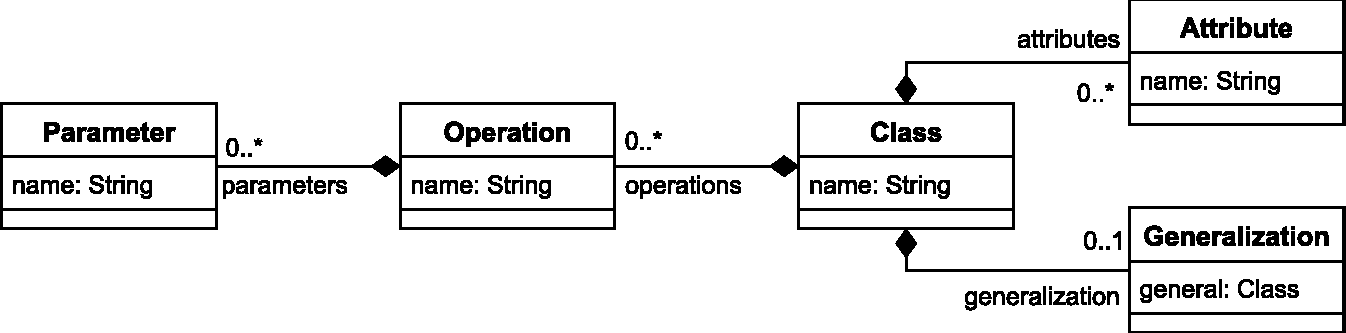
\includegraphics[width=0.7\linewidth]{miniuml_metamodel}
\caption{An excerpt of the UML-like metamodel of the running example in Figure \ref{fig:class_diagram_rpg}.}
\label{fig:miniuml_metamodel}
\end{figure*}

\begin{figure*}[]
\centering
\begin{subfigure}[t]{0.31\linewidth}
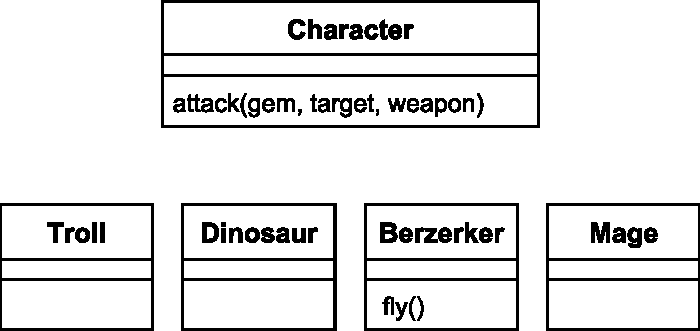
\includegraphics[width=\linewidth]{class_diagram_origin}
\caption{original version (Jane's version)}
\label{fig:class_diagram_origin}
\end{subfigure}
\hfill
\begin{subfigure}[t]{0.31\linewidth}
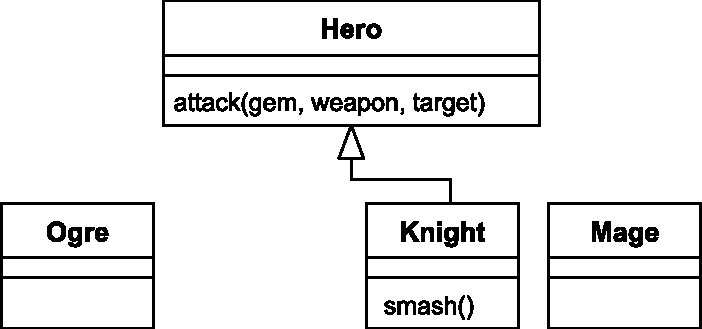
\includegraphics[width=\linewidth]{class_diagram_left}
\caption{left version (Bob's version)}
\label{fig:class_diagram_left}
\end{subfigure}
\hfill
\begin{subfigure}[t]{0.31\linewidth}
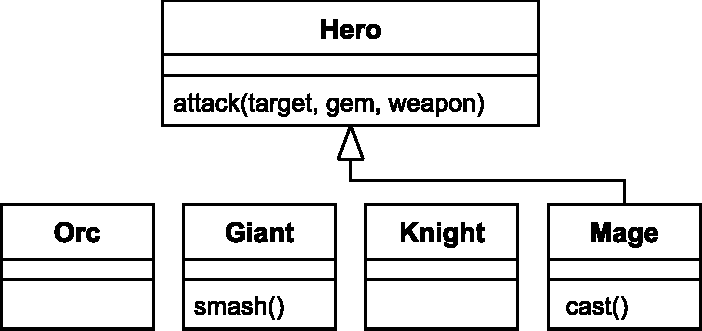
\includegraphics[width=\linewidth]{class_diagram_right}
\caption{right version (Alice's version)}
\label{fig:class_diagram_right}
\end{subfigure}
\caption{Three incomplete class diagrams of a Role Playing Game.}
\label{fig:class_diagram_rpg}
\end{figure*}

To address the question, our work has been able to build an implementation of a change-based persistence format for Eclipse Modeling Framework (EMF) \cite{eclipse2019emf} and has used it to speed up model conflict detection. The implementation of the change-based model persistence format, the approach that leverages it to speed up model conflict detection as well as its evaluation are presented in this paper. 

This paper summarises our approach to change-based persistence, extending our work presented in \cite{DBLP:conf/models/YohannisKP17} (an initial implementation) and \cite{yohannis2019efficient} (using change-based-persistence for model differencing). In this paper, we extend both work \cite{DBLP:conf/models/YohannisKP17,yohannis2019efficient} by reporting on the use of change-based model persistence to speed up model conflict detection. This paper is structured as follows. Section \ref{sec:running_example} introduces a running example that is used throughout this paper to explain our proposed approach. Section \ref{sec:emf_change_based_persistence} briefly describes the design and implementation of our change-based model persistence approach.  
Section \ref{sec:existing_conflict_detections} discusses how state-of-the-art tools such as, EMF Compare and EMF Store, perform conflict detection. 
Section \ref{sec:emf_cbp_conflict_detection} describes in detail how our approach exploits change-based model persistence to speed up model conflict detection. Sections \ref{sec:conflict_algorithm_complexity} and \ref{sec:accuracy_of_conflict_detection} discuss the algorithm complexity and accuracy of conflict detection. 
Section \ref{sec:evaluation_method} describes how we evaluated our approach, and Section \ref{sec:evaluation_discussion} discusses the results of the evaluation. Section \ref{sec:related_work} presents related work of this study. Finally, Section \ref{sec:conclusions_and_future_work} concludes and discusses future work.

\section{Running Example}
\label{sec:running_example}

Before going deeper into change-based persistence and discussing future work, this paper introduces a running example. Figure \ref{fig:class_diagram_rpg} shows three versions of an incomplete model conforming to a simplified UML-like metamodel in Figure \ref{fig:miniuml_metamodel}. The metamodel is minimalist only to facilitate explaining the running example. This example is used throughout this paper to explain the solutions proposed and how conflict detection is performed in the related work, such as in EMF Compare \cite{emfcompare2018developer} and EMF Store \cite{emfstore2019what}. 

In our scenario, Jane has set up the initial model of a Role Playing Game (RPG) (Figure \ref{fig:class_diagram_origin}). She then assigned this work to Bob and Alice. Both of Alice and Bob continued to work on the model and made some modifications producing the models in Figures \ref{fig:class_diagram_left} and \ref{fig:class_diagram_right} respectively. Persisting these models in the standard XMI \cite{omg2018xmi} format produces three files as shown in Listings \ref{lst:xmimodel_origin}, \ref{lst:xmimodel_left}, and \ref{lst:xmimodel_right}. In this running example, every element has its globally unique id. Thus, if Bob and Alice create two elements independently, they will not be allocated the same id. For example, the generalizations that Bob and Alice added in Listings \ref{lst:xmimodel_left} and \ref{lst:xmimodel_right} have different ids, \textsf{leftGen} and \textsf{rightGen} respectively.  
\begin{lstlisting}[style=xmi,caption={Simplified XMI file of the original version in Figure \ref{fig:class_diagram_origin}.},label=lst:xmimodel_origin]
<uml:Model>
<packagedElement type=Class id="character" name="Character">
<operation id="attack" name="attack">
<parameter id="gem" name="gem"/>
<parameter id="target" name="target"/>
<parameter id="weapon" name="weapon"/>
</operation>
</packagedElement>
<packagedElement type=Class id="troll" name="Troll"/>
<packagedElement type=Class id="giant" name="Giant">
<operation id="cast" name="cast"/>
</packagedElement>
<packagedElement type=Class id="knight" name="Knight">
<operation id="smash" name="smash"/>
</packagedElement>
<packagedElement type=Class id="mage" name="Mage"/>
</uml:Model>
\end{lstlisting}

\begin{lstlisting}[style=xmi,caption={Simplified XMI file of the left version in Figure \ref{fig:class_diagram_left}.},label=lst:xmimodel_left]
<uml:Model>
<packagedElement type=Class id="character" name="Hero">
<operation id="attack" name="attack">
<parameter id="weapon" name="weapon"/>
<parameter id="gem" name="gem"/>
<parameter id="target" name="target"/>
</operation>  
</packagedElement>
<packagedElement type=Class id="troll" name="Ogre"/>
<packagedElement type=Class id="knight" name="Knight">
<generalization id="leftGen" general="character"/>
<operation id="smash" name="smash"/>
</packagedElement>
<packagedElement type=Class id="mage" name="Mage"/>
</uml:Model>
\end{lstlisting}

\begin{lstlisting}[style=xmi,caption={Simplified XMI file of the right version of Figure \ref{fig:class_diagram_right}.},label=lst:xmimodel_right]
<uml:Model>
<packagedElement type=Class id="character" name="Character">
<operation id="attack" name="attack">
<parameter id="gem" name="gem"/>
<parameter id="weapon" name="weapon"/>
<parameter id="target" name="target"/>
</operation>
</packagedElement>
<packagedElement type=Class id="troll" name="Orc"/>
<packagedElement type=Class id="giant" name="Giant">
<operation id="smash" name="smash"/>
</packagedElement>
<packagedElement type=Class id="knight" name="Knight"/>
<packagedElement type=Class id="mage" name="Mage">
<generalization id="rightGen" general="character"/>
<operation id="cast" name="cast"/>
</packagedElement>
</uml:Model>
\end{lstlisting}

An alternative way of persisting these three models would be to persist, instead of their state, the sequence of all changes through which they were constructed. This approach was first introduced in \cite{DBLP:conf/models/YohannisKP17} and is illustrated in the next section.


\section{EMF Change-Based Persistence}
\label{sec:emf_change_based_persistence}

To illustrate the proposed approach, Listing \ref{lst:xmimodel_left} shows a state-based representation of the model of Figure \ref{fig:class_diagram_left} in (simplified) XMI, and Listing \ref{lst:cbp_left_full} shows the proposed equivalent change-based representation of the same model. Instead of persisting a snapshot of the model's state, the representation of Listing \ref{lst:cbp_left_full} captures the complete sequence of change events (create/set/add/move/remove/delete) that were performed on the model since its creation, organised in editing sessions. There are two editing session in the case of this model: session at line 1 marks the editing made by Jane until line 29. Replaying these changes produces Jane's model in Figure \ref{fig:class_diagram_origin}. The rest of the change events are the modification performed by Bob on Jane's model. Replaying all the changes, all Jane's and Bob's changes, produces the same state as the one captured in Listing \ref{lst:xmimodel_left} or Figure \ref{fig:class_diagram_left}. Thus, we can conclude that the proposed change-based representation carries at least as much information as the state-based representation. 

\begin{lstlisting}[style=eol,escapechar=|,caption={The complete change events of Bob's model in Figure \ref{fig:class_diagram_left}.},label=lst:cbp_left_full]
session "Jane-01"
create character type Class
set character.name from null to "Character" 
create attack type Operation
set attack.name from null to "attack" 
add attack to character.operations at 0
create gem type Parameter
set gem.name from null to "gem" 
add gem to attack.parameters at 0
create target type Parameter
set target.name from null to "target" 
add target to attack.parameters at 1
create weapon type Parameter
set weapon.name from null to "weapon" 
add weapon to attack.parameters at 2
create troll type Class
set troll.name from null to "Troll" 
create giant type class
set giant.name from null to "Giant"
create cast type Operation
set cast.name from null to "smash"
add cast to giant.operations at 0
create knight type Class
set knight.name from null to "Knight"
create smash type Operation
set smash.name from null to "smash"
add smash to knight.operations at 0
create mage type Class
set mage.name from null to "Mage" 
session "Bob-01"
create leftGen type Generalization
set leftGen.general from null to character
set troll.generalization to leftGen
set character.name from "Character" to "Hero"
unset troll.generalization from leftGen to null composite l1
set knight.generalization to leftGen composite l1
move target in attack.parameters from 1 to 2
unset cast.name from "cast" to null composite l2
remove cast from giant.operations at 0 composite l2
delete cast composite l2
unset giant.name from "Giant" to null composite l2
delete giant composite l2
set troll.name from "Troll" to "Ogre"
\end{lstlisting}

Such a representation is particularly suitable to identify recent changes of the model since the last version. For example, if we can identify that changes recorded for the previous version are up to the right before the editing session \textsf{Bob-01} (lines 1-29) of the model, it can readily identify the changes that have been made to the model since then (i.e. in session \textsf{Bob-01} -- lines 30-43) instead of having to rediscover them through expensive state-based model differencing.

For the sake of readability, the format of change-based persistence presented in Listing \ref{lst:cbp_left_full} is a simplified version. The real format is in XML-like-format. For example, change event \textsf{session "Jane-01"} is persisted as:

\textsf{<session id="Jane-01" time="20190923181841687GMT"/>} 

and \textsf{set character.name from null to "Character"} is persisted as:

\textsf{<set-eattribute eclass="Class" name="name" 
target = "character">
<old-value literal=null/>
<value literal = "Character"/>
</set-eattribute>}.

Change events that have been persisted to a change-based persistence file cannot be altered or removed – immutable,  only new change events that can be appended to the file.

\subsection{Prototype Implementation}
\label{sec:prototype_implementation}

A prototype \cite{epsilonlabs2019emfcbp} of the change-based model persistence format (EMF CBP) has been implemented using the model-element level change notification facilities provided by the Eclipse Modelling Framework. In the implementation, the prototype uses a subclass of EMF's \textsf{EContentAdapter} (\textsf{ChangeEventAdapter}) to receive and record \textsf{Notification} events produced by the framework for every model-element level change.

\begin{figure*}[th]
\centering
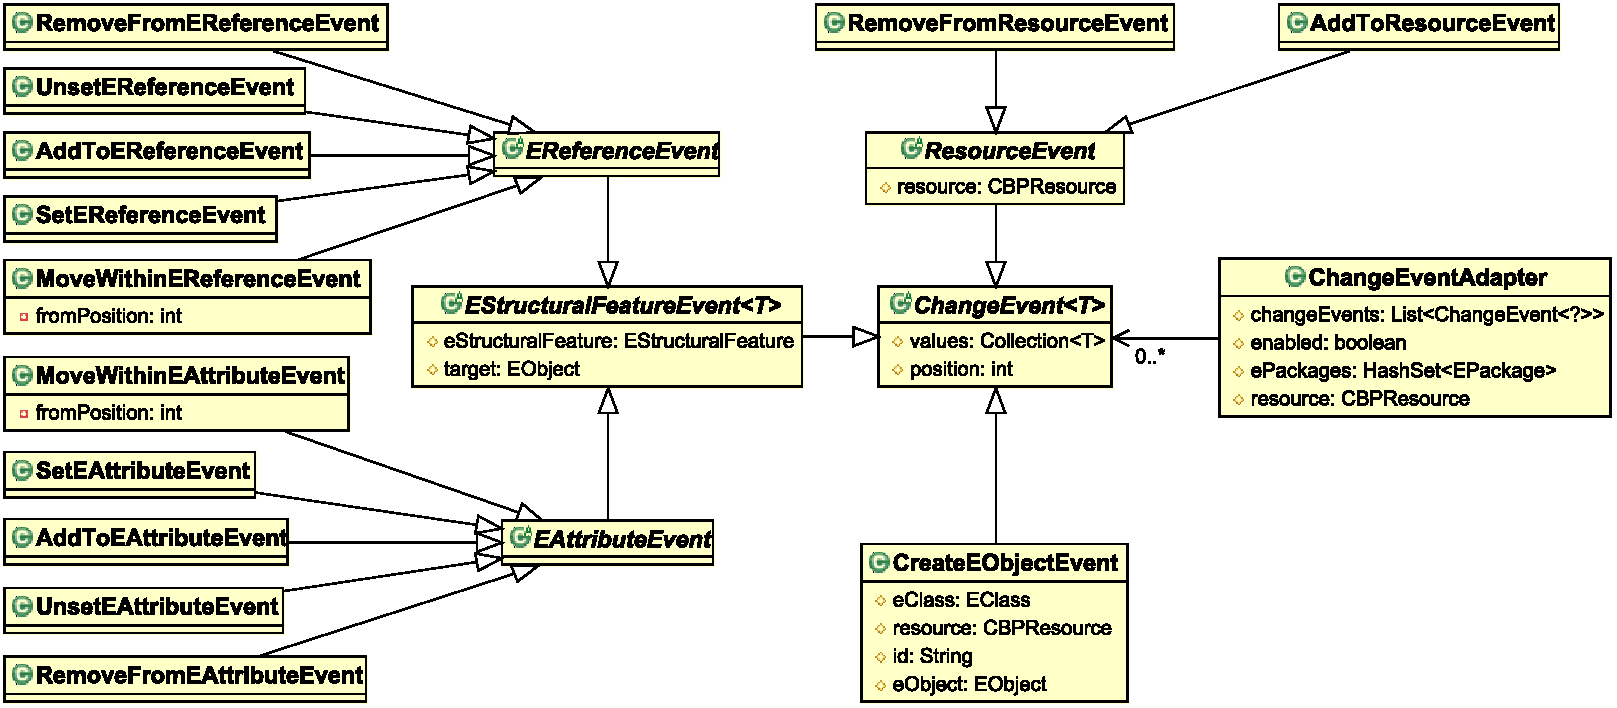
\includegraphics[width=\linewidth]{events}
\caption{Event classes to represent changes of models.}
\label{fig:events}
\end{figure*}

Since not all change events are relevant to change-based persistence (e.g. EMF also produces change notifications when listeners/adapted are added/removed from the model), we have defined a set of event classes to represent events of interest. The event classes are depicted in Figure \ref{fig:events} as subclasses of the \textsf{ChangeEvent} abstract class.

EMF has dedicated classes to express the graph structure of a model, such as \textsf{EStructuralFeature} can be \textsf{EReference} or \textsf{EAttribute}, it can have single value or multi values (e.g., Integer, String), the value(s) of \textsf{EStructuralFeature} can be type of \textsf{EObject} or primitive, the \textsf{EReference} can be type of containment or non-containment, and etc. These characteristics drive the design of the prototype to have different subclasses of \textsf{ChangeEvent} also decide which attributes and methods should be defined in the class. 

The \textsf{ChangeEvent} class has a multi-valued \textsf{values} attribute which can accommodate both single-valued (e.g. set/add) or multi-valued events (e.g. addAll/removeAll). \textsf{ChangeEvent} can also accommodate different types of values, such as \textsf{EObject}s for \textsf{EReferenceEvents}, and primitive values (e.g. Integer, String) for \textsf{EAttributeEvents}. The \textsf{ChangeEvent} class also has a position attribute to hold the  index of an \textsf{EObject} or a literal when they are added to a \textsf{Resource}, \textsf{EReference}, or \textsf{EAttribute} with multiple values. 

Every time an \textsf{EObject} is added to the model, a globally unique id is assigned to the \textsf{EObject}, and a \textsf{CreateEObjectEvent} and an \textsf{AddToResourceEvent} are recorded. When an EObject is deleted, or moved to a containment \textsf{EReference} elsewhere in the model, a \textsf{RemoveFromResourceEvent}
is recorded.

\begin{lstlisting}[style=java,caption={Simplified Java code to handle notification events.},label=lst:javacode]
public class ChangeEventAdapter extends EContentAdapter {
...
@override
public void notifyChanged(Notification n) {
  ...
  switch (n.getEventType()) {
  ... // other events
  case Notification.UNSET: {
    if (n.getNotifier() instanceof EObject) {
      EStructuralFeature feature = (EStructuralFeature) n.getFeature();
      if (feature instanceof EAttribute) {
        event = new UnsetEAttributeEvent();
      } else if (feature instanceof EReference) {
        event = new UnsetEReferenceEvent();
      }
    } break;
  } 
  ... // other events
\end{lstlisting}	

The \textsf{ChangeEventAdapter} receives EMF change notifications in its \textsf{notifyChanged()} method and filters and transforms them into appropriate change events. As an example of how notifications are filtered and transformed, Listing \ref{lst:javacode} shows how the prototype handles \textsf{Notification.UNSET} events based on the type of the changed feature i.e. an \textsf{UnsetEAttributeEvent} is instantiated if the feature of the notifier is an \textsf{EAttribute}, or an \textsf{UnsetEReferenceEvent}  is created if the notifier is an \textsf{EReference}. The transformed instances are then stored into a list of events in \textsf{ChangeEventAdapter} (\textsf{changeEvents}) for persistence. 

To integrate seamlessly with the EMF framework and to eventually support multiple concrete change-based serialisation formats (e.g. XML-formatted representation for readability and binary for performance/size), the prototype implemented a \textsf{CBPResource} abstract class that extends EMF's built-in \textsf{ResourceImpl} class. The role of the abstract class is to encapsulate all change recording functionality, while the role of its concrete subclasses is to implement serialisation and de-serialisation. 
To save a model, \textsf{CBPXMLResourceImpl} persists changes in a line-based format where every change is serialised as a single-line XML document. In this way, when a model changes, the prototype can append the new changes to the end of the model file without serialising the entire model again. 
To load a model, \textsf{CBPXMLResourceImpl} de-serialises every line in the document as a change event and then re-executes it to re-construct the model.
The prototype also includes a \textsf{CBPXMLResourceFactory} class that extends EMF's \textsf{ResourceFactoryImpl}, as the factory class for change-based models. Figure \ref{fig:resources} shows the relationships between these classes.

\begin{figure}[th]
\centering
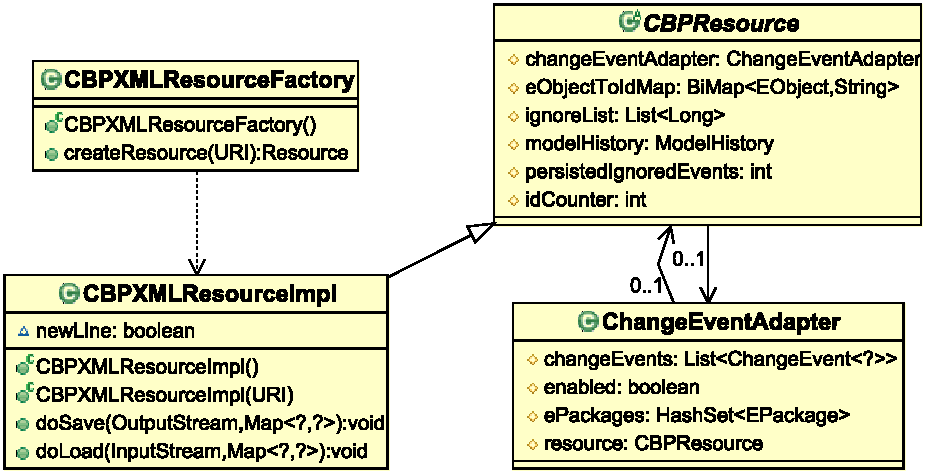
\includegraphics[width=\linewidth]{resources}
\caption{Factory, resources, and ChangeEventAdapter classes.}
\label{fig:resources}
\end{figure}

%Listing \ref{lst:javacode_resource} shows an example how to use the prototype in a Java code. Lines 1-8 demonstrate how to initialise and save a model using the prototype. First, the code creates an instance of \textsf{CBPResource}, \textsf{cbpResource}, using \textsf{CBPXMLResourceFactory} and specify its file as \textsf{helloworld.cbpxml} using \textsf{URI}. The code than executes method \textsf{startNewSession} of \textsf{cbpResource}. This method adds a change event to indicate the start of editing session as depicted at line 1 in Listings \ref{lst:cbp_origin} and \ref{lst:cbp_left}.
%The code then uses \textsf{UMLFactory} to create an element, \textsf{model}, of UML2's \textsf{Model}. The code adds element \textsf{model} into \textsf{cbpResource} and set the name to ``Hello World''. The code then saves the model in change-based format using method \textsf{save} and then unload \textsf{cbpResource}. Lines 9-12 demonstrate how to replay (load) the model that previously has been saved and then print the name of the first element in \textsf{cbpResource} which is expected to print ``Hello World'' text.
%
%\vspace{-20pt}
%\begin{lstlisting}[style=java,caption={An example how to use \textsf{CBPResource} in Java code.},label=lst:javacode_resource]
%/* initialise, save, and unload */
%CBPResource cbpResource = (CBPResource) (new CBPXMLResourceFactory()).createResource(URI.createFileURI("helloworld.cbpxml"));
%cbpResource.startNewSession("Initial");
%Model model = UMLFactory.eINSTANCE.createModel();
%cbpResource.getContents().add(model);
%model.setName("Hello World");
%cbpResource.save(null);
%cbpResource.unload();
%
%/* load and print */
%cbpResource.load(null);
%model = (Model) cbpResource.getContents().get(0);
%System.out.println(model.getName()); // expected output: "Hello World"
%\end{lstlisting}

\subsection{Benefits and Novel Capabilities}
\label{sec:benefits_and_novel_capabilities}

The proposed change-based model persistence also can deliver a wide range of benefits and novel capabilities, compared to the currently prevalent state-based representations, some of which are discussed below.

\begin{itemize}
\item With appropriate tool support, modellers will be able to ``replay'' (part of) the change history of a model (e.g. to understand design decisions made by other developers, for training purposes). This can be partly achieved in state-based approaches if models are stored in a version-control repository (e.g. Git). However, the granularity would only be at the commit level.
\item By analysing models serialised in the proposed representation, modelling language and tool vendors will develop more profound insights into how modellers use these languages/tools in practice and utilise this information to guide the evolution of the language/tool. An early prototype in this direction is discussed in \cite{polack2019towards}.
\item By attaching additional information to each session (e.g. the developer's id, references to external documents/URLs), sequences of changes can be traced back to the developer that made them or to requirements/bug reports that triggered them.
\item Persisting changes to large models after an editing session will be significantly faster than serialising the entire state of the model, as only changes made during the session will need to be appended to the model file.
\item The performance and precision of model comparison and merging can be substantially improved, particularly for large models with shared editing histories.
\end{itemize}

\subsection{Challenges}
\label{sec:challenges}

Change-based model persistence also comes with several challenges, such as loading overhead and fast-growing model files. 
\begin{itemize}
\item \emph{Loading overhead}. While, as discussed above, persisting changes to large models is expected to be much faster and resource-efficient compared to state-based approaches, loading models into memory by naively replaying the entire change history is expected to have a significant overhead. To address this challenge, we have developed two solutions that reduce the cost of change-based model loading. Firstly, we record and ignore events -- events that are later overridden or cancelled out by other events -- \cite{yohannis2018towards}. Secondly, we propose a hybrid model persistence format in which models are loaded from stated-based persistence, but changes are persisted into both change-based and state-based representation \cite{DBLP:conf/models/YohannisRPK18}. 
\item \emph{Fast-growing Model Files}. For the fast-growing model files challenge, persisting models in a change-based format means that model files will keep growing in size during their evolution significantly faster than their state-based counterparts. Future work is required to address this challenge.     
\end{itemize}



\section{Running Example (Continue)}
\label{sec:runnnig_example_continue}
Using the change-based model persistence presented in Section \ref{sec:emf_change_based_persistence}, instead of only persisting the models in Figure \ref{fig:class_diagram_rpg} in state-based format, we can also persist the complete history of changes of the models in change-based format. 

\begin{lstlisting}[style=eol,caption={Change-based representation of the original version in Figure \ref{fig:class_diagram_origin}.},label=lst:cbp_origin]
session "Jane-01"
create character type Class
set character.name from null to "Character" 
create attack type Operation
set attack.name from null to "attack" 
add attack to character.operations at 0
create gem type Parameter
set gem.name from null to "gem" 
add gem to attack.parameters at 0
create target type Parameter
set target.name from null to "target" 
add target to attack.parameters at 1
create weapon type Parameter
set weapon.name from null to "weapon" 
add weapon to attack.parameters at 2
create troll type Class
set troll.name from null to "Troll" 
create giant type class
set giant.name from null to "Giant"
create cast type Operation
set cast.name from null to "smash"
add cast to giant.operations at 0
create knight type Class
set knight.name from null to "Knight"
create smash type Operation
set smash.name from null to "smash"
add smash to knight.operations at 0
create mage type Class
set mage.name from null to "Mage" 
\end{lstlisting}

As an example, the complete history of changes made by Jane to construct the original version in Figure \ref{fig:class_diagram_origin} is also persisted in a change-based model representation as in Listing \ref{lst:cbp_origin}. The change events (Listing \ref{lst:cbp_left}) made by Bob is appended to Jane's original change events. Thus, the change events that represent Bob's version (Figure \ref{fig:class_diagram_left}) consists of the original change events and the change events (Listing \ref{lst:cbp_left}) made by him; only the appended changes are presented on the list. The change events that represents Alice's version (Figure \ref{fig:class_diagram_right}) is presented in Listing \ref{lst:cbp_right}. One clear advantage of change-based model persistence is that, from Listing \ref{lst:cbp_left}, we can immediately know all the changes made by Bob and Alice (starting from line 30) and identify all the elements that have been modified since Jane's version.  

\begin{lstlisting}[firstnumber=30,style=eol,escapechar=|,caption={The appended events made by Bob to produce the left version in Figure \ref{fig:class_diagram_left} (left version).},label=lst:cbp_left]
session "Bob-01"|\label{line:cbp_left_30}|
create leftGen type Generalization|\label{line:cbp_left_31}|
set leftGen.general to character|\label{line:cbp_left_32}|
set troll.generalization to leftGen|\label{line:cbp_left_33}|
set character.name from "Character" to "Hero"|\label{line:cbp_left_34}|
unset troll.generalization from leftGen to null composite l1|\label{line:cbp_left_35}|
set knight.generalization to leftGen composite l1|\label{line:cbp_left_36}|
move target in attack.parameters from 1 to 2|\label{line:cbp_left_37}|
unset cast.name from "cast" to null composite l2|\label{line:cbp_left_38}|
remove cast from giant.operations at 0 composite l2|\label{line:cbp_left_39}|
delete cast composite l2|\label{line:cbp_left_40}|
unset giant.name from "Giant" to null composite l2|\label{line:cbp_left_41}|
delete giant composite l2|\label{line:cbp_left_42}|
set troll.name from "Troll" to "Ogre"|\label{line:cbp_left_43}|
\end{lstlisting}

\begin{lstlisting}[firstnumber=30,style=eol,escapechar=|,caption={The appended events made by Alice to produce the right version in Figure \ref{fig:class_diagram_right} (right version).},label=lst:cbp_right]
session "Alice-01"|\label{line:cbp_right_30}|
move target in attack.parameters from 1 to 0|\label{line:cbp_right_31}|
remove smash from knight.operations at 0 composite r1|\label{line:cbp_right_32}|
add smash to giant.operations at 0 composite r1|\label{line:cbp_right_33}|
remove cast from giant.operations at 1 composite r2|\label{line:cbp_right_34}|
add cast to mage.operations at 0 composite r2|\label{line:cbp_right_35}|
create rightGen type Generalization|\label{line:cbp_right_36}|
set rightGen.general to character|\label{line:cbp_right_37}|
set troll.generalization to rightGen|\label{line:cbp_right_38}|
set character.name from "Character" to "Hero"|\label{line:cbp_right_39}|
unset troll.generalization from rightGen to null composite r3|\label{line:cbp_right_40}|
set mage.generalization to rightGen composite r3|\label{line:cbp_right_41}|
set troll.name from "Troll" to "Orc"|\label{line:cbp_right_42}|
\end{lstlisting}

Let's say the complete scenario that produces the models in Figures \ref{fig:class_diagram_origin}, \ref{fig:class_diagram_left}, and \ref{fig:class_diagram_right} as wells Listings \ref{lst:cbp_origin}, \ref{lst:cbp_left}, and \ref{lst:cbp_right} occured according to the following story.

Jane, as the technical leader, set up the initial model. The records of events during setting up the initial is recorded in the CBMP in List. \ref{lst:cbp_origin}. She created a class \textsf{Character} that contains an operation \textsf{attack} with three parameters: \textsf{gem}, \textsf{target}, and \textsf{weapon} (lines 2-15). She also created four other classes; \textsf{Troll} (lines 16-17), \textsf{Giant} (lines 18-22), \textsf{Knight} (lines 23-27), and \textsf{Mage} (lines 28-29). She then pushed her work to a change-based version control system. If her work is visualised in state-based format, the model looks like in Figure \ref{fig:class_diagram_origin}.

She then assigned this work to Bob and Alice. Both of them checked out this project to their own machine. Alice then started to continue the model. She then moved parameter \textsf{target} to the first place in operation \textsf{attack}'s parameters, because she thought it was more intuitive for programmers to think about the \textsf{target} first than the rest parameters (List. \ref{lst:cbp_right}, line 31). She also moved operation \textsf{smash} from class \textsf{Knight} to class \textsf{Giant} and operation \textsf{cast} from class \textsf{Giant} to class \textsf{Mage} as they are more reasonable to belong to their new classes (lines 32-35). Alice also created a generalisation relationship with id \textsf{rightGen} from class \textsf{Troll} to class \textsf{Character} (36-39). Bob also did the same thing except that his generalisation came with id \textsf{leftGen} (List. \ref{lst:cbp_left}, line 31-33). 

Later on, Jane then informed them that she wanted all good characters should be derived from a general, hero-like class, and the enemy should be the Orcs not Trolls. She also instructed that Bob should focus on developing class \textsf{Knight} and Alice on class \textsf{Mage}. In consequence, Alice then changed the name of class \textsf{Character} from ``Character'' to ``Hero'' (the id of class \textsf{Hero} is still \textsf{character}) (line 39). Again, Bob did the same thing. He also changed the name of class \textsf{Character} from ``Character'' to ``Hero'' (line 34). Instead of creating a new generalisation relationship, both of them preferred to move the generalisation relationships that they had created to their assigned classes. Alice moved generalisation \textsf{rightGen} from class \textsf{Troll} to class \textsf{Mage} (lines 40-41), and Bob move generalisation \textsf{leftGen} from class \textsf{Troll} to class \textsf{Knight} (lines 35-36). Bob also moved parameter \textsf{target} in operation \textsf{attack} to the last index as he thought setting target as the last parameter was intuitive (line 37), and deleted the class {Giant}, and unfortunately, he deleted class \text{Giant} accidentally (lines 38-42). The class diagrams of Bob and Alice's models are visualised in Figures \ref{fig:class_diagram_left} and \ref{fig:class_diagram_right} respectively. Lastly, Alice changed the \textsf{name} of class \textsf{Troll} to ``Orc'' (line 42) while Bob changed it to ``Ogre'' (line 43).  

In Listings \ref{lst:cbp_right} and \ref{lst:cbp_left}, we also introduce composite events -- lines with keyword \textsf{composite} -- that represent composite change events. 
Composite change events are events that should be treated as one composition -- identified with the same composite id. 
For example, moving an element from a container to another container is a composite event since it consists of two change events: 
removing/unsetting the element from its source container and adding/setting it to its target container (lines 40-41 in Listing \ref{lst:cbp_right}).



\section{Existing Conflict Detections in Models}
\label{sec:existing_conflict_detections}

In this section, we discuss two existing model conflict detection approaches. First, we describe the state-based conflict detection applied in EMF Compare \cite{emfcompare2018developer}, and, second, we explain the existing change-based conflict detection performed by EMF Store \cite{emfstore2019what,koegel2010operation}. Both are used as baselines in our against the change-based conflict detection method we propose in Section \ref{sec:emf_cbp_conflict_detection}.

\begin{table*}[ht]
\centering
\caption{Conflicting change events identified using EMF Compare based on the case in Figure \ref{fig:class_diagram_rpg}.}
\label{table:emfc_conflicts}
\begin{tabular}{|p{0.04\linewidth}|p{0.37\linewidth}|p{0.37\linewidth}|
		p{0.11\linewidth}|}
	\hline
	\textbf{ID} & 
	\textbf{Left Change Events (Bob)} & 
	\textbf{Right Change Events (Alice)} & 
	\textbf{Type}\\ 
	\hline
	EC1 & 
	set character.name from "Character" to "Hero" & 
	set character.name from "Character" to "Hero" & 
	pseudo \\
	\hline
	EC2 & set troll.name from "Troll" to "Ogre" & 
	set troll.name from "Troll" to "Orc & 
	real \\ 
	\hline
	EC3 & 
	delete cast
	& 
	\begin{minipage}[t]{\linewidth}
		\raggedright
		\begin{itemize}[leftmargin=0pt]
			\setlength
			\item[] remove cast from giant.operations at 0
			\item[] add cast to mage.operations at 0
		\end{itemize}
	\end{minipage}
	& 
	real, non-applicability\\
	\hline
	EC4 & 
	delete giant
	& 
	\begin{minipage}[t]{\linewidth}
		\raggedright
		\begin{itemize}[leftmargin=0pt]
			\setlength
			\item[] remove smash from knight.operations at 0
			\item[] add smash to giant.operations at 0
		\end{itemize}
	\end{minipage}
	& 
	real, non-applicability\\
	\hline
\end{tabular}
\end{table*}

\subsection{State-based Conflict Detection (EMF Compare)}
\label{sec:emfcompare_conflict_detection}

In this study, we select EMF Compare \cite{emfcompare2018developer} as an example tool to explain conflict detection in state-based model persistence. We also use it as a benchmark in the comparative evaluation of this paper. It is selected due to its maturity and ongoing development activity -- 4,682 commits and 103 releases on GitHub \cite{github2019emfcompare}. Another implementation of state-based conflict detection is EMF DiffMerge \cite{eclipse2019emfdiffmerge}. However, its comparison approach is similar to EMF Compare \cite{eclipse2019emfdiffmerge}, and it is less mature compared to EMF Compare -- only 442 commits and 20 releases on GitHub \cite{github2019emfdiffmerge}.

In state-based model comparison, a conflict occurs when the states of an element or a feature are different in two different versions of a model that are being compared. In other words, it can be said that the applied change events that cause the difference are in conflict since they produce two different states. Unfortunately, state-based persistence does not record change events that cause the differences. Thus, the change events have to be identified through model differencing \cite{emfcompare2018developer,yohannis2019efficient}. 

Let’s say that we have three versions of model $M$, the original shared version $m_{o}$ and two other modified versions: the left version $m_{l}$ and the right version $m_{r}$. There are also two lists of identified change events, left change events $C_{L}$ and right change events $C_{R}$. These lists are obtained by differencing $m_{l}$ to $m_{o}$ and $m_{r}$ to $m_{o}$ using an LCS (Longest Common Subsequence) algorithm \cite{emfcompare2018developer,DBLP:journals/algorithmica/Meyers86}, where $C_{L}$ = $(c_{l1}$, $c_{l2}$, ..., $c_{lm})$, $C_{R}$ = $(c_{r1}$, $c_{r2}$, ..., $c_{rn})$, $m$ is the number of left change events in $C_{L}$ or $m = |C_{L}|$, and $n$ is the number of change events in $C_{R}$ or $n = |C_{R}|$. Applying $C_{L}$ to model $m_{o}$ transforms it into model $m_{l}$, and applying $C_{R}$ to model $m_{o}$ transforms it into model $m_{r}$. These derived change events are be used to detect conflicts using Equations (\ref{eq:state_real_conflict}), (\ref{eq:state_pseudo_conflict}), and (\ref{eq:state_nonapplicability_conflict}).  

If state-based model differencing is used to derive left change events $C_{L}$ from the left and original versions (Bob's and Jane's versions) in Figure \ref{fig:class_diagram_rpg}, the following change events are obtained. 
\begin{lstlisting}[firstnumber=1,style=eol,caption={The derived, minimal change events to produce the left version (Bob's version) in Figure \ref{fig:class_diagram_left} from the original version (Jane's version).},label=lst:cbp_left_state]
move target in attack.parameters from 1 to 2
set character.name from "Character" to "Hero"
set troll.name from "Troll" to "Ogre"
create leftGen type Generalization composite l1
set leftGen.general from null to character composite l1
set knight.generalization from null to leftGen composite l1
unset cast.name from "cast" to null composite l2
remove cast from giant.operations at 0 composite l2
delete cast composite l2
unset giant.name from "Giant" to null composite l3
remove giant from resource at 2 composite l3
delete giant composite l3
\end{lstlisting}

And following list is the derived change events for $C_{R}$ that are obtained from the right and original versions (Alice's and Jane's versions) in Figure \ref{fig:class_diagram_rpg}. 
\begin{lstlisting}[firstnumber=1,style=eol,caption={The derived, minimal change events to produce the right version (Alice's version) in Figure \ref{fig:class_diagram_right} from the original version (Jane's version).},label=lst:cbp_right_state]
move gem in attack.parameters from 0 to 1
set character.name from "Character" to "Hero"
set troll.name from "Troll" to "Orc"
remove smash from knight.operations at 0 composite r1
add smash to giant.operations at 0 composite r1
create rightGen type Generalization composite r2
set rightGen.general to character composite r2
set mage.generalization to rightGen composite r2
remove cast from giant.operations at composite r3
add cast to mage.operations at 0 composite r3
\end{lstlisting}

Both Listings \ref{lst:cbp_left_state} and \ref{lst:cbp_right_state} are derived change events. They are a minimal sequence of change events that can produce $m_{l}$ and $m_{r}$ from $m_{o}$ respectively, but not necessarily the real changes made by Bob and Alice. For example, Bob and Alice may have created and then deleted a new class in the process or modified a feature but later decided to set it back to its initial value.

\textbf{Real Conflict}. In state-based model comparison, two change events, $c_{l}$ and $c_{r}$, are in conflict if both are applied to a same element $e_{o}$ but produce two different eventual states where $!$ is used as the operator for expressing that two change events are in conflict (\ref{eq:state_real_conflict}). EMF Compare \cite{emfcompare2018developer} classifies this conflict as a \textsf{REAL} conflict. For example, Bob changed the \textsf{name} of \textsf{troll} to ``Ogre'' (Listing \ref{lst:cbp_left_state}) while Alice modified it to ``Orc'' (Listing \ref{lst:cbp_right_state}). 
\begin{equation} \label{eq:state_real_conflict}
e_{o} + c_{l} \not\equiv e_{o} + c_{r} \Rightarrow c_{l}\;!\;c_{r}
\end{equation} 
\textbf{Non-applicability}. A \textsf{REAL} conflict also occurs when applying a change event $c_{l}$ to element $e_{o}$ makes $c_{r}$ inapplicable to element $e_{o}$. Therefore, change events $c_{l}$ and $c_{r}$ are in conflict (\ref{eq:state_nonapplicability_conflict}). 
For instance, Alice moved operation \textsf{smash} from class \textsf{Knight} to class \textsf{Giant} (Listing \ref{lst:cbp_right_state}) but this class was deleted by Bob (Listing \ref{lst:cbp_left_state}). Deleting class \textsf{Giant} makes the move inapplicable. 
\begin{equation} \label{eq:state_nonapplicability_conflict}
(e_{o} + c_{r} \not\equiv e_{o}) \wedge (e_{o} + c_{l} + c_{r} \equiv e_{o} + c_{l}) \Rightarrow c_{l}\;!\;c_{r}
\end{equation}
\textbf{Pseudo Conflict}. A conflict is classified as \textsf{PSEUDO} if the eventual states produced are equivalent. The \textsf{PSEUDO} means the conflict can be automatically resolved by choosing any of the conflicting changes since any of the changes produces the same eventual states (\ref{eq:state_pseudo_conflict}) \cite{emfcompare2018developer}. Symbol $!_{p}$ is used as the operator for expressing that two change events are in \textsf{PSEUDO} conflict. For example, both Bob and Alice changed the \textsf{name} of element \textsf{character} from ``Character'' to ``Hero'' (Listings \ref{lst:cbp_left_state} and \ref{lst:cbp_right_state}). 
\begin{equation} \label{eq:state_pseudo_conflict}
e_{o} + c_{l} \equiv e_{o} + c_{r} \Rightarrow c_{l}\;!_{p}\;c_{r}
\end{equation} 
Using Equations (\ref{eq:state_real_conflict}), (\ref{eq:state_nonapplicability_conflict}), and (\ref{eq:state_pseudo_conflict}) and information in Listings \ref{lst:cbp_left_state} and \ref{lst:cbp_right_state}, four conflicts can be identified -- presented in Table \ref{table:emfc_conflicts} along with their conflicting change events. Conflict \textsf{EC1} is a \textsf{pseudo} conflict since both modify the same class \textsf{character}'s feature \textsf{name} resulting the same end states, ``Hero'' or ``Hero''. Conflict \textsf{EC2} is a \textsf{REAL} conflict. Applying changing \textsf{troll}'s \textsf{name} to ``Ogre'' and \textsf{troll}'s \textsf{name} to ``Orc'' produces two different states -- ``Ogre'' and ``Orc''. Conflicts \textsf{EC3} and \textsf{EC4} are \textsf{REAL} non-applicability conflicts since if operation \textsf{cast} is deleted first then it cannot be moved -- removed and added -- from class \textsf{giant}'s \textsf{operations} to class \textsf{mage}'s \textsf{operations}, and if class \textsf{giant} is deleted first then operation \textsf{smash} cannot be moved -- removed and added -- from  class \textsf{knight}'s \textsf{operations} to class \textsf{giant}'s \textsf{operations}.

Conflict detection in state-based comparison might not be accurate since the derived differences/change events might not reflect the real historical changes of a model. For example, EMF Compare \cite{emfcompare2018developer} does not detect that Alice and Bob modified the same element -- parameter \textsf{target} -- as indicated by line 29 in List. \ref{lst:cbp_right} and line 35 in List. \ref{lst:cbp_left}. Using an LCS algorithm, the derived change events related to the feature \textsf{parameters} of element \textsf{attack}, which if presented as change events, are expressed as [\textsf{\small \textbf{move} target \textbf{in} attack.parameters \textbf{from} 1 \textbf{to} 2}] for Bob's version and [\textsf{\small \textbf{move} gem \textbf{in} attack.parameters \textbf{from} 1 \textbf{to} 2}] for Alice's version. Using (\ref{eq:state_real_conflict}), both change events are not in conflict since both change events modify two different elements, \textsf{target} and \textsf{gem}. The result is different if change-based approach is employed to detect conflicts using the change event records in Listings \ref{lst:cbp_left} and \ref{lst:cbp_right} which is explained in Section \ref{sec:emfstore_conflict_detection}.

\subsection{Change-based Conflict Detection (EMF Store)}
\label{sec:emfstore_conflict_detection}
EMF Store \cite{koegel2010emfstore} is an open-source tool that implements change-based model persistence for EMF models. It is a collaborative repository and versioning system that is specifically designed for models to answer existing versioning systems, such as Git and SVN, that focus heavily on text-based files \cite{emfstore2019what}. In addition, EMF Store follows the following rules to identify conflicts between change events \cite{koegel2010operation}. 

\textbf{Non-commutability}. In EMF Store, change events $c_{l}$ and $c_{r}$ are in conflict if applying them in different order to a same element $e_{o}$ produces two different eventual states \cite{koegel2010operation}. For example, Alice changed the \textsf{name} of class \textsf{Troll} to ``Orc'' (Listing \ref{lst:cbp_right}) while Bob renamed it to ``Ogre'' (Listing \ref{lst:cbp_left}). Applying Alice's change first to Bob's change results in the class' \textsf{name} equals to ``Ogre'', or ``Orc'' if the order is reversed.
\begin{equation} \label{eq:change_noncommutability}
e_{o} + c_{l} + c_{r} \not\equiv e_{o} + c_{r} + c_{l} \Rightarrow c_{l}\;!\;c_{r}
\end{equation} 
However, after examining the implementation \cite{eclipse2019emfstore}, even though two different change events produce equivalent eventual states, both change events are still treated in conflict by EMF Store (\ref{eq:ecbp_equal_end_states}). For example, both Bob and Alice changed the \textsf{name} of element \textsf{character} from ``Character'' to ``Hero'' (Listing \ref{lst:cbp_left} line \ref{line:cbp_left_34} and Listing \ref{lst:cbp_right} line \ref{line:cbp_right_39}). The reason is if we apply Bob's set event first, it changes \textsf{character}'s \textsf{name} from ``Character'' to ``Hero''. It is important to notice that after applying Bob's set event, the eventual value of \textsf{character}'s \textsf{name} is ``Hero''. Applying Alice's set event with previous value ``Character'' is inapplicable since it makes the sequence of the change events inconsistent; Bob's set event produces eventual value ``Hero'' which is not the previous value changed by Alice's set event, which is ``Character''. The same inconsistency still occurs even we apply these set events in different order.
\begin{equation} \label{eq:ecbp_equal_end_states}
\begin{split}
	e_{o} + c_{l} + c_{r} \equiv e_{o} + c_{l} + c_{r} \Rightarrow c_{l}\;!\;c_{r}
\end{split}
\end{equation} 
Moreover, a conflict occurs even when two different lists of change events, $C_{L}$ and $C_{R}$, produce eventual states that are equal to their initial states (\ref{eq:ecbp_equal_to_original_states}). For example, if both Bob and Alice alter \textsf{character}'s \textsf{name} from ``Character'' to ``Hero'' and then modify it back to ``Character'', both lists of change events are also treated in conflict.
\begin{equation} \label{eq:ecbp_equal_to_original_states}
\begin{split}
	e_{o} + C_{L} + C_{R} \equiv e_{o} + C_{R} + C_{L} \equiv e_{o}  \Rightarrow C_{L}\;!\;C_{R}
\end{split}
\end{equation} 
\textbf{Co-modification}. Thus, this leads to a new definition that a conflict occurs when two different change events modify a same element or feature regardless of the eventual states that they produce. 
\begin{equation} \label{eq:change_comodifiabilty}
(e_{o} + c_{l} \equiv e_{o} + c_{r}) \vee (e_{o} + c_{l} \not\equiv e_{o} + c_{r}) \Rightarrow c_{l}\;!\;c_{r}
\end{equation} 
\textbf{Non-applicability}. This non-applicability rule is the same with the non-applicability rule in the state-based conflict detection. Essentially, a conflict occurs when applying a change event $c_{l}$ to element $e_{o}$ makes $c_{r}$ inapplicable to element $e_{o}$. For instance, Alice moved operation \textsf{smash} from class \textsf{Knight} to class \textsf{Giant} (Listing \ref{lst:cbp_right}) but this class was deleted by Bob (Listing \ref{lst:cbp_left}). Deleting class \textsf{Giant} makes the move inapplicable. 
\begin{equation} \label{eq:change_nonapplicability}
(e_{o} + c_{r} \not\equiv e_{o}) \wedge (e_{o} + c_{l} + c_{r} \equiv e_{o} + c_{l}) \Rightarrow c_{l}\;!\;_{r}
\end{equation}
\textbf{Composite}. If change event $c_{l}$ is in conflict with change event $c_{r}$ where $c_{r}$ is a member of a composite change event $C_{cr}$ then change event $c_{l}$ is also in conflict with each change event $c_{n}$ in composite change event $C_{cr}$. For example, deleting class \textsf{Giant} is part of composite event \textsf{l2} (Listing \ref{lst:cbp_left}) and adding operation \textsf{smash} to class \textsf{Giant} is part of composite event \textsf{r1} (Listing \ref{lst:cbp_right}). Since they are in conflict according to (\ref{eq:change_nonapplicability}), all other change events in their composite events, \textsf{l2} and \textsf{r1}, also are in conflict.
\begin{equation} \label{eq:change_composite}
c_{l}\;!\;c_{r} \wedge c_{r} \in C_{cr} \Rightarrow c_{l} \;!\; c_{rn} \; | \; c_{rn} \in C_{cr}
\end{equation}

\begin{table*}[ht]
\centering
\caption{Conflicting change events identified using EMF Store in Listings \ref{lst:cbp_right} and \ref{lst:cbp_left}.}
\label{table:conflicts_emfs}
\begin{tabular}{|p{0.04\linewidth}|p{0.37\linewidth}|p{0.37\linewidth}|
		p{0.11\linewidth}|}
	\hline
	\textbf{ID} & 
	\textbf{Left Change Events (Bob)} & 
	\textbf{Right Change Events (Alice)} & 
	\textbf{Type}\\ 
	\hline
	ES1 & 
	\begin{minipage}[t]{\linewidth}
		\raggedright
		\begin{itemize}[leftmargin=0pt]
			\setlength
			\item[] set troll.generalization from null to left
			Gen
			\item[] unset troll.generalization from leftGen
			to null
			\item[] set knight.generalization from null
			to leftGen
		\end{itemize}
	\end{minipage} & 
	\begin{minipage}[t]{\linewidth}
		\raggedright
		\begin{itemize}[leftmargin=0pt]
			\setlength
			\item[] set troll.generalization from null to
			rightGen
			\item[] unset troll.generalization from rightGen
			to null
			\item[] set mage.generalization from null to
			rightGen
		\end{itemize}
	\end{minipage} & 
	co-modification,
	composite \\
	\hline
	ES2 & set character.name from "Character"
	to"Hero" & 
	set character.name from "Character"
	to "Hero" & 
	co-modification \\ 
	\hline
	ES3 & 
	move target in attack.parameters from
	1 to 2
	& 
	move target in attack.parameters from
	1 to 0
	& 
	non-applicability\\
	\hline
	ES4 & 
	\begin{minipage}[t]{\linewidth}
		\raggedright
		\begin{itemize}[leftmargin=0pt]
			\setlength
			\item[] unset cast.name from "cast" to null
			\item[] remove cast from giant.operations at 0
			\item[] delete cast type Operation
			\item[] unset giant.name from "Giant" to null
			\item[] delete giant
		\end{itemize}
	\end{minipage}
	& 
	\begin{minipage}[t]{\linewidth}
		\raggedright
		\begin{itemize}[leftmargin=0pt]
			\setlength
			\item[] remove cast from giant.operations at 0
			\item[] add cast to mage.operations at 0
			\item[] remove smash from knight.operations at 0
			\item[] add smash to giant.operations at 1
		\end{itemize}
	\end{minipage}
	& 
	non-applicability, composite\\
	\hline
	ES5 & 
	set troll.name from "Troll" to "Ogre" & 
	set troll.name from "Troll" to "Orc" & 
	co-modification\\ 
	\hline
\end{tabular}
\end{table*}

In change-based conflict detection, all change events applied to a model are readily available. Thus, the change events do not need to be derived through a diffing process. The availability of real historical changes can improve the accuracy of change detection since elements that have been changed can be identified according to fact -- not derivation. In consequence, it can detect conflicts that cannot be detected by state-based conflict detection. For example, in Listing \ref{lst:cbp_right} line 31, parameter \textsf{target} has been moved from index 1 to 0, while in Listing \ref{lst:cbp_left} line 37, it was moved from index 1 to 2. Since both change events modified the same parameter \textsf{target}, both change events can be identified in conflict using (\ref{eq:change_comodifiabilty}); the same parameter \textsf{target} is modified by two different change events. 

The drawback of EMF Store is that it treats two change events that modify the same element as they are in conflict regardless of the end states that they produce to the element \cite{DBLP:conf/sfm/BroschKLSWW12}. In common sense, two changes should not be in conflict if they are applied to the same element or feature and produce the same eventual states. Moreover, EMF Store does not have a classification that separates conflicts into \textsf{REAL} or \textsf{PSEUDO} conflicts, such as in EMF Compare, to automate conflict resolution. 

%For example, two change events in Listing \ref{lst:cbp_right} at line \ref{line:cbp_right_39} and Listing \ref{lst:cbp_left} at line \ref{line:cbp_left_35}, that change the same feature \textsf{name} from ``Character'' to the same value ``Hero'', are treated in conflict (Table \ref{table:conflicts_emfs} id ES2) using (\ref{eq:change_comodifiabilty}). EMF Compare classifies this kind of conflict as \textsf{PSEUDO} conflict which can be automatically resolved in merging only by selecting one of the conflicting change events and ignoring the other one.

Excluding eventual states in detecting conflicts also causes all change events related to \textsf{troll}'s \textsf{generalization} to be in conflict; all the feature's left-side events are in conflict with all its right-side events (Table \ref{table:conflicts_emfs}, ES1). Using the co-modification  (\ref{eq:change_comodifiabilty}) rule, we can detect that the setting and unsetting of \textsf{troll}' \textsf{generalization} to \textsf{leftGen} and \textsf{null} (Listing \ref{lst:cbp_left} lines \ref{line:cbp_left_33}, \ref{line:cbp_left_35}) are in conflict with the setting and unsetting of \textsf{troll}' \textsf{generalization} to \textsf{rightGen} and \textsf{null} (Listing \ref{lst:cbp_right} lines \ref{line:cbp_right_38}, \ref{line:cbp_right_40}). Moreoever, using composite (\ref{eq:change_composite}) rule, we can also identify that the setting of \textsf{knight}' \textsf{generalization} to \textsf{leftGen} (Listing \ref{lst:cbp_left} line \ref{line:cbp_left_36}) and the setting of \textsf{mage}' \textsf{generalization} to \textsf{rightGen} (Listing \ref{lst:cbp_right} line \ref{line:cbp_right_41}) are also part of the conflict ES1 since both events are in the same composite move events, \textsf{l1} and \textsf{r3}, with the unsetting of \textsf{troll}' \textsf{generalization} to  \textsf{null} (Listing \ref{lst:cbp_left} line \ref{line:cbp_left_35}, Listing \ref{lst:cbp_right} line \ref{line:cbp_right_38}).

In state-based conflict detection, case ES1 is not a conflict since the values of class \textsf{troll}'s feature \textsf{generalization} in the Jane's, Bob's, and Alice's versions are indentical -- all are null. Thus, there are no different \textit{derived} change events that modify class \textsf{troll}'s feature \textsf{generalization} in parallel. 

Conflict ES4 is a non-applicability, composite conflict. Moving element \textsf{smash} from class \textsf{knight} to class \textsf{giant} and moving element \textsf{cast} from class \textsf{giant} to class \textsf{mage} require the deletion of class \textsf{giant} to be executed later in order to be applicable. Conflict ES5 is can be detected with the co-modification  (\ref{eq:change_comodifiabilty}) rule. The states of \textsf{troll}'s \text{name} have been simultaneously modified to ``Ogre'' or ``Orc''.

\begin{table*}[]
\centering
\caption{The advantages and drawbacks of EMF Compare and EMF Store in detecting conflicts.}
\label{tab:accuracy_emfcompare_emfstore}
\begin{tabular}{|p{0.1\linewidth}|p{0.4\linewidth}|p{0.4\linewidth}|}
	\hline
	\textbf{Dimension}
	& \textbf{State-based Conflict Detection (EMF Compare)}
	& \textbf{Change-based Conflict Detection (EMF Store)}\\
	\hline
	\multicolumn{1}{|c|}{Advantages}
	&
	\begin{minipage}[t]{\linewidth}
		\raggedright
		\begin{itemize}[leftmargin=9pt]
			\setlength\itemsep{2pt}
			\item[-] detect \textsf{PSEUDO} conflict which can be automatically resolved when merging
			\item[-] conflicts detected are optimal since changes are derived thus avoid oversensitive conflict detection
			\item[]
		\end{itemize}
	\end{minipage}
	&
	\begin{minipage}[t]{\linewidth}
		\raggedright
		\begin{itemize}[leftmargin=9pt]
			\setlength\itemsep{2pt}
			\item[-] more accurate in detecting conflicts since changes are real history
			\item[-] in large models with moderate changes, it should perform faster than the state-based approach -- no need to derive changes since they are already available 
			\item[]
		\end{itemize} 
	\end{minipage}
	\\ 
	\hline
	\multicolumn{1}{|c|}{Drawbacks}
	&
	\begin{minipage}[t]{\linewidth}
		\raggedright
		\begin{itemize}[leftmargin=9pt]
			\setlength\itemsep{2pt}
			\item[-] less accurate in detecting conflicts since changes are derived -- not real changes
			\item[-] in large models, its performance should be slower the change-based approach since it performs 3-way comparison which requires 2-times model differencing to derive changes
			\item[-] in small models, it should perform faster than change-based approach
			\item[]
		\end{itemize}
	\end{minipage}
	&
	\begin{minipage}[t]{\linewidth}
		\raggedright
		\begin{itemize}[leftmargin=9pt]
			\setlength\itemsep{2pt}
			\item[-] treat all conflicts as \textsf{REAL} conflicts which demand user intervention for resolution
			\item[-] can be oversensitive in detecting conflicts since eventual states are not considered
			\item[-] in small models with excessive changes, it should perform slower than the state-based approach due to processing lots of change records
			\item[]
		\end{itemize} 
	\end{minipage}
	\\
	\hline                         
\end{tabular}
\end{table*}

\subsection{Summary}
\label{sec:summary}
The summary of the advantages and drawbacks between EMF Compare and EMF Store in detecting conflicts are presented in Table \ref{tab:accuracy_emfcompare_emfstore}. The state-based approach, represented by EMF Compare \cite{emfcompare2018developer}, does come with drawbacks. First, it cannot detect conflicts as accurately as change-based approaches can as their changes are derived rather than actual historical changes. Second, EMF Compare uses 3-way model comparison \cite{emfcompare2018developer} thus hypothetically, its conflict detection should perform relatively slower than the change-based approach, since it has to perform state-based model differencing twice to derive changes events: changes events between left and original versions, and change events between right and original versions. 

Change-based model conflict detection \cite{koegel2010operation}, represented by EMF Store \cite{emfstore2019what}, also has drawbacks. EMF Store purely works on comparing change events and detects conflicts based on predefined rules; it does not consider the eventual states of two versions that are being compared. Thus, two change events that modify the same feature are considered in conflict even though both change events produce the same eventual states. This condition can lead EMF Store to oversensitive conflict detection. 

\section{EMF CBP Conflict Detection}
\label{sec:emf_cbp_conflict_detection}
This section proposes a change-based model conflict detection that also considers the eventual states of modified elements. Thus, the performance and accuracy of model conflict detection can be improved -- compared to state-based conflict detection -- without being oversensitive -- as opposed to the change-based conflict detection of EMF Store.

The change-based model conflict detection proposed in this paper consists of three phases: event loading, partial element tree construction, and conflict computation. Conflict detection is not performed over all the elements of the model as opposed to state-based model differencing; instead, the approach only needs to compare the last sets of change events of the two models being compared, starting from the first line of both models are different. A simplified class diagram of the approach \cite{epsilonlabs2019emfcbp} is depicted in Figure \ref{fig:approach_class_diagram}. The three phases are described in detail below.

\begin{figure*}
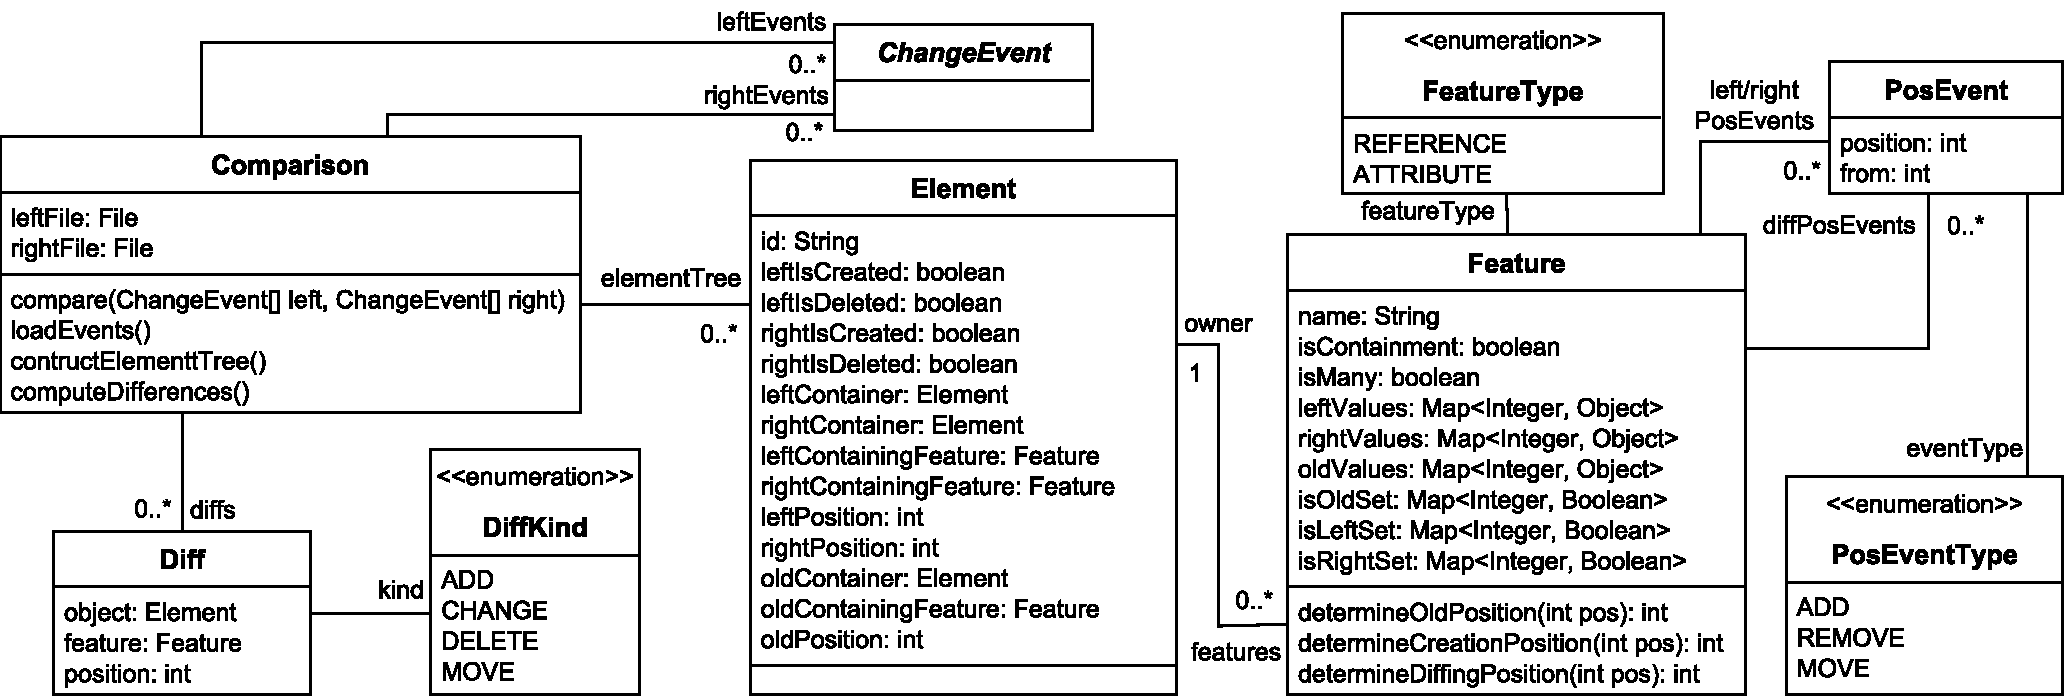
\includegraphics[width=\linewidth]{TreeClassDiagram}
\caption{A class diagram showing the core components of the change-based approach to speed up model differencing and conflict detection.}
\label{fig:approach_class_diagram}
\end{figure*}

The model conflict detection method proposed in this study basically performs similar steps to the procedure of change-based model differencing in our previous work \cite{yohannis2019efficient} but with some modification. The change-based model differencing itself consists of three phases: event loading, element tree construction, and diff computation. First, conflict detection still performs the event loading and element tree construction phases, but the diff computation phase is replaced with conflict computation phase. Second, during element tree construction, the conflict detection maps change events to the elements, features, and values that the change events modify. 

\subsection{Event Loading}
\label{sec:event_loading}
In the event loading phase, the implementation loads change events recorded in two change-based model persistence files into memory.
The most important aspect of this phase is the partial loading, as only lines starting from the position where the two files are different are loaded.
Thus, not the whole model needs to be traversed and loaded.
In this case, lines 1-29 in Listing \ref{lst:cbp_origin} are skipped. Only lines starting from line 30 in Listings \ref{lst:cbp_left} and \ref{lst:cbp_right} are loaded, yielding two partial -- left and right -- change-event models. 

\subsection{Element Tree}
\label{sec:tree_construction}
An element tree is a representation of the changes of model elements in the source and reference models. It contains detailed information about elements and their properties. It contains similar information to that captured in change lists in state-based model persistence and provides more information about the changes. For example, the element tree can keep track of a feature's old value and element/value's indexes inside multi-valued properties. The element tree only contains the partial states of affected elements of the original, left, and right models as depicted in Figures \ref{fig:left_element_tree_diagram} and \ref{fig:right_element_tree_diagram}.

To better understand the construction of an element tree from change events, we use the following running example using both change events in the Listings \ref{lst:cbp_left} and \ref{lst:cbp_right}. We start from the left change events. 

\subsubsection{Left Side}\label{sec:left_side}
In the first change event in Listing \ref{lst:cbp_left} at line \ref{line:cbp_left_30}, the change event is a \textsf{session} event. It marks that all the following change events until the final line or next \textsf{session} event are persisted in one batch when saving. At line \ref{line:cbp_left_31}, we can identify that Bob created a \textsf{Generalization} with id \textsf{leftGen}. Thus, in \textsf{elementTree}, an element with id \textsf{leftGen} is also created. To mark that an element is newly created in the session, we put a `+' sign at the left lower box of element \textsf{leftGen} in Figure \ref{fig:left_element_tree_diagram}.

\begin{figure*}[ht]
\centering
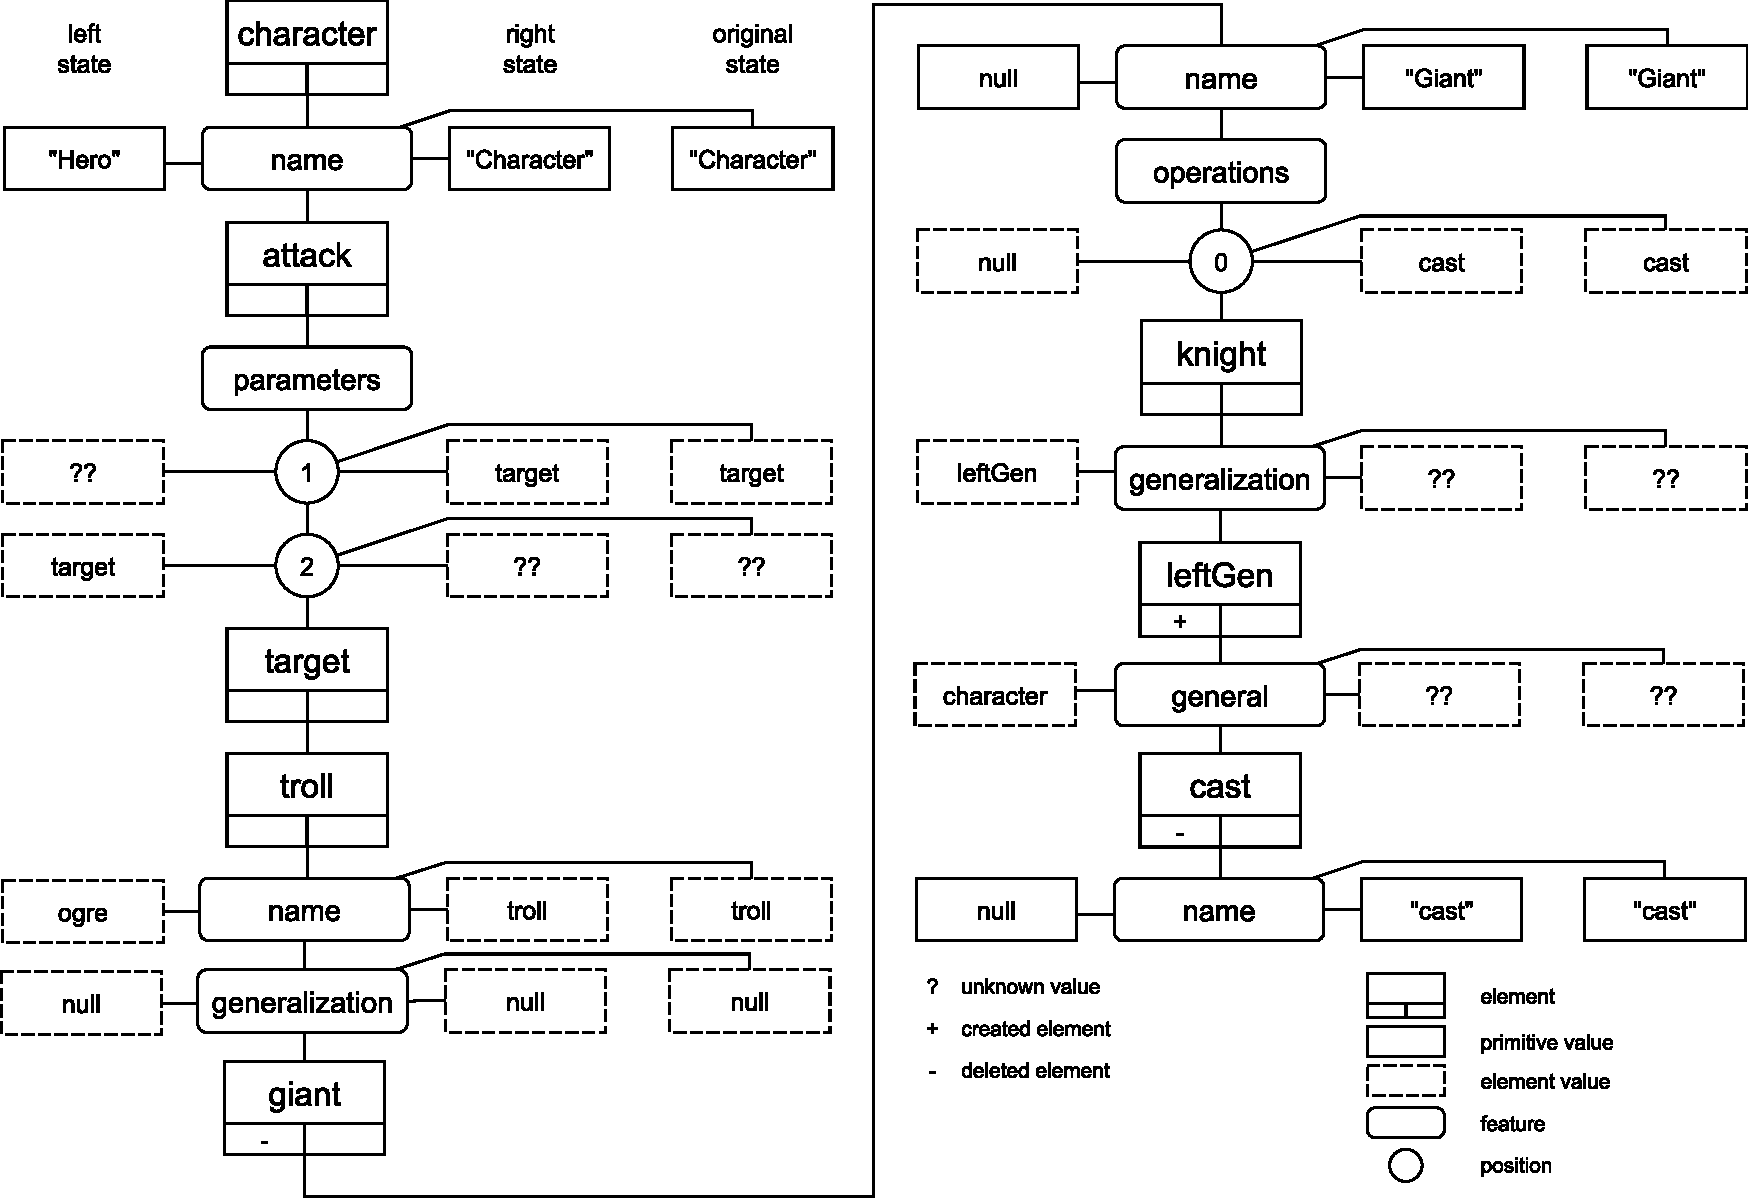
\includegraphics[width=\linewidth]{element_tree_game_left}
\caption{An element tree constructed using information contained in CBPs in Listing \ref{lst:cbp_left} (all left change events only).}
\label{fig:left_element_tree_diagram}
\end{figure*} 

At line \ref{line:cbp_left_32}, the feature \textsf{general} of \textsf{leftGen} is set to \textsf{character}. From the change event, we can recognise that \textsf{character} has existed since the previous version since it has not been created in the current editing session. Thus, we create an element with id \textsf{character} as well as the feature \textsf{general} of \textsf{leftGen} and put them in \textsf{elementTree} and then set the value of \textsf{general} to \textsf{character} on the left side. We also do the same routine to \textsf{troll} and \textsf{generalization} at line \ref{line:cbp_left_33}, adding element \textsf{troll} and feature \textsf{generalization} to \textsf{elementTree} and set the value of feature \textsf{generalization} to \textsf{leftGen} on the left side of the \textsf{elementTree}. 

Change event at line \ref{line:cbp_left_34}, changes \textsf{character}'s \textsf{name} from ``Character'' to ``Hero''. From the change event, we can identify that \textsf{character} has existed before. Thus, we create element \textsf{character} and feature \textsf{name} into \textsf{elementTree}. We also set the value of \textsf{name} to ``Hero'' on the left side. Since this set change event is the first event for \textsf{character}'s \textsf{name}, we can infer that original value of \textsf{name} is ``Character''. Thus, we set \textsf{name}'s value to ``Character'' on the original side. The value of \textsf{name} on the right side is also set to ``Character'' but will be modified later once we process the right change events (Alice's change events) if there is any change event that affects it. The same routine is also applied when we process the change event at line \ref{line:cbp_left_43} later.

Lines \ref{line:cbp_left_35} and \ref{line:cbp_left_36} are the changes events of  composite move event \textsf{l1}. Element \textsf{leftGen} is removed (unset) from \textsf{troll}'s \textsf{generalization} and then is assigned (set) to \textsf{knight}'s \textsf{generalization}. From these change events, we can identify that element \textsf{knight} also already existed since the original version. Thus, we add it into \textsf{elementTree} together with its  \textsf{generalization} feature. Element \textsf{troll} and its  \textsf{generalization} feature are not added into \textsf{elementTree} any more since they were already added when processing line \ref{line:cbp_left_33}. In \textsf{elementTree}, we set \textsf{troll}'s \textsf{generalization} to null since element \textsf{leftGen} is moved to \textsf{knight}'s \textsf{generalization}.

At line \ref{line:cbp_left_37}, \textsf{target} is moved from index 1 to 2 in \textsf{attack}'s \textsf{parameters}. From the change event, we can identify that there has been element \textsf{target} contained in \textsf{attack}'s \textsf{parameters} at index 1 since the original version. Thus, we put element \textsf{target} and element \textsf{attack} and its \textsf{parameters} feature into \textsf{elementTree}. We also create a map on the left side with a key `2' and a value that points to element \textsf{target} for feature \textsf{parameters}, indicating \textsf{target} is at index 2 in the left version. Since it is the first change event that moves \textsf{target}, we can decide that \textsf{target} is at index 1 in the original version. Thus, we create another map on the original side a map on the left side with a key `1' and a value that also points to \textsf{target}. We also perform this routine to the right side of feature \textsf{parameters}, creating a map with a key `1' and a value that also points to \textsf{target}. It will be modified later once we process the right change events (Alice's change events) if there is any change event that affects the index of \textsf{target}.

Lines \ref{line:cbp_left_38} to \ref{line:cbp_left_42} are the change events of  composite delete event \textsf{l2}; a deletion of element \textsf{giant}. 
Deletion of an element unsets all the features of the elements and their sub-elements, removes the sub-elements from their containers, and deletes the sub-elements and the element from the model. 
As can be noticed,  at line \ref{line:cbp_left_38}, the value of \textsf{cast}'s \textsf{name}  is unset from ``cast'' to null. From the change event, we know that cast has been existed since the original version. Thus, we add element \textsf{cast} and its feature \textsf{name} to \textsf{elementTree} and set its value null on the left side and ``cast'' on the origin and right sides. 

At line \ref{line:cbp_left_39}, \textsf{cast} is removed from \textsf{giant}'s \textsf{operations} at index 0. From it, we can identify that \textsf{giant} and its feature \textsf{operations} exists, and \textsf{cast} is contained in \textsf{giant}'s \textsf{operations} at index 0 in the original version. Thus, we create element \textsf{giant} and its feature \textsf{operations} in \textsf{elementTree}. Three maps also are created in \textsf{operations} for the three sides. Each map contains a key `0', indicating index, and a value that points to element \textsf{cast} except on the left side the value is null since \textsf{cast} is removed from \textsf{giant}'s \textsf{operations}. The deletion of \textsf{cast} at line \ref{line:cbp_left_40} marks \textsf{cast} in \textsf{elementTree} with `-' sign on the left side indicating that the element is deleted from the model in the left version.

Change event at line \ref{line:cbp_left_41} is similar to change event at line At line \ref{line:cbp_left_38} except that it is applied to \textsf{giant}'s \textsf{name}. Since \textsf{giant} has existed in \textsf{elementTree}, only the feature \textsf{name} is added. Its value is set to null on the left side and ``Giant'' on the origin and right sides. The deletion of \textsf{giant} at line \ref{line:cbp_left_42} marks \textsf{giant} in \textsf{elementTree} with `-' sign indicating that the element is deleted from the model in the left version.

Figure \ref{fig:left_element_tree_diagram} illustrates the state of the \textsf{elementTree} after all left change events have been processed. As can be seen, the \textsf{elementTree} exhibits the partial states of the original, left, and right models at once. 

\subsubsection{Right Side}\label{sec:right_side}
In Listing \ref{lst:cbp_right}, similar to processing the left change events, the processing of the right change events (Alice's version) starts with processing the session event at line \ref{line:cbp_right_30}. At line \ref{line:cbp_right_31}, \textsf{target} is moved from index 1 to 0 in \textsf{attack}'s \textsf{parameters}. Since the index of \textsf{target} is already determined when processing the change event, we only determine the index of \textsf{target} on the right side. We unset the value of key `1' on the right side to null and create a new key `0' that maps its value to \textsf{target}.

Composite move event \textsf{r1} at lines \ref{line:cbp_right_32} and \ref{line:cbp_right_33} moves \textsf{smash} from \textsf{knight}'s \textsf{operations} to \textsf{giant}'s \textsf{operations}. From this move event, we can identify \textsf{smash} is no longer in \textsf{knight}'s \textsf{operations} but contained in \textsf{giant}'s \textsf{operations} on the right side. Element \textsf{smash} has never existed in \textsf{elementTree}. So, we create and add \textsf{smash} to \textsf{knight}'s \textsf{operations} at index 0 on the origin side and to \textsf{giant}'s \textsf{operations} at index 0 on the right side. Since \textsf{smash} is not modified on the left side and no other change events applied to \textsf{knight}'s \textsf{operations}, we can determine that \textsf{smash} is at index 0 in \textsf{giant}'s \textsf{operations} on the left side.

Lines \ref{line:cbp_right_34} and \ref{line:cbp_right_35} are change events that constitute composite move event \textsf{r2}.  It  moves \textsf{cast} from \textsf{giant}'s \textsf{operations} to \textsf{mage}'s \textsf{operations}. From this move event, we can identify \textsf{cast} is no longer in  \textsf{giant}'s \textsf{operations} but now exists in \textsf{mage}'s \textsf{operations} on the right side. Element \textsf{mage} and its feature \textsf{operations} have never existed in \textsf{elementTree}. So, we create and add them to \textsf{elementTree} and add \textsf{cast} to \textsf{mage}'s \textsf{operations} on the right side.

At line \ref{line:cbp_right_36}, we can identify that Alice created a \textsf{Generalization} with id \textsf{rightGen}. Thus, in \textsf{elementTree}, an element with id \textsf{rightGen} is also created. Since it has just been created in the active session, the element is marked with '+' sign in \textsf{elementTree} on the right side. At line \ref{line:cbp_right_37}, we can also identify that feature \textsf{general} should be added to \textsf{rightGen} in \textsf{elementTree} and the value is set to \textsf{character} on the right side. We also set \textsf{mage}'s \textsf{operations} to \textsf{rightGen} on the right side of  \textsf{elementTree} according to the change event at line \ref{line:cbp_right_38}. 

\begin{figure*}[]
\centering
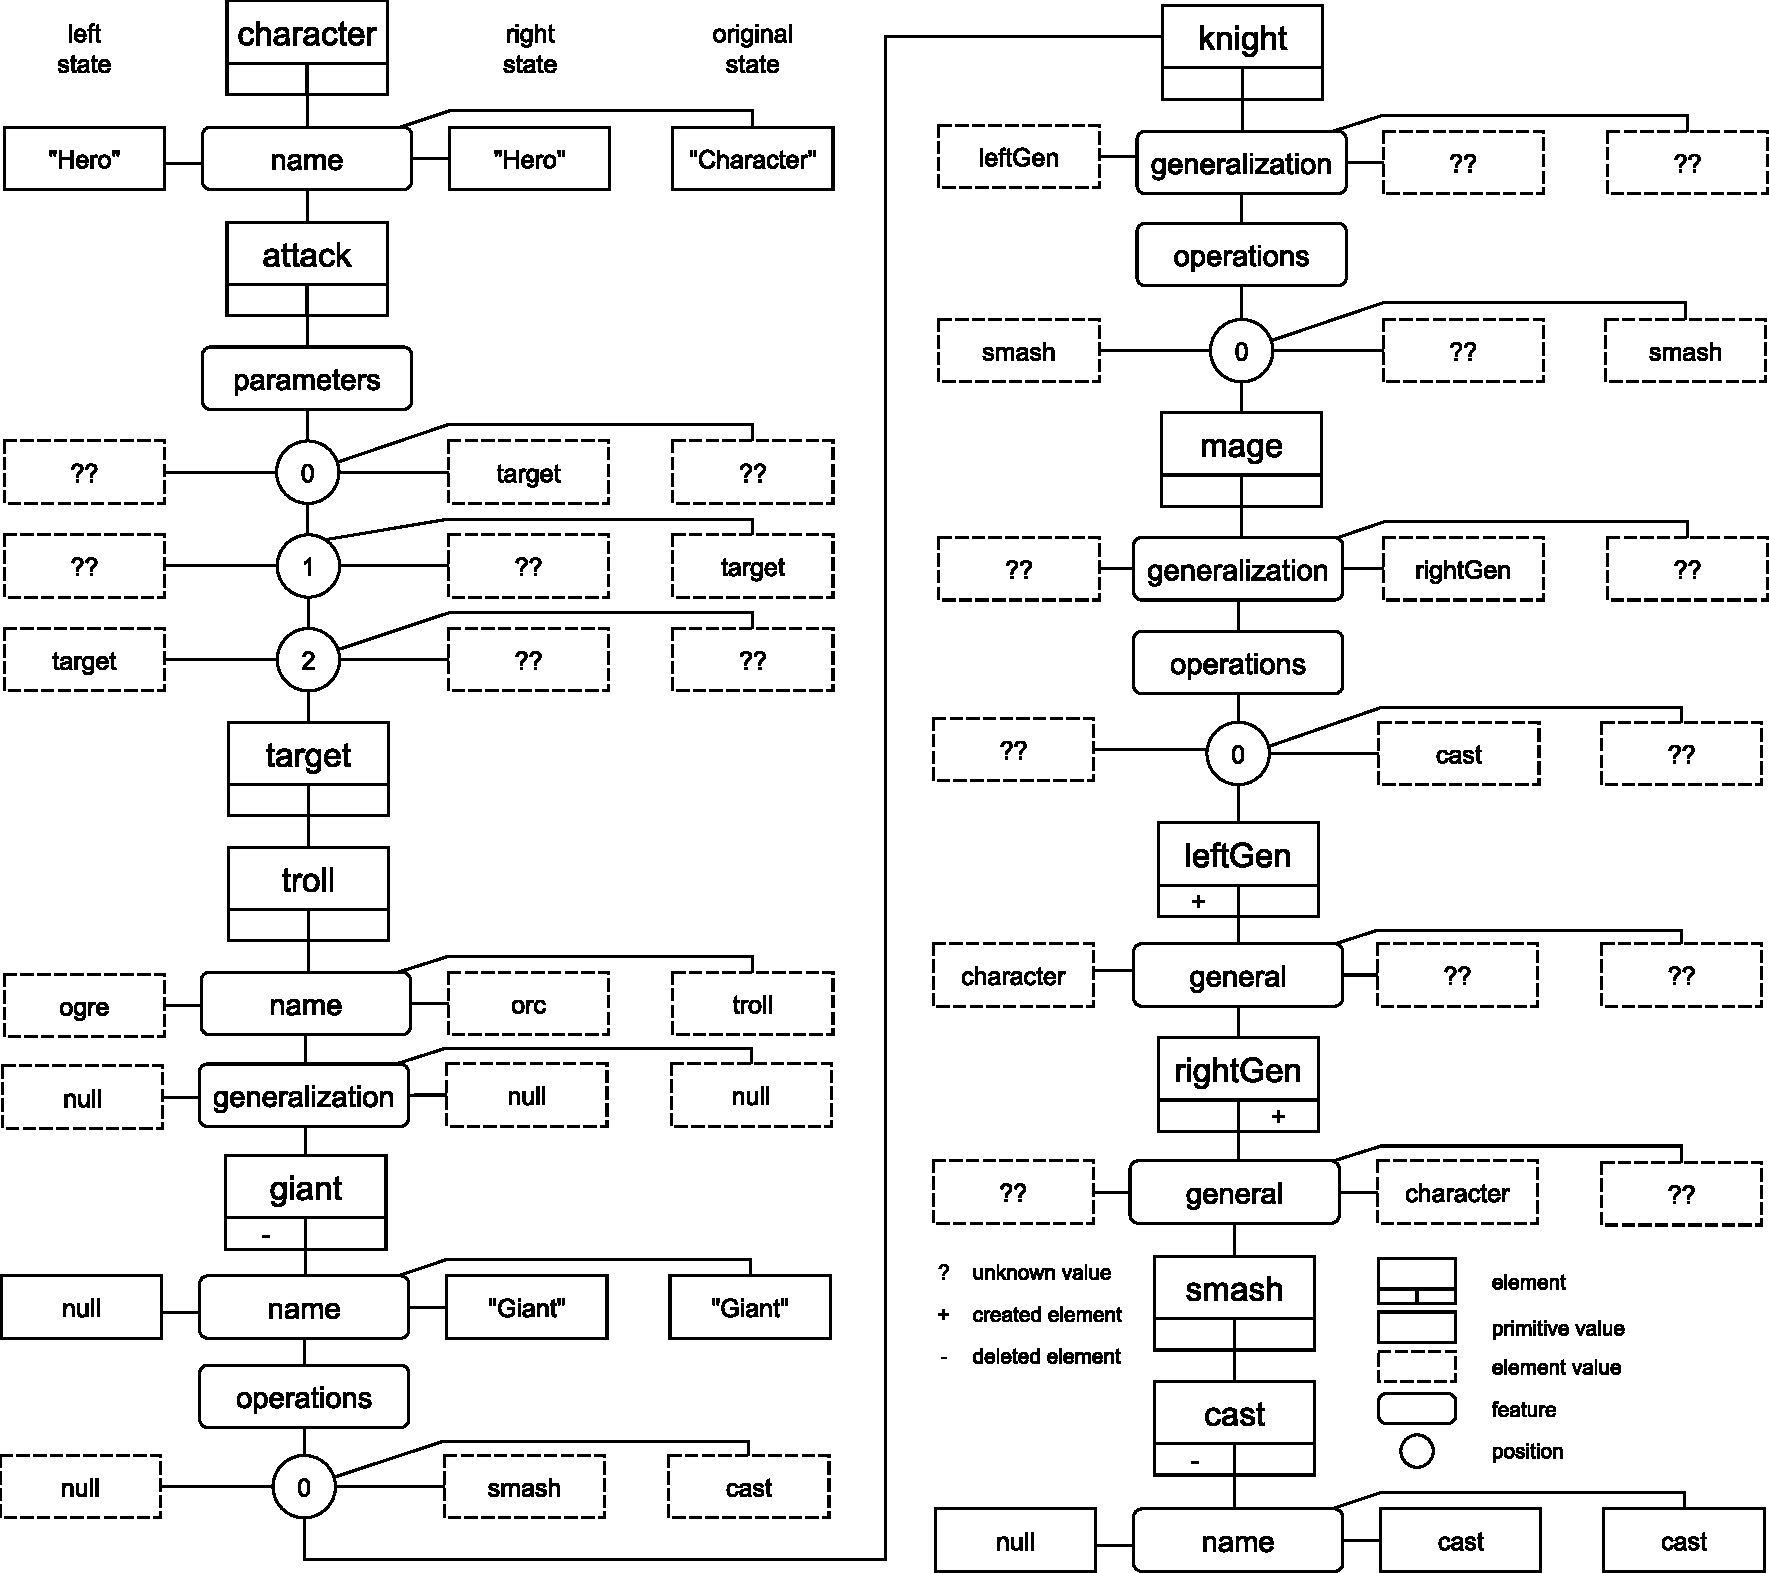
\includegraphics[width=\linewidth]{element_tree_game_right}
\caption{An element tree constructed using information contained in CBPs in Listings \ref{lst:cbp_left} and \ref{lst:cbp_right} (all left and right change events).}
\label{fig:right_element_tree_diagram}
\end{figure*} 

Change event at line \ref{line:cbp_right_39}, change \textsf{character}'s \textsf{name} from ``Character'' to ``Hero''. Since \textsf{character} and its feature \textsf{name} already exist in \textsf{elementTree}, we only set \textsf{name}'s value to ``Hero'' on the right side; the original value has already been assigned when processing left change events. We apply the same routine when processing the change event at line \ref{line:cbp_right_42} later.

Composite move event \textsf{r3} at lines \ref{line:cbp_right_40} and \ref{line:cbp_right_41} moves \textsf{rightGen} from \textsf{troll}'s \textsf{generalization} to \textsf{mage}'s \textsf{generalization}. From this move event, on the right side, we can identify \textsf{rightGen} is no longer in \textsf{troll}'s \textsf{generalization} but exists in \textsf{mage}'s \textsf{generalization}. Since it is the first time \textsf{mage}'s \textsf{generalization} is modified, we create and add the feature to \textsf{mage} in \textsf{elementTree}. On the right side of \textsf{elementTree}, we unset \textsf{troll}'s \textsf{generalization} to null and assign \textsf{rightGen} to \textsf{mage}'s \textsf{generalization}.

Figure \ref{fig:right_element_tree_diagram} exhibits the state of the \textsf{elementTree} after both sides' change events have been processed.

\begin{figure*}[]
\centering
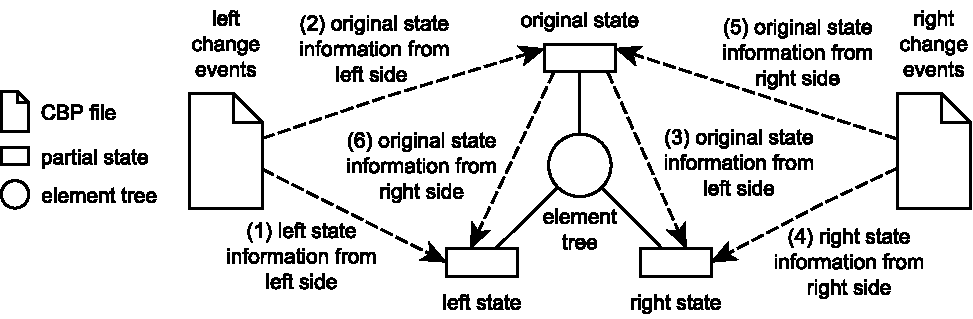
\includegraphics[width=0.8\linewidth]{TreeConstruction}
\caption{Steps in Element Tree construction.}
\label{fig:tree_construction}
\end{figure*} 

\subsubsection{Construction Procedure}\label{sec:construction_procedure}
The construction of \textsf{elementTree} that has been explained follows the steps shown in Figure \ref{fig:tree_construction}. First, the partial
state $S_{L}$ of the left model in the \textsf{elementTree} is constructed based on the information retrieved from the left change events (step 1). We denote this information as $I_{LL}$. We can also construct the partial 
state $S_{O}$ of the original model using the information related to the original state contained in the left change events $I_{OL}$ (step 2). The information $I_{OL}$ allows us to construct the initial partial 
state $S_{R}$ of the right model 
(step 3). Similarly, using the information from the right change events $I_{RR}$, we update the partial right state $S_{R}$ that has been initialised before using the information $I_{OL}$ (step 4), implying that $I_{OL} \cup I_{RR} \rightarrow S_{R}$. Also, information related to the state of the original model from the right change events $I_{OR}$ is used to update the original state  (step 5). Thus, we have a partial state of the original model constructed using information from both left and right sides, $I_{OL} \cup I_{OR} \rightarrow S_{O}$. Finally, we also use the information $I_{OR}$ to update the partial state of the left model (step 6), implying that $I_{LL} \cup I_{OR} \rightarrow S_{L}$.  

Algorithm \ref{alg:element_tree} describes the steps presented in Figure \ref{fig:tree_construction} in a generic fashion. It iterates through all of a model's change events and uses the information contained in them to construct the relevant partial state. The selection of side, left or right change events, that are executed first depends on the \textsf{Side} enumeration value -- \textsf{left} or \textsf{right} -- passed through the parameter \textsf{side} (the second input parameter). In our implementation, we process the left side first by default. The algorithm also receives an input of the change events \textsf{events} that are to be iterated and the element tree \textsf{elementTree} that has been instantiated before and then returns the \textsf{elementTree} as output after updating it.

For each \textsf{event}, we collect information needed to build up \textsf{elementTree}  (lines 3-9), such as \textsf{targetElement}, \textsf{feature}, \textsf{value}, \textsf{previousValue}, \textsf{index}, and \textsf{previousIndex}. The \textsf{targetElement} is the element modified by a change event (e.g., \textsf{character} and \textsf{giant} in Listing \ref{lst:cbp_left}). This \textsf{targetElement} -- an instance of class Element in Figure \ref{fig:approach_class_diagram} -- is retrieved from the \textsf{elementTree} if it already exists. Otherwise, a new element is created and added to the \textsf{elementTree} (line 3). In this step we also set the flags \textsf{*IsCreated} and \textsf{*IsDeleted} of the element in Figure \ref{fig:approach_class_diagram}. For example, if the type of the event is \textsf{create} then \textsf{*IsCreated} is set to \textsf{true}. The \textsf{feature} -- an instance of class Feature in Figure \ref{fig:approach_class_diagram} -- represents the target element's feature (e.g., \textsf{name} and \textsf{operations} in Listing \ref{lst:cbp_right}) modified by a change event. It is retrieved from the \textsf{targetElement}'s feature list, and a new one is created and added to the \textsf{targetElement}'s feature list if the feature does exist (line 5). 

\IncMargin{1.5em}
\begin{algorithm*}[]
\SetKwInOut{Input}{input} 
\SetKwInOut{Output}{output}
\Input{a list of ChangeEvent $events$}
\Input{an enumeration of Side $side$}
\Input{an instance of ElementTree $elementTree$}
\Output{an instance of ElementTree $elementTree$}
\SetKwBlock{Beginn}{beginn}{ende}
\Begin{
	\ForEach{$event$ in $events$}{
		$targetElement$ $\leftarrow$ getOrCreateNewTargetElement($event$, $elementTree$)\;
		$feature$ $\leftarrow$ getOrCreateNewFeature($event$, $targetElement$)\;
		$value$ $\leftarrow$ getValue($event$)\;
		$previousValue$ $\leftarrow$ getPreviousValue($event$)\;
		$index$ $\leftarrow$ getIndex($event$)\;
		$previousIndex$ $\leftarrow$ getPreviousIndex($event$)\;
		$featureEventList$ $\leftarrow$ getFeatureEventList($feature$, $side$)\;
		
		\BlankLine
		\tcp{put all values to their proper indexes}
		updateTree($targetElement$, $feature$, $value$, $index$, $side$)\;
		$oldIndexes$ $\leftarrow$ calculateOldIndex($featureEventList$, $previousIndex$, $side$)\;
		\If{\Not isCreated($value$, $side$) \AndA \Not isOldValueSet($feature$, $previousValue$, $previousIndex$, $side$)} {
			setOldValue($feature$, $previousValue$, $oldIndex$, $side$)\;
			$oppositeFeatureEventList$ $\leftarrow$ getOppositeFeatureEventList($feature$, $side$)\;
			$oppositeIndex$ $\leftarrow$ calculateOppositeIndex($oppositeFeatureEventList$, $oldIndex$, $side$)\;
			\If{\Not isDeleted($value$, $side$) \AndA \Not isOppositeSideValueSet($feature$, $value$, $oppositeIndex$, $side$)} {
				setOppositeSideValue($feature$, $value$, $oppositeIndex$, $side$)\;
			}
		}   
		
		addEventToFeatureEventList($event$, $featureEventList$)\;
		
	}
	\Return{$elementTree$}\;
}
\caption{Algorithm to construct an element tree from events.}
\label{alg:element_tree}
\end{algorithm*}
\DecMargin{1.5em}

The \textsf{value} is the value assigned to the feature in a change event (line 5, Algorithm \ref{alg:element_tree}). The \textsf{value} can be of type \textsf{Element} (e.g., element \textsf{leftGen} line \ref{line:cbp_left_36} in Listing \ref{lst:cbp_left}) or a primitive (e.g., the string ``Hero'' at line \ref{line:cbp_left_34} in the Listing \ref{lst:cbp_left}). The \textsf{previousValue} represents the previous value of the modified feature (line 6, Algorithm \ref{alg:element_tree}). The \textsf{previousValue} is not defined if no previous value has been assigned. For \textsf{value} and \textsf{previousValue} with type \textsf{Element}, the elements that they represent are retrieved from the \textsf{elementTree}, and if they do not exist, new instances are created. If the type is primitive, the value is treated as it is. Not every change event has a \textsf{value}, particularly events with type \textsf{create} 
or \textsf{delete} which only modify a target element not the element's feature.

The \textsf{index} is the index assigned by a change event to a value in a feature, while \textsf{previousIndex} is the previous index of the value (lines 7-8, Algorithm \ref{alg:element_tree}). In one change event, we can get both \textsf{index} and \textsf{previousIndex} or only one of them depending on the type of the change event. For example, we can obtain that the \textsf{index} of \textsf{cast} is 0 (line \ref{line:cbp_right_35} in Listing \ref{lst:cbp_right}) as the change event type is \textsf{add}. In a \textsf{remove} change event, we can only get the \textsf{previousIndex} of \textsf{cast}, that is 1 (line \ref{line:cbp_right_35} in Listing \ref{lst:cbp_right}), as the element does not exist anymore in the left model. We can obtain both of them only in a \textsf{move} change event as an element is moved from a previous index to a new one (line \ref{line:cbp_right_31} in Listing \ref{lst:cbp_right}). For a single-valued feature, the \textsf{index} and \textsf{previousIndex} are always 0 as the feature can only contain a single value. 

At line 9, we retrieve the \textsf{featureEventList} from the \textsf{feature} to be added later with the current \textsf{event} (line 19). The \textsf{featureEventList} is a list -- a history -- of change events that have been processed that are specific to the \textsf{feature} on the selected \textsf{side}. Using the obtained \textsf{targetElement}, \textsf{feature}, \textsf{value}, and \textsf{index}, the process then updates the state of the \textsf{elementTree} on the selected \textsf{side} (line 10). After that, it calculates back the original index of a value using the \textsf{featureEventList} and \textsf{previousIndex} (line 11). If the value at \textsf{oldIndex} in the \textsf{feature} has not been set, then the algorithm sets the \textsf{feature} with the \textsf{previousValue} at the \textsf{oldIndex} in the partial state of the original model (lines 12-13). At lines 14-18, the algorithm also does the same thing to the opposite side.

\subsubsection{Change Event Mapping}
\label{sec:change_event_mapping}
Using the information contained in the change-based model representations in Listings \ref{lst:cbp_left} and \ref{lst:cbp_right}, we can construct an element tree as depicted in Figure \ref{fig:right_element_tree_diagram} using the construction method presented in Section \ref{sec:tree_construction}. During the the construction, change events in Listings \ref{lst:cbp_left} and \ref{lst:cbp_right} are mapped to the affected elements, features, and values which act as the keys of the mapping. The relationships are stored in attributes \textsf{leftEvents} and \textsf{rightEvents} of class \textsf{Element} and \textsf{leftEvents}, \textsf{rightEvents}, \textsf{leftValueEvents}, and \textsf{rightValueEvents} of class \textsf{Feature} in Figure \ref{fig:approach_class_diagram}. This registration forms many-to-many relationships between the keys and change events. In detail, the keys are \textsf{element} for elements, or a combination of \textsf{element-feature} for single-valued features or \textsf{element-feature-value} for multivalued-features. With this mapping, we can trace all events that affects certain elements, features, and values. The mapping of the events in Listings \ref{lst:cbp_left} and \ref{lst:cbp_right} is in Table \ref{tab:keyeventsmap}. The application of this mapping is presented in Section \ref{sec:delete_conflict}.

\begin{table}[ht]
\centering
\caption{The mapping of elements, features, and values in Figure \ref{fig:right_element_tree_diagram} to the events that affect them.}
\label{tab:keyeventsmap}
\begin{sffamily}
	\begin{tabular}{|m{0.36\linewidth}|m{0.245\linewidth}|m{0.245\linewidth}|}
		\hline
		\textbf{Key} & \textbf{Left Events} & \textbf{Right Events} \\ \hline
		character                          & cl32, cl34                                & cr37, cr39                                 \\ \hline
		character.name                     & cl34                                      & cr39                                       \\ \hline
		attack                             & cl37                                      & cr31                                       \\ \hline
		attack.parameters.target           & cl37                                      & cr31                                       \\ \hline
		target                             & cl37                                      & cr31                                       \\ \hline
		trcll                              & cl33, cl35                                & cr38, cr40                                 \\ \hline
		trcll.name                         & cl43                                      & cr42                                       \\ \hline
		trcll.generalization               & cl33, cl35                                & cr38, cr40                                 \\ \hline
		giant                              & cl39, cl40, cl41, cl42                    & cr33, cr34                                 \\ \hline
		giant.name                         & cl40                                      &                                            \\ \hline
		giant.operations.cast              & cl39                                      & cr34                                       \\ \hline
		giant.operations.smash             &                                           & cr33                                       \\ \hline
		knight                             & cl36                                      & cr32                                       \\ \hline
		knight.generalization              & cl36                                      &                                            \\ \hline
		knight.operations.smash            &                                           & cr32                                       \\ \hline
		mage                               &                                           & cr35, cr41                                 \\ \hline
		mage.generalization                &                                           & cr41                                       \\ \hline
		mage.operations.cast               &                                           & cr35                                       \\ \hline
		leftGen                            & cl31, cl32, cl33, cl35, cl36              &                                            \\ \hline
		leftGen.general                    & cl32                                      &                                            \\ \hline
		rightGen                           &                                           & cr36, cr37, cr38, cr40, cr41               \\ \hline
		rightGen.general                   &                                           & cr37                                       \\ \hline
		smash                              &                                           & cr32, cr33                                 \\ \hline
		cast                               & cl38, cl39, cl40                          & cr34, cr35                                 \\ \hline
		cast.name                          & cl38                                      &                                            \\ \hline
	\end{tabular}\\
\end{sffamily}
c: change event; l: left side; r: right side; n: line number in change-based model persistence
\end{table}

\subsection{Conflict Computation} 
\label{sec:conflict_computation} 
This section explains how the information contained in the \textsf{elementTree} is used to detect conflicts between two versions of a model. First, we discuss the theoretical foundation of the conflict detection approach. After that, we explain detecting conflicts related to deletion of an element, cross-containment movement, singe-valued feature, and ordered/unordered multi-valued feature. 

\subsubsection{Theoretical Foundation} 
\label{sec:theoretical_foundation}
In the proposed conflict detection approach, we take two strategies from both change and state-based conflict detections to improve the accuracy of our approach. 
First, we exploit change events to accurately address real historical changes -- not derived ones -- of models. Second, we also take into account the original and eventual states of the modified models. Two sequences of change events that produce two eventual states that are equal to an original state are not treated as in conflict. The original and eventual states are already calculated during the construction of the \textsf{element tree} so that we do not need to calculate them again in the conflict computation phase. Since all change events are also recorded for every element, feature, and value that they affected, we can retrieve all related change events that produce the eventual state of an element or feature. 

Let’s say that we have the original state of an element $e_{o}$. We also have a list of change events $C_{L}$ = $(c_{l1}$, $c_{l2}$, ..., $c_{lg})$ that we apply to $e_{o}$ to change its state to element $e_{l}$ and $g = |C_{L}|$.
\begin{equation} \label{eq:ecbp_left}
e_{o} + c_{l1} + c_{l2} + ... + c_{lg} \rightarrow e_{l}
\end{equation}
We also have a list of change events $C_{R}$ = $(c_{r1}$, $c_{r2}$, ..., $c_{rh})$ that we apply to $e_{o}$ to produce element $e_{r}$ and $h = |C_{R}|$.
\begin{equation} \label{eq:ecbp_right}
e_{o} + c_{r1} + c_{r2} + ... + c_{rh} \rightarrow e_{r}
\end{equation}
\textbf{Non-conflict}. Instead of calculating conflict between change events, we start by checking the equivalence of the left and right states of an element to its original state. If the states of both sides are equivalent to the original state, regardless of how many changes have been applied, we can infer that there is no conflict between the members of the two change event lists, $C_{L}$ and $C_{R}$, since there is no change of the eventual state. We also identify no conflict if an element is modified only on one side—no change events are applied on the other side.
\begin{equation} \label{eq:ecbp_nonconflict}
\begin{split}
	& (e_{o} \equiv e_{l} \wedge e_{o} \equiv e_{r}) \vee |C_{L}| = 0 \vee |C_{R}| = 0 \Rightarrow\\
	& \neg(c_{l} \;!\; c_{r}) \;|\; c_{l} \in C_{L}, c_{r} \in C_{R}
\end{split}
\end{equation}
\textbf{Conflict}. A conflict occurs when one or both states, $e_{l}$ or/and $e_{r}$, are not equivalent to the original state $e_{o}$, and there is at least one change event applied on each side of the element. We can conclude that change event list $C_{L}$ is in conflict with the change event list $C_{R}$.
\begin{equation} \label{eq:ecbp_conflict}
\begin{split}
	& (e_{o} \not\equiv e_{l} \vee e_{o} \not\equiv e_{r}) \wedge (|C_{L}| > 0 \wedge |C_{R}| > 0) \Rightarrow\\
	& c_{l} \;!\; c_{r} \;|\; c_{l} \in C_{L}, c_{r} \in C_{R}
\end{split}
\end{equation}
\textbf{Pseudo-conflict}. As in EMF Compare, we also implement pseudo conflict. Pseudo conflict is a conflict where $e_{l}$ and $e_{r}$ are equivalent or one of them is equivalent to $e_{o}$ thus they can be automatically resolved in conflict resolution without user intervention.
\begin{equation} \label{eq:ecbp_pseudoconflict}
\begin{split}
	(& e_{o} \equiv e_{l} \vee e_{o} \equiv e_{r} \vee e_{l} \equiv e_{r}) \wedge (|C_{L}| > 0 \wedge |C_{R}| > 0)\\
	& \Rightarrow \forall c_{l} \;!_{p}\; \forall c_{r} \;|\; c_{l} \in C_{L}, c_{r} \in C_{R}
\end{split}
\end{equation} 

Figure \ref{fig:conflict_states} are some examples how conflict and non-conflict change events are detected in the proposed approach (dashed arrow = left change event, solid arrow = right change events, circle = state). Figure \ref{fig:statechart_01} shows the initial state of an element is `a'. In the figure, the element has not been modified. Thus, no conflict is detected according to (\ref{eq:ecbp_nonconflict}). In Figure \ref{fig:statechart_02}, the element is modified on the right side (version) only. Thus, using (\ref{eq:ecbp_nonconflict}), no conflict is detected. In the figure, the state of the element is altered from `a' to `b' by change event $cr1$, and then altered again to `c' by change event $cr2$. In Figure \ref{fig:statechart_03}, even though an element has been modified on both sides, using (\ref{eq:ecbp_nonconflict}), no conflict is detected, since both left and right states are equal to the original state after the modification. In the figure, both $C_{L}$ and $C_{R}$ produces eventual states that are equal to the original state, `a'. 

\begin{figure}[ht]
\begin{subfigure}[t]{0.48\linewidth}
	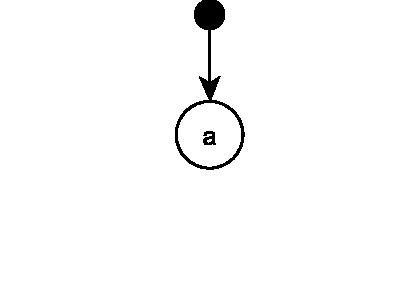
\includegraphics[width=\linewidth]{statechart_01}
	\caption{non-conflict}
	\label{fig:statechart_01}
\end{subfigure}
\hfill
\begin{subfigure}[t]{0.48\linewidth}
	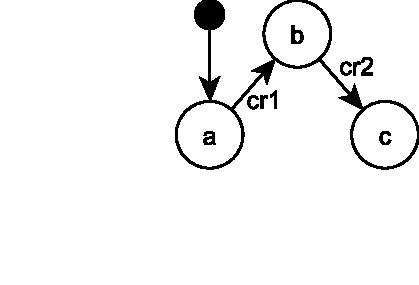
\includegraphics[width=\linewidth]{statechart_02}
	\caption{non-conflict}
	\label{fig:statechart_02}
\end{subfigure}
\\
\begin{subfigure}[t]{0.48\linewidth}
	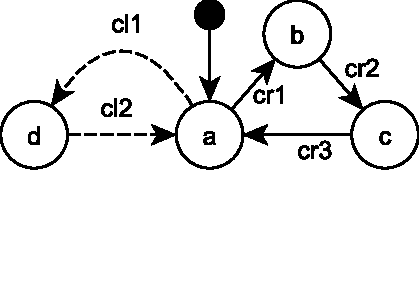
\includegraphics[width=\linewidth]{statechart_03}
	\caption{non-conflict}
	\label{fig:statechart_03}
\end{subfigure}
\hfill
\begin{subfigure}[t]{0.48\linewidth}
	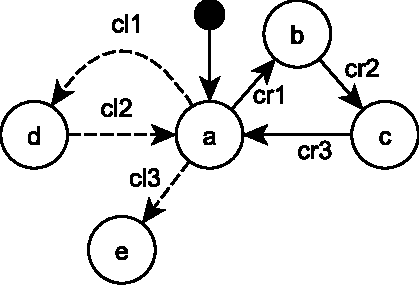
\includegraphics[width=\linewidth]{statechart_04}
	\caption{pseudo-conflict}
	\label{fig:statechart_04}
\end{subfigure}
\\
\begin{subfigure}[t]{0.48\linewidth}
	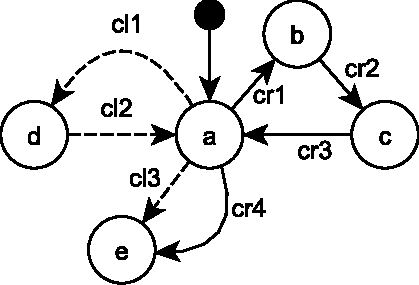
\includegraphics[width=\linewidth]{statechart_05}
	\caption{pseudo-conflict}
	\label{fig:statechart_05}
\end{subfigure}
\hfill
\begin{subfigure}[t]{0.48\linewidth}
	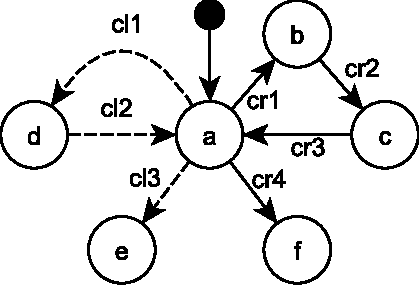
\includegraphics[width=\linewidth]{statechart_06}
	\caption{conflict}
	\label{fig:statechart_06}
\end{subfigure}
\caption{Conflicting and non-conflicting change events (dashed arrow = left change event, solid arrow = right change events, circle = state).}
\label{fig:conflict_states}
\end{figure}

Using (\ref{eq:ecbp_pseudoconflict}), the condition in Figure \ref{fig:statechart_04} can be detected as a \textsf{PSEUDO} conflict. \textsf{PSEUDO} conflict means that a conflict can be automatically resolved. This means that we can automatically select one of the two conflicting change event lists as the applied change events without needing human intervention. Since $C_{R}$ produces the eventual state that is equal to the original state, that is, ‘a’; it does not have any effect—the changes are not intended or cancelled. Thus, all its change events can be automatically negated. In other words, only the change events in $C_{L}$ are accepted to produce the eventual state, which is ‘e’. Also using (\ref{eq:ecbp_pseudoconflict}), the condition in \ref{fig:statechart_05} can be detected as another \textsf{PSEUDO} conflict. Both change event lists, $C_{L}$ and $C_{R}$, produce the same eventual state, ‘e’, that is different from the original state, ‘a’. This can be automatically resolved since selecting either one of the lists produces the same outcome. With (\ref{eq:ecbp_conflict}), the scenario in Figure \ref{fig:statechart_06} can be detected as a \textsf{REAL} conflict, since change event lists, $C_{L}$ and $C_{R}$, produce two different eventual states. The conflict cannot be automatically resolved, and it requires user intervention to choose which one is the desired eventual state, ‘e’ or ‘f’. Then the appropriate change event list can be selected to produce the eventual state.

We perform procedure in Algorithm \ref{alg:conflict_detection} and employ (\ref{eq:ecbp_conflict}) and (\ref{eq:ecbp_pseudoconflict}) inside it to identify conflicts between two CBPs. Essentially, the algorithm works by iterating through all the elements, features, and values in the element tree  (Figure \ref{fig:right_element_tree_diagram}) and checking the equivalency of their original and eventual states as well the numbers of change events applied to them. The results are then used as inputs to decide whether a conflict has been detected or not.

\begin{table*}[ht]
\centering
\caption{Conflicting change events in Listings \ref{lst:cbp_left} and \ref{lst:cbp_right} identified using the proposed change-based conflict detection. The bold identifiers are the keys where the conflicts detected.}
\label{table:conflicts_cbp}
\begin{tabular}{|p{0.04\linewidth}|p{0.38\linewidth}|p{0.38\linewidth}|
		p{0.1\linewidth}|}
	\hline
	\textbf{ID} & 
	\textbf{Left Change Events (Bob)} & 
	\textbf{Right Change Events (Alice)} & 
	\textbf{Type}\\ 
	\hline
	CB1 & 
	set \textbf{troll.name} from "Troll" to "Ogre" & 
	set \textbf{troll.name} from "Troll" to "Orc" & 
	real \\
	\hline
	CB2 & move \textbf{target} in \textbf{character.parameters} from 1 to 2 & 
	move \textbf{target} in \textbf{character.parameters} from 1 to 0 & 
	real \\ 
	\hline
	CB3 & 
	\begin{minipage}[t]{\linewidth}
		\raggedright
		\begin{itemize}[leftmargin=0pt]
			\setlength
			\item[] unset cast.name from "cast" to null
			\item[] remove cast from giant.operations at 0
			\item[] delete cast type Operation
			\item[] unset giant.name from "Giant" to null
			\item[] delete \textbf{giant} type Class
		\end{itemize}
	\end{minipage}
	& 
	\begin{minipage}[t]{\linewidth}
		\raggedright
		\begin{itemize}[leftmargin=0pt]
			\setlength
			\item[] remove smash from knight.operations at 0
			\item[] add smash to \textbf{giant}.operations at 1
			\item[] remove cast from \textbf{giant}.operations at 0
			\item[] add cast to mage.operations at 0
		\end{itemize}
	\end{minipage}
	& 
	real, non-applicability\\
	\hline
	CB4 & 
	\begin{minipage}[t]{\linewidth}
		\raggedright
		\begin{itemize}[leftmargin=0pt]
			\setlength
			\item[] unset cast.name from "cast" to null
			\item[] remove cast from giant.operations at 0
			\item[] delete \textbf{cast} type Operation
			\item[] unset giant.name from "Giant" to null
			\item[] delete giant type Class
		\end{itemize}
	\end{minipage}
	& 
	\begin{minipage}[t]{\linewidth}
		\raggedright
		\begin{itemize}[leftmargin=0pt]
			\setlength
			\item[] remove \textbf{cast} from giant.operations at 0
			\item[] add \textbf{cast} to mage.operations at 0
		\end{itemize}
	\end{minipage}
	& 
	real, non-applicability\\
	\hline
	CB5 & 
	set \textbf{character.name} from "Character" to "Hero" & 
	set \textbf{character.name} from "Character" to "Hero" & 
	pseudo\\ 
	\hline
\end{tabular}
\end{table*}

%------------------------------------------------------------------------------

The algorithm starts by creating an empty list \textsf{conflictList} to contain identified conflicts at line 2. The algorithm then iterates through all the elements, features, and values in the element tree. 

\subsubsection{Conflict with Deletion} 
\label{sec:delete_conflict} 
At lines 4 to 11 in Algorithm \ref{alg:conflict_detection}, the algorithm checks if there is a conflict related to a deletion of an element.
If an element is deleted on one or both sides, it means that all events related to that element on both sides should be in conflict.
The algorithm uses two functions, \textsf{getAllRelatedLeftEvents($element$)} and \textsf{getAllRelatedRightEvents($element$)}, to get all the related events (the element acts as a map key to access the change events). These functions return two lists of related events,
\textsf{leftEvents} and \textsf{rightEvents} respectively. The related events are events applied to the deleted element, including its sub-elements and features,
and events that are part of composite events. If both lists of events are not empty, then a conflict is created containing both lists of events.
If the element is deleted on both sides, then we set the conflict as \textsf{PSEUDO}. The identified conflict is then added to \textsf{conflictList}.

\IncMargin{1.5em}
\begin{algorithm*}[]
\SetKwInOut{Input}{input}
\SetKwInOut{Output}{output}
\Input{an instance of ElementTree $elementTree$}
\Begin{
	$conflictList$ $\leftarrow$ ConflictList()\;
	\ForEach{$element$ \In $elementTree$}{
		\tcp{Handle conflicts with deletion ----------------------------}
		\If{isLeftDeleted($element$) \Or isRightDeleted($element$)}{
			$leftEvents$ $\leftarrow$ getAllRelatedLeftEvents($element$)\;
			$rightEvents$ $\leftarrow$ getAllRelatedRightEvents($element$)\;
			\If{size($leftEvents$) > 0 \AndA size($rightEvents$) > 0}{
				$conflict$ $\leftarrow$ createConflict($leftEvents$, $rightEvents$)\;
				\If{isLeftDeleted($element$) \AndA isRightDeleted($element$)}{
					setPseudo($conflict$)\;
				}
				addConflict($conflict$, $conflictList$)\;
				continue\;
			}
		}
		\tcp{Handle conflicts with cross-container move --------------------------}
		\If{(getOriginalContainer($element$) <> getLeftContainer($element$) \Or getOriginalContainingFeature($element$) <> getLeftContainingFeature($element$)) \Or
			(getOriginalContainer($element$) <> getRightContainer($element$) \Or getOriginalContainingFeature($element$) <> getRightContainingFeature($element$))}{
			$leftEvents$ $\leftarrow$ getAllRelatedLeftEvents($element$)\;
			$rightEvents$ $\leftarrow$ getAllRelatedRightEvents($element$)\;
			\If{size($leftEvents$) > 0 \AndA size($rightEvents$) > 0}{
				$conflict$ $\leftarrow$ createConflict($leftEvents$, $rightEvents$)\;
				\If{getLeftContainer($element$) = getRightContainer($element$) \AndA getLeftContainingFeature($element$) = getRightContainingFeature($element$}{
					setPseudo($conflict$)\;
				}
				addConflict($conflict$, $conflictList$)\;
			}
		}
		\ForEach{$feature$ \In getFeatures($element$)}{
			\tcp{Handle single-valued feature}
			handleSingleValuedFeature($element$, $feature$, $conflictList$)\;\label{line:conflict_single_value}
			\tcp{Handle multi-valued feature} 
			handleMultiValuedFeature($element$, $feature$, $conflictList$)\;\label{line:conflict_multi_value}
		}
	}
	\Return{$conflictList$}\;
}
\caption{Algorithm for conflict detection using element tree.}
\label{alg:conflict_detection}
\end{algorithm*}
\DecMargin{1.5em}

As an example, when the iteration reaches element \textsf{giant} in Figure \ref{fig:right_element_tree_diagram}, the algorithm identifies that the element has been deleted only on the left side.
Using the map in Table \ref{tab:keyeventsmap}, the algorithm then collects all the change events from both sides related to the element \textsf{giant} and its sub-elements. For key \textsf{giant}, it collects the change events at lines 39 to 42 for the left side and change events at lines 33 to 34 for the right side. For key \textsf{giant.name}, only left-side change event at line 40 is collected.
For key \textsf{giant.operations.cast}, it collects left-side change event at line 39 and right-side change event at line 34.
For key \textsf{giant.operations.smash}, only the right-side change event at line 33 is collected. 
For key \textsf{cast}, it collects change events at lines 38 to 40 for the left side and change events at lines 34 and 35 for the right side.
For key \textsf{giant.name}, it only left-side change event at line 38 is collected.
The collected change events are merged into one list of change events for each side. 
So, the left events are all events that comprise the composite event that deletes the element. 
The right events consist of events that move operation \textsf{smash} from class \textsf{knight} to class \textsf{giant} and events that
move operation \textsf{cast} from class \textsf{giant} to class \textsf{mage}. The algorithm then creates a conflict that consists of these events 
producing conflict \textsf{CB3} in Table \ref{table:conflicts_cbp}. 

When the iteration reaches element \textsf{cast} -- the operation of class \textsf{giant}, the same procedure is repeated. It collects left-side change events at lines 33, 38, 39, 40, 41, and 42, and right-side change events at lines 34, 35, and 38. The left-side change events related to element \textsf{giant} are also included since they are in one composite event that also affects element \textsf{cast}. These change events are collected into one conflict, \textsf{CB4}. 

It can be noticed that both conflicts \textsf{CB3} and \textsf{CB4} have shared change events. Thus these conflicts have a dependency on each other. It means that if a user chooses to delete \textsf{giant} -- choose the left side as the solution -- for conflict \textsf{CB3}, the left side change events also have to be selected as the solution for conflict \textsf{CB4} for consistency. To facilitate computing such dependencies, conflicts and change events are designed to have many-to-many relationships as depicted in Figure \ref{fig:approach_class_diagram}. Thus, if a change event is associated with two or more conflicts, it means that they depend on each other.

It is important to notice that at line 13 in Figure \ref{alg:conflict_detection} there is a command \textsf{continue} after the addition of a conflict caused by deletion. The command skips the iteration to the next element which avoids unnecessary conflict computation for the current element's  features and values. All change events related to the features and values have been collected by the functions \textsf{getAllRelatedLeftEvents($element$)} and \textsf{getAllRelatedRightEvents($element$)} at lines 5 and 6.  

\subsubsection{Conflict between Cross-container Moves} 
\label{sec:move_conflict} 
Lines 15 to 25 in Algorithm \ref{alg:conflict_detection} are dedicated to identifying conflicts related to cross-container moves. 
First, the algorithm checks if an element has been moved from its original container to another container on one or both sides. 
If it does has been moved, 
it then checks the number of events related to the element by firstly obtaining change events related to the element on 
both sides using functions \textsf{getAllRelatedLeftEvents($element$)} and \textsf{getAllRelatedLeftEvents($element$)} yielding two lists of events, 
\textsf{leftEvents} and \textsf{rightEvents}. If the element has, at least, one event on each side,
a conflict is created containing \textsf{leftEvents} and \textsf{rightEvents}. 
If on both sides the element is moved to the same container, or the element is moved but finally returns to its original container on one of its sides, then the conflict is set to \textsf{PSEUDO}.

\IncMargin{1.5em}
\begin{algorithm*}[]
\SetKwInOut{Input}{input}
\SetKwInOut{Output}{output}
\Input{an element $element$}
\Input{a feature $feature$}
\Input{a list to contain conflicts $conflictList$}
\Begin{
	\tcp{Handle single-valued feature --------------------------}
	\If{isSingleValued($feature$)}{
		$originalValue$ $\leftarrow$ getOriginalValue($feature$)\;
		$leftValue$ $\leftarrow$ getLeftValue($feature$)\;
		$rightValue$ $\leftarrow$ getRightValue($feature$)\;
		$leftEvents$ $\leftarrow$ getAllRelatedLeftEvents($element$, $feature$)\;
		$rightEvents$ $\leftarrow$ getAllRelatedRightEvents($element$, $feature$)\;
		\If{$originalValue$ <> $leftValue$ \Or $originalValue$ <> $rightValue$ \AndA size($leftEvents$) > 0 \AndA size($rightEvents$) > 0}{
			$conflict$ $\leftarrow$ createConflict($leftEvents$, $rightEvents$)\;
			\If{$leftValue$ = $rightValue$ \Or $leftValue$ = $originalValue$ \Or $rightValue$ = $originalValue$}{
				setPseudo($conflict$)\;
			}
			addConflict($conflict$, $conflictList$)\;
		}
	}
}
\caption{Algorithm to handle single-valued feature in conflict detection using element tree -- handleSingleValuedFeature($element$, $feature$, $conflictList$) at line 27 in Algorithm \ref{alg:conflict_detection}.}
\label{alg:conflict_single_valued_feature}
\end{algorithm*}
\DecMargin{1.5em}

\subsubsection{Single-valued Feature Conflict} 
\label{sec:single_valued_conflict}
Conflicts that involve single-valued features are handled by the procedure at line \ref{line:conflict_single_value} in Algorithm \ref{alg:conflict_detection}, which is elaborated in Algorithm \ref{alg:conflict_single_valued_feature}. The procedure starts by retrieving \textsf{leftValue}, \textsf{rightValue}, and \textsf{originalValue} of a single-valued feature. It then checks the inequality of \textsf{leftValue} and \textsf{rightValue} to \textsf{originalValue}. If either \textsf{leftValue} or \textsf{rightValue} is not equal to \textsf{originalValue}, it continues to check the number of change events related to the feature by retrieving them using functions \textsf{getAllRelatedEvents($element$, $feature$)} and \textsf{getAllRelatedRightEvents($element$, $feature$)} (element and feature act as map keys to access the events). This yields two lists of related events, \textsf{leftEvents} and \textsf{rightEvents}. If \textsf{leftEvents} and \textsf{rightEvents} are not empty, then a conflict that contains these events is instantiated. The procedure then checks whether \textsf{leftValue} and \textsf{rightValue} are equal, and it sets the conflict to \textsf{PSEUDO} if \textsf{leftValue} and \textsf{rightValue} are equal to each other or if one of them is equal to \textsf{originalValue}. Finally, the conflict is put into \textsf{conflictList}.

For example, when the iteration reaches feature \textsf{name} of class \textsf{troll}, the algorithm retrieves the left, right, and original values of the feature, yielding “Ogre”, “Orc”, and “Troll”, respectively. Since “Ogre” and “Orc” are not equal to “Troll’, the algorithm continues to retrieve two lists of events related to the feature. Only one event contained exists in each list. On the left side, the event sets the name of class \textsf{troll} from “Troll” to “Ogre”, while on the right side, the event sets it from “Troll” to “Orc”. Both event sets are not empty. Thus, a conflict containing them is created. Since “Ogre” is not equal to “Orc”, the conflict is not set to \textsf{PSEUDO}. This conflict is the conflict \textsf{CB1} in Table \ref{table:conflicts_cbp}. This part of the algorithm also identifies conflict \textsf{CB5}, except that this conflict is set to \textsf{PSEUDO} since both sides change class \textsf{character}’s \text{name} to the same value, “Hero”. 

\subsubsection{Ordered Multi-valued Feature Conflict} 
\label{sec:ordered_conflict}
Conflicts that involve multi-valued features are handled by the procedure at line \ref{line:conflict_multi_value} in Algorithm \ref{alg:conflict_detection}. The procedure is elaborated in Algorithm \ref{alg:conflict_multi_valued_feature}, where ordered multi-valued features are addressed at lines 3–15. The procedure relies on the function \textsf{getUnequalLeftAndRightValues}. This function returns all values from left and right sides that are not equal to their original states in terms of (in)existence and indexes. For example, in Figure \ref{fig:right_element_tree_diagram}, parameter \textsf{target} in feature \textsf{parameters} is at index 2 on the left side but at index 1 in its original state. Thus, the value is included in the returned list. On the right side, this parameter is also at an index different from its original index, but it is already included in the returned list.

\IncMargin{1.5em}
\begin{algorithm*}[]
\SetKwInOut{Input}{input}
\SetKwInOut{Output}{output}
\Input{an element $element$}
\Input{a feature $feature$}
\Input{a list to contain conflicts $conflictList$}
\Begin{
	\tcp{Handle multi-valued feature --------------------------}
	\If{isMultiValued($feature$)}{
		\uIf{isOrdered($feature$)}{
			$values$ $\leftarrow$ getUnequalLeftAndRightValues($feature$)\;
			\ForEach{$value$ \In $values$}{
				$leftEvents$ $\leftarrow$ getAllRelatedLeftEvents($element$, $feature$, $value$)\;
				$rightEvents$ $\leftarrow$ getAllRelatedRightEvents($element$, $feature$, $value$)\;
				\If{size($leftEvents$) > 0 \AndA size($rightEvents$) > 0}{
					$conflict$ $\leftarrow$ createConflict($leftEvents$, $rightEvents$)\;
					\If{getLeftIndex($value$, $feature$) = getRightIndex($rightValue$, $feature$) \Or getLeftIndex($value$, $feature$) = getOriginalIndex($value$, $feature$) \Or getRightIndex($value$, $feature$) = getOriginalIndex($value$, $feature$)}{
						setPseudo($conflict$)\;
					}
					addConflict($conflict$, $conflictList$)\;
				}       
			}
		}\ElseIf{\Not isOrdered($feature$)}{
			$leftValues$ $\leftarrow$ getXORLeftAndOriginalValues($feature$)\;
			$rightValues$ $\leftarrow$ getXORRightAndOriginalValues($feature$)\;
			$values$ $\leftarrow$ $leftValues$ $\cup$ $rightValues$\;
			\ForEach{$value$ \In $values$}{
				$leftEvents$ $\leftarrow$ getAllRelatedLeftEvents($element$, $feature$, $value$)\;
				$rightEvents$ $\leftarrow$ getAllRelatedRightEvents($element$, $feature$, $value$)\;
				\If{size($leftEvents$) > 0 \AndA size($rightEvents$) > 0}{
					$conflict$ $\leftarrow$ createConflict($leftEvents$, $rightEvents$)\;
					\If{isLeftExisted($value$, $feature$) = isRightExisted($value$, $feature$) \Or isLeftExisted($value$, $feature$) = isOriginExisted($value$, $feature$) \Or isRightExisted($value$, $feature$) = isOriginExisted($value$, $feature$)}{
						setPseudo($conflict$)\;
					}
					addConflict($conflict$, $conflictList$)\;
				}       
			}
		}
	}
}
\caption{Algorithm to handle multi-valued feature in conflict detection using element tree -- handleMultiValuedFeature($element$, $feature$, $conflictList$) at line 28 in Algorithm \ref{alg:conflict_detection}.}
\label{alg:conflict_multi_valued_feature}
\end{algorithm*}
\DecMargin{1.5em}

The algorithm then iterates through the values of the list. For each value, it retrieves all events related to the value of this feature. (Element, feature, and value act as map keys to access the events.) The algorithm uses function \textsf{getAllRelated *Events($element$, $feature$, $value$)}, which yields two lists of events, \textsf{leftEvents} and \textsf{rightEvents}. If both lists of events are not empty, then a conflict is created. If the value on both sides is at the same index, then the conflict is \textsf{PSEUDO}. Finally, the conflict is added to \textsf{conflictList}. The parameter \textsf{target} in feature \textsf{parameters} has been concurrently modified; it has one event on each side: parameter \textsf{target} is moved to the last index on the left side and to the first index on the right. Thus, a conflict is detected. This conflict is presented as conflict \textsf{CB2} in Table \ref{table:conflicts_cbp}.

%\begin{figure}[ht]
%    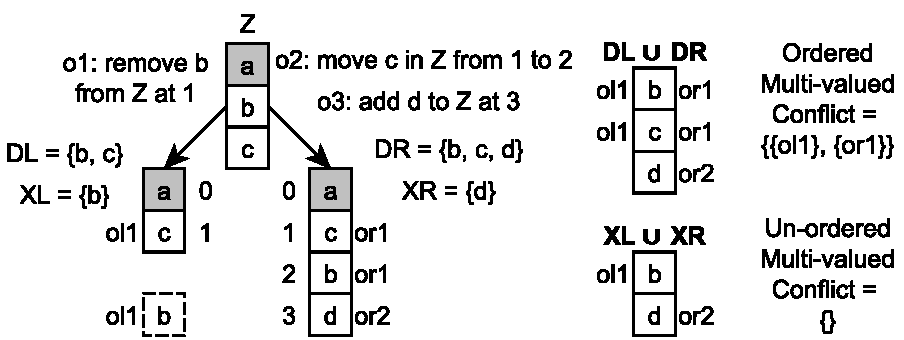
\includegraphics[width=\linewidth]{multi_valued_conflict_detection}
%    \caption{Detecting conflicts in Multi-valued features ($D$: values that are different at every index; $X$: XOR of values).}
%    \label{fig:multi_valued_conflict_detection}
%\end{figure}

\subsubsection{Unordered Multi-valued Feature Conflict} 
\label{sec:unordered_conflict}
Conflict detection for unordered, multi-valued features is handled at lines 16 to 29 in Algorithm \ref{alg:conflict_multi_valued_feature}. Instead of using function \textsf{getUnequalLeftAndRightValues}, it employs \textsf{getXOR*AndOriginalValues} functions. The functions also return all values from left and right sides that are not equal to their original states but only in terms of (in)existence since indexing is not important in un-ordered features. The procedure to detect a conflict is similar to the procedure for ordered features. The difference is that to determine if a conflict is \textsf{PSEUDO} or not, it checks the existence of values using functions \textsf{is*Existed}.

\section{Algorithm Complexity}
\label{sec:conflict_algorithm_complexity}
The algorithm of state-based model conflict detection consists of two steps. The first step derives two lists of changes from two compared versions and their common original version, and the second step determines conflicting changes from the two lists. In the first step, the time and space complexity is \textsf{2ND}: \textsf{N} is the sum of the lengths of two compared sequences, \textsf{D} is the size of the minimum edit script for both sequences \cite{DBLP:journals/algorithmica/Meyers86}, and \textsf{2} is for performing state-based model differencing twice; differencing between the left and original versions and the right and original versions. In the second step, the time complexity is \textsf{E} which is the number of elements, features, and values that are different in the left and right models, and the complexity of space is \textsf{X} which is the number of conflicts detected. So, overall, the time complexity of state-based model conflict detection is \textsf{O}(\textsf{2ND} + \textsf{E}) and its space complexity is \textsf{O}(\textsf{2ND} + \textsf{X)}. Therefore, we can infer that, for time and space complexity, the algorithm works best when differences are small -- sequences are similar -- and worst when the sequences are entirely different.

Change-based model conflict detection follows similar phases to change-based model differencing \cite{yohannis2019efficient}; it also performs event loading (Section \ref{sec:event_loading}) and tree construction (Section \ref{sec:tree_construction}) but replaces the differencing/difference computation with conflict computation (Section \ref{sec:conflict_computation}). Therefore, event loading follows the same time and space complexity as change-based model differencing, which depends on \textsf{C}, the total number of change events loaded from two compared versions. 

In the tree construction, it adds an additional activity that maps change events to the elements, features, and values that they affect (Section \ref{sec:change_event_mapping}). This activity does not change the time and space complexity of tree construction since mapping in hash tables has time complexity of \textsf{O}(\textsf{1}) in average \cite{cormen2009introduction}, and the average space complexity is determined by the number of elements \textsf{O}(\textsf{n}) \cite{cormen2009introduction}. Therefore, we can infer that the mapping does not change the overall time complexity in tree construction, which depends on \textsf{C}, and the space complexity is still defined by \textsf{E}; the number of elements, features, and values affected by change events.  

On the tree, the conflict computation runs linearly by iterating through each affected element, feature, or value and determines their conflicting states caused by change events (Algorithms \ref{alg:conflict_detection}, \ref{alg:conflict_single_valued_feature}, and \ref{alg:conflict_multi_valued_feature}). Its time complexity is \textsf{E} which is the number of affected elements, features, and values that are in conflict. Its space complexity is \textsf{X}, the number of spaces allocated to hold the identified conflicts in memory. 

The time complexity for the proposed change-based model conflict detection is \textsf{O}(\textsf{C} + \textsf{E}) where \textsf{C} is the number of change events that are loaded and executed to construct an element tree, and \textsf{E} is the number of elements, features, and values affected by the changes. Moreover, the space complexity is \textsf{O}(\textsf{C} + \textsf{E} + \textsf{X}) where \textsf{C} corresponds to the number of space to hold all the involved change events in memory, \textsf{E} is the space required to store elements, features, and values of an element tree in memory, and \textsf{X} is the space to store the identified conflicts in memory.

In terms of time complexity, change-based model conflict detection works best in a condition where the number of change events and the number of affected elements, features, and values is small and worst when these numbers are large -- many changes are made, and they affect many parts of a model. 

In terms of space complexity, the best case happens when a model undergoes small changes, limited to certain parts of the model, and the changes produce only a small number of conflicts. In contrast, the worst-case for space complexity happens when a model experiences significant changes, which is indicated by a large number of change events, a large number of affected elements, features, and values (changes are distributed evenly throughout the model), and the two versions produced by the changes are entirely different.

\section{Accuracy of Conflict Detection}
\label{sec:accuracy_of_conflict_detection}
Conflicts detected by EMF CBP, EMF Compare, and EMF Store can be different due to the different approaches employed by them. In this section, we explain in more detail the differences, firstly, between EMF CBP and EMF Compare, and secondly, between EMF CBP and EMF Store, on the conflicts they can/cannot detect. We use this classification of detected/undetected conflicts later in the evaluation to compare the accuracy of these tools.

\subsection{EMF CBP vs. EMF Compare}
\label{sec:emf_cbp_vs_emf_compare}
EMF Compare uses model differencing to derive changes -- not the actual changes -- between two versions of a model. This can cause EMF Compare to treat an element or feature as it has been modified even though no change has been applied to it in the actual context, and further can lead EMF Compare to inaccurate conflict detection. On the other side, EMF CBP uses actual recorded change events to determine conflicts; thus, its conflict detection is accurate. The following is the kinds of conflicts detected by EMF CBP but fail to be detected by EMF Compare. 
\begin{itemize}

\item \emph{Real Move Conflict}. EMF CBP identifies accurately an element that has been moved, but EMF Compare picks another element. This case has been presented in the running example where EMF CBP detects that \textsf{target} has been moved on both sides (Conflict CB2, Table \ref{table:conflicts_cbp}), while EMF Compare identifies \textsf{target} and \textsf{gem} that have been moved on the left and right sides respectively (Listings \ref{lst:cbp_left_state} and \ref{lst:cbp_right_state}).

\item \emph{One-sided Reset Conflict}. EMF CBP detects a \textsf{PSEUDO} conflict on an element or feature that is simultaneously modified but then is set back to its original state on one side (see Figure \ref{fig:statechart_04}). The condition is considered \textsf{PSEUDO} conflict since we have two possibilities, should we change the element or feature to a new state, or should we keep its original state? However, this condition can be easily resolved by making a consensus on which option should be taken when such a condition is identified. This condition is not determined to be in conflict by EMF Compare since the states of the element or feature are the same in both the original and modified versions -- no change is derived.    

\item \emph{Single-valued Containment Conflict}. The change of state of a single-valued containment feature. EMF CBP detects two different changes are in conflict if they modify a single-valued containment feature concurrently. For example, element \textsf{e1} contained in \textsf{c1}.\textsf{value}, and element \textsf{e2} contained in \textsf{c2}.\textsf{value} are moved into \textsf{c3}.\textsf{value} concurrently, where \textsf{value} is a single-valued containment feature. Both changes are detected in conflict by EMF CBP but strangely not detected in conflict by EMF Compare.
\end{itemize}

Following is the only kind of conflicts detected by EMF Compare but fails to be detected by EMF CBP. 
\begin{itemize}
\item \emph{Derived Move Conflict}. This conflict is detected because EMF Compare derives move operations from its diffing computation, the opposite of the Real Move conflict since EMF CBP only records real moves. Thus EMF CBP cannot detect conflicts produced by derived moves.
\end{itemize}

\subsection{EMF CBP vs. EMF Store}
\label{sec:emf_cbp_vs_emf_store}
Even though both EMF CBP and EMF Store use actual records of changes to determine conflicts, EMF Store does not consider the eventual states of elements or features, leading to different conflicts detected by both. The following is the only kind of conflicts detected by EMF CBP but fails to be detected by EMF Store. 
\begin{itemize}
\item \emph{First-time Move Conflict}. EMF Store can only identify a conflict between two different changes that modify an element concurrently in a multi-valued feature if both changes are the first changes applied to that multi-valued feature. If there is an earlier change applied on another element in the same multi-valued feature, then the following two different changes on the same element do cause a conflict. For example, in the original version, a multi-valued feature \textsf{c1}.\textsf{children} contains elements \textsf{e1}, \textsf{e2}, and \textsf{e3}. If in the left version, \textsf{e2} is moved to the first position and, in the right version, \textsf{e2} is moved to the last position, then these concurrent changes are detected in conflict by EMF Store. However, if in the left version, the feature is modified with another change, let's say an addition of element \textsf{e4} at any position, both \textsf{move} changes are \textbf{not} detected in conflict by EMF Store. EMF CBP still detects both \textsf{move} changes in conflict.
\end{itemize}

The following is the only kind of conflicts detected by EMF Store but fails to be detected by EMF CBP. In other words, these conflicts should not be detected as conflicts by EMF Store.
\begin{itemize}
\item \emph{Two-sided Reset Conflict}. This kind of conflict arises when two lists of changes modify an element or feature but reset its state to the original state on both sides. For example, in the left version, the value of attribute \textsf{e1}.\textsf{isEnabled} is set from \textsf{false} to \textsf{true}, but then it is set back again to \textsf{false}. In the right version, the same changes are also applied on the same attribute. Thus, \textsf{e1}.\textsf{isEnabled} has eventual value \textsf{false} on both versions, the same value as in the original version. This kind of changes are treated in conflict by EMF Store but \textbf{not} a conflict in EMF CBP (see Figure \ref{fig:statechart_03}). The same rule also applies to an element that has been moved but then is moved back to its initial position.
\end{itemize}

The numbers of conflicts detected by EMF CBP and EMF Store can also be different due to grouping of dependent conflicts performed by EMF Store. For example, let's say that we have a model with initial state element \textsf{e1} contained in feature \textsf{c1}.\textsf{value} and two other empty features, \textsf{c2}.\textsf{value} and \textsf{c3}.\textsf{value}. On the left side, \textsf{e1} is moved twice; first, \textsf{e1} is moved to \textsf{c2}.\textsf{value} and then moved again to \textsf{c3}.\textsf{value} . The model is also modified on the right side; a new element \textsf{e2} is assigned to \textsf{c2}.\textsf{value}, and then another new element \textsf{e3} is assigned to \textsf{c3}.\textsf{value}. 

In this scenario, EMF CBP identifies two conflicts. The first conflict is a \textsf{PSEUDO} conflict (see Figure \ref{fig:statechart_04}) that is \textsf{c2}.\textsf{value} is concurrently modified on both sides but, on one side, the value is set back to its original state; on the right side, \text{e2} is assigned to \textsf{c2}.\textsf{value}, but, on the left side, \textsf{c2}.\textsf{value} is left back to empty due to the move of \textsf{e1} to \textsf{c3}.\textsf{value}. The second conflict is a \textsf{REAL} conflict, since \textsf{c3}.\textsf{value} is concurrently modified and have different values on both sides; on the left side, it contains \textsf{e1}, but, on the right side, it contains \textsf{e3}. EMF Store can also identifies these conflicts but they are merged into one conflict. Another example of conflict grouping can be found in Tables \ref{table:emfc_conflicts}, \ref{table:conflicts_emfs}, and \ref{table:conflicts_cbp}. Conflicts \textsf{EC3} and \textsf{EC4} in EMF Compare or conflicts \textsf{CB3} and \textsf{CB4} in EMF CBP are grouped into one conflict \textsf{ES4} in EMF Store since both are in the same composite event \textsf{l2}.


\section{Evaluation Method}
\label{sec:evaluation_method}
This section presents the method employed to evaluate the change-based conflict detection approach proposed in this study and discuss the results. In order to assess the performance benefits of the proposed conflict detection, this study has evaluated it against a mature and widely-used state-based model comparison tool, EMF Compare \cite{emfcompare2018developer,eclipse2017compare}, and another implementation of change-based model persistence, EMF Store \cite{koegel2010emfstore}.

Since there are no manually developed, large models persisted in the proposed change-based format yet, the dataset for this experiments was constructed from a large model reverse-engineered from the Eclipse Epsilon project \cite{eclipse2018epsilongit,eclipse2017epsilon}. This model conforms to the Java metamodel \cite{eclipse2018modiscojava} and consists of more than 500 thousand elements with a size of 71.1 MBs when persisted in XMI. We aimed for larger sizes of models, but due to the slow execution of replaying change events in EMF Store, we stayed with the current sizes as they are large enough to identify the performance gaps between the approaches.

The original model was cloned to produce two new (left and right) models, and operations (\textsf{add}, \textsf{remove}, \textsf{move}, \textsf{set} with random elements, features, indexes, and values) were performed on both models to create differences. In the evaluation, 0.44 million artificial changes were applied to each model, generating almost 0.5 million events. One operation can generate more than one event, e.g. a \textsf{move} between features generates \textsf{remove} and \textsf{add} events. Events generated by the changes were persisted in the proposed change-based format (to be used later in change-based model comparison). After every 20,000 changes, a measurement point was made. The modified models were persisted in state-based format (to be used later in state-based model comparison), and changes persisted in EMF CBP were also replayed on EMF Store to produce equivalent changes. After that, conflict detection using EMF Compare, EMF Store, and EMF CBP were performed, and their execution time and memory footprints were measured. In one experiment, 22 measurement points were analysed to capture their trends.

This evaluation conducted five experiments to evaluate the model conflict detection of the proposed approach. In the first experiment, the ratio of occurrence between \textsf{add}, \textsf{remove}, \textsf{move}, and \textsf{set} changes is set to 1:1:20:40 reflecting the assumption that, in a mature model, \textsf{move} and \textsf{set} events occur more frequent than addition and deletion. To reduce the effect of the change on the number of total elements to our measurement, the number of total elements should be kept constant. For example, it is difficult to tell an increase of time in comparison is caused by an increase in the number of elements or by the number of change events. One way to do this was to exclude \textsf{add} and \textsf{remove} operations. However, excluding both operations made measurement less representative. Thus, both operations were still included but their probabilities were made equal so that the number of total elements remained largely unchanged. In the rest of the experiments,
homogeneous type change events -- isolated from other types -- were performed per experiment (e.g. add-only, move-only change events). In the end, 5 results of the experiments were obtained: mixed, add-only, remove-only, move-only, and set-only measurement results. They are useful to assess whether operations of different types have a different impact on model comparison. For the delete-only experiment on EMF Store, due to slow execution of replaying \textsf{delete} event in EMF Store, the size of the models was reduced from 0.54 million to only 39.5 thousand elements each, and the number of changes from 0.44 million to 33 thousands in 22 measurement points -- 1.5 thousand changes for each measurement point.

In EMF CBP, the conflict detection time comprises loading change events, constructing an element tree, and computing conflicts. The memory footprint is the space used to hold the change events, element tree, and conflicts in memory. For EMF Compare, the comparison time comprises matching elements and identifying differences, and the memory footprint is the space required to hold the matches and differences in memory. For EMF Store, the conflict detection time comprises loading and mapping change events and computing conflicts. The memory footprint is the space used to hold the change events and mapping and conflicts in memory.

To evaluate the accuracy of conflict detection of EMF CBP, EMF Compare, and EMF Store, we took the change events and states of models produced at the last measurement point of the mixed-operation experiment and used them to analyse the conflicts detected by the three tools based on the classification in Section \ref{sec:accuracy_of_conflict_detection}.

All measurements were performed on the same machine and software with the following specification: Intel(R) Xeon(R) CPU E5-2680 v4 @ 2.40GHz (56 processors), 528 GBs main memory, Ubuntu 16.04.6 LTS operating system, OpenJDK Runtime Environment (build 1.8.0\_222-8u222-b10-1ubuntu2~16.04.york0-b10) with JVM \textsf{InitialHeapSize} 2 GBs and \textsf{MaxHeapSize} 32 GBs, EMF Store 1.9.0, EMF Compare 3.3.2, MoDisco 1.0.1, and EMF 2.12.0.

\section{Evaluation Results and Discussion}
\label{sec:evaluation_discussion}
This section reports and discuss the results obtained from the evaluation in terms of execution time and memory footprint of EMF CBP, EMF Compare, and EMF Store in detecting conflicts. 

\subsection{Mixed Operations}
\label{sec:mixed-operation_conflict}

In the mixed operation measurement, we modify two identical models differently by applying random operations. As the number of change events generated by the modification grows, the numbers of affected elements and differences also increase in a logarithmic manner. The patterns can be seen in Figure \ref{fig:conflict-size-events}. The growth is logarithmic since the probability that the random operations modify the same elements also increases. Thus, some change events might not contribute to the addition of new affected elements and differences. In other words, more events are required to increase the number of affected elements or differences. In Figure \ref{fig:conflict-size-events}, the total elements remains largely unchanged due to the equal probabilities of addition and deletion as has been set in Section \ref{sec:evaluation_method}. The figure gives us an insight into the characteristics of the modification caused by the random operations in the mixed operation measurement; it supports explaining the implication of the changes on execution time and memory footprints of model comparison.

The growing number of change events in the conflict detection evaluation is followed by the logarithmic increase of affected elements (Figure \ref{fig:conflict-size-events}). The total number of both elements can also be kept relatively constant due to 1:1 ratio of \textsf{add} and \textsf{delete} operations' occurrence. These change events produce different numbers of conflicts for EMF CBP, EMF Compare, and EMF Store, as can be seen in Figure \ref{fig:conflict-count-events}. The differences are due to their distinct conflict detection approaches. EMF Compare detects fewer conflicts than EMF CBP and EMF Store since its change events are derived, not the real changes. EMF Store detects fewer conflicts than EMF CBP since its conflicts that depends on each other are grouped into one conflict.

\begin{figure*}[ht]
\centering
\begin{subfigure}[t]{0.490\linewidth}
	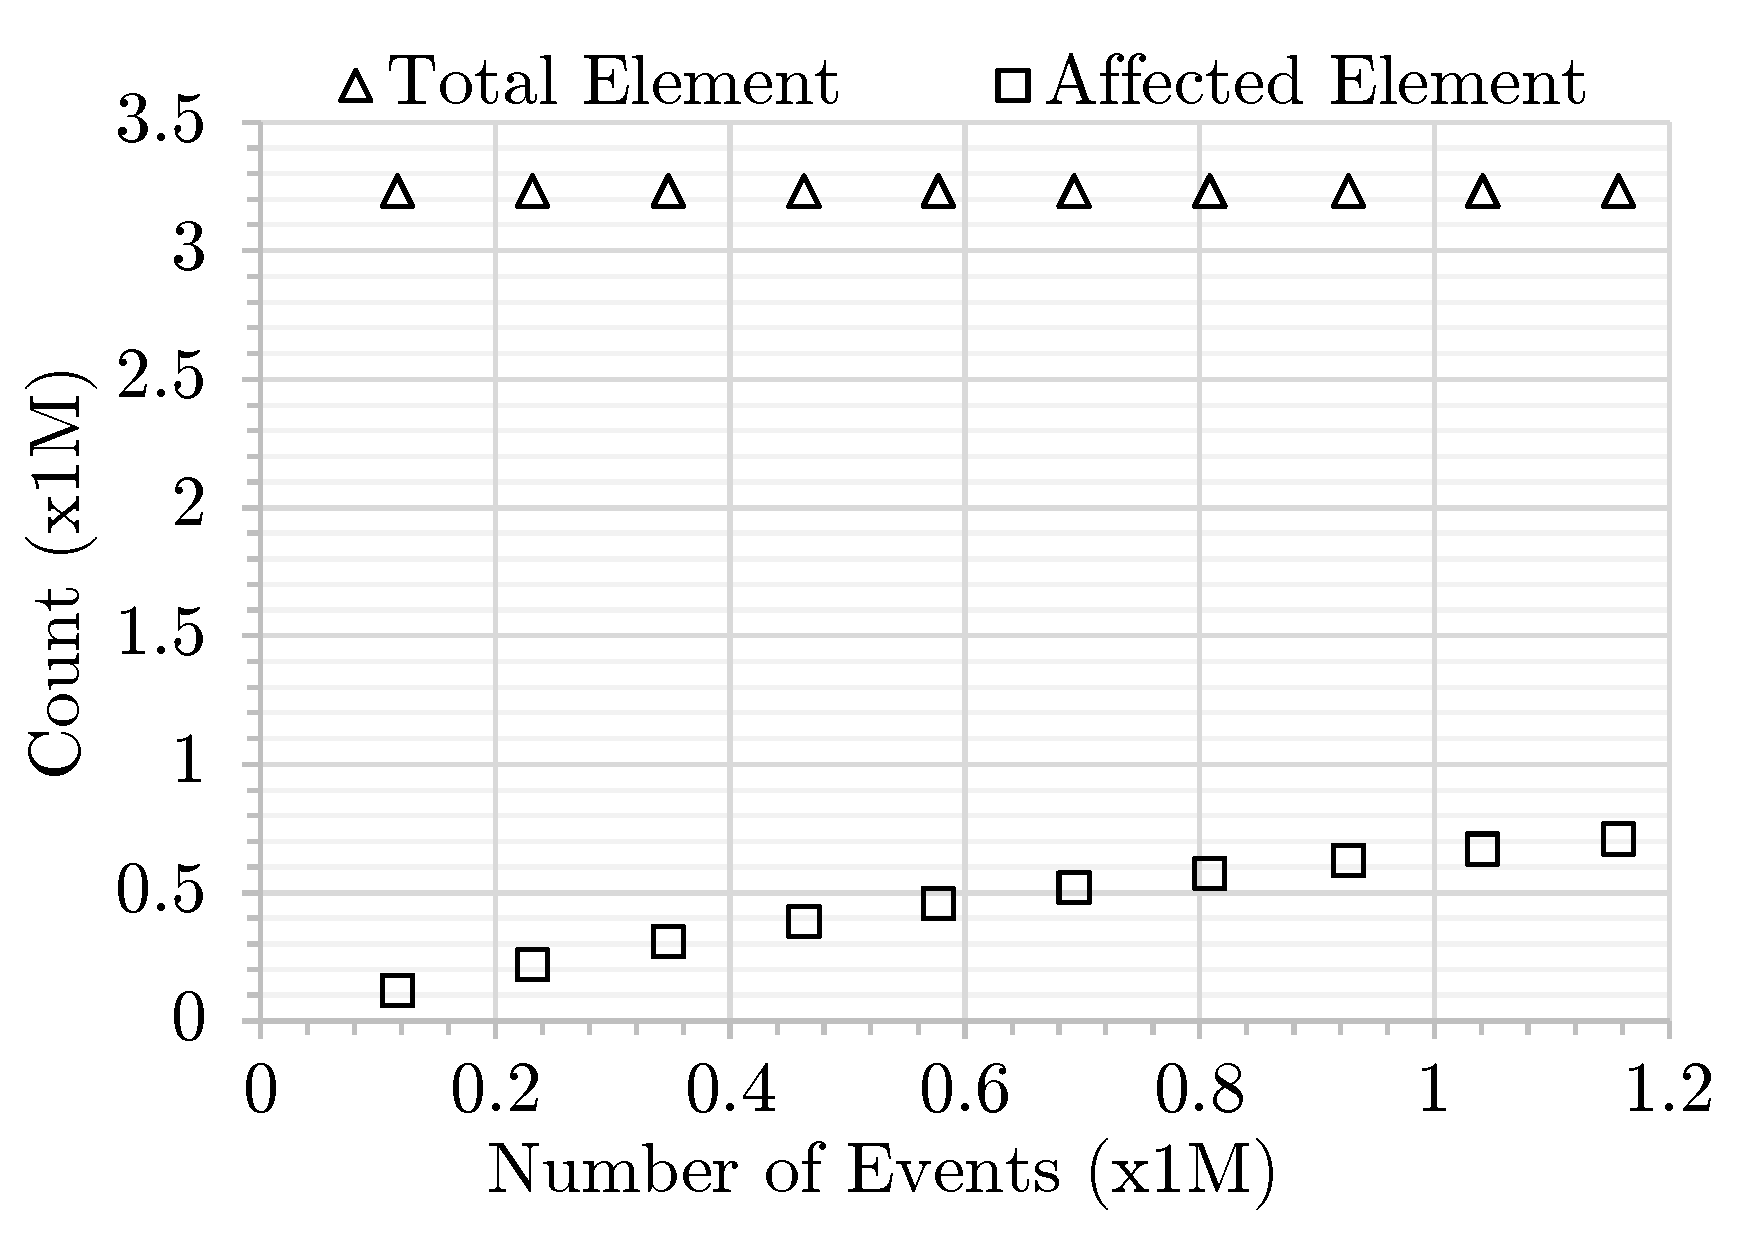
\includegraphics[width=\linewidth]{conflict-size-events}
	\caption{number of elements}
	\label{fig:conflict-size-events}
\end{subfigure}
\hfill
\begin{subfigure}[t]{0.490\linewidth}
	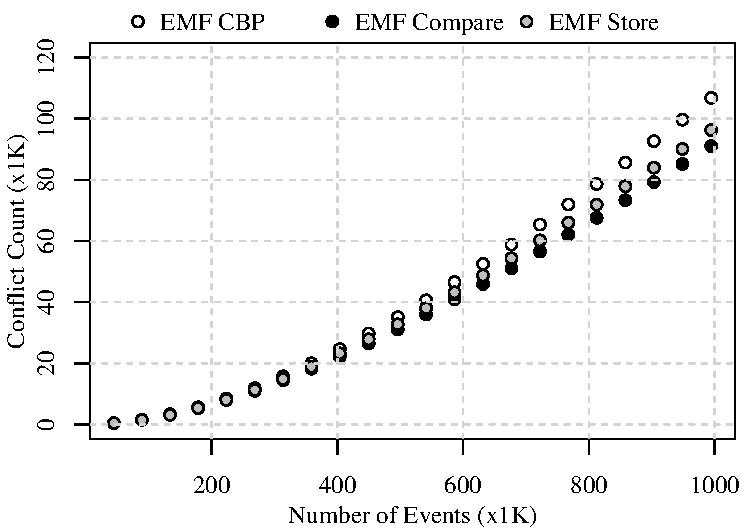
\includegraphics[width=\linewidth]{conflict-count-events}
	\caption{number of conflicts}
	\label{fig:conflict-count-events}
\end{subfigure}
\\
\begin{subfigure}[t]{0.490\linewidth}
	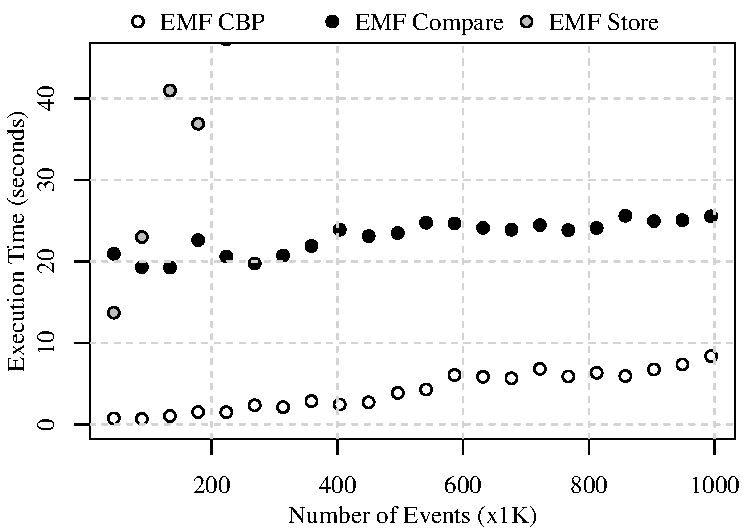
\includegraphics[width=\linewidth]{conflict-time-events}
	\caption{execution time}
	\label{fig:conflict-time-events}
\end{subfigure}
\hfill
\begin{subfigure}[t]{0.490\linewidth}
	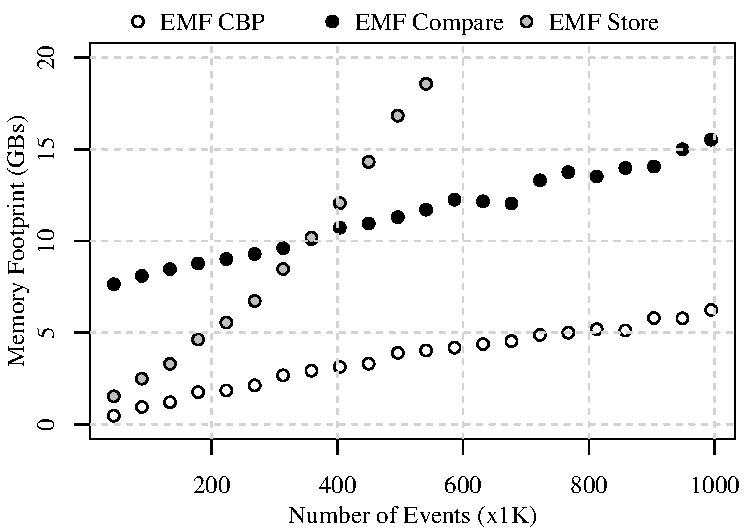
\includegraphics[width=\linewidth]{conflict-memory-events}
	\caption{memory footprint}
	\label{fig:conflict-memory-events}
\end{subfigure}
\caption{EMF CBP vs. EMF Compare vs. EMF Store comparison as change events increase.}
\label{fig:conflict_events}
\end{figure*}

Figure \ref{fig:conflict-time-events} exhibits EMF CBP outperforms EMF Compare and EMF Store in terms of execution time in detecting conflicts, even when the number of change events approaching a million. EMF Store is the slowest. It takes more than 35 seconds, even though the number of change events has just reached 0.1 million. Figure \ref{fig:conflict-memory-events} also shows EMF CBP outperforms EMF Compare and EMF Store in terms of memory footprint in conflict detection. At the last measurement point, a million change events, EMF CBP only consumes 6 GBs which is much less than EMF Compare and EMF Store. EMF Compare occupies around 16 GBs, while EMF Store already consumes the same amount of memory footprint only for 0.5 million change events.

\begin{figure*}[]
\centering
\begin{minipage}[b]{0.490\textwidth}
	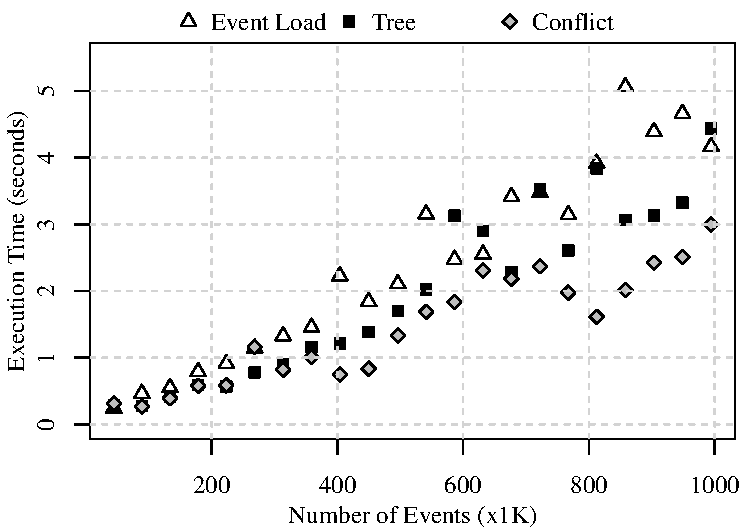
\includegraphics[width=\linewidth]{ecbp-conflict-time-events}
	\caption{A breakdown view of EMF CBP on the time required for conflict detection.}
	\label{fig:ecbp-conflict-time-events}    
\end{minipage}
\hfill
\begin{minipage}[b]{0.490\textwidth}
	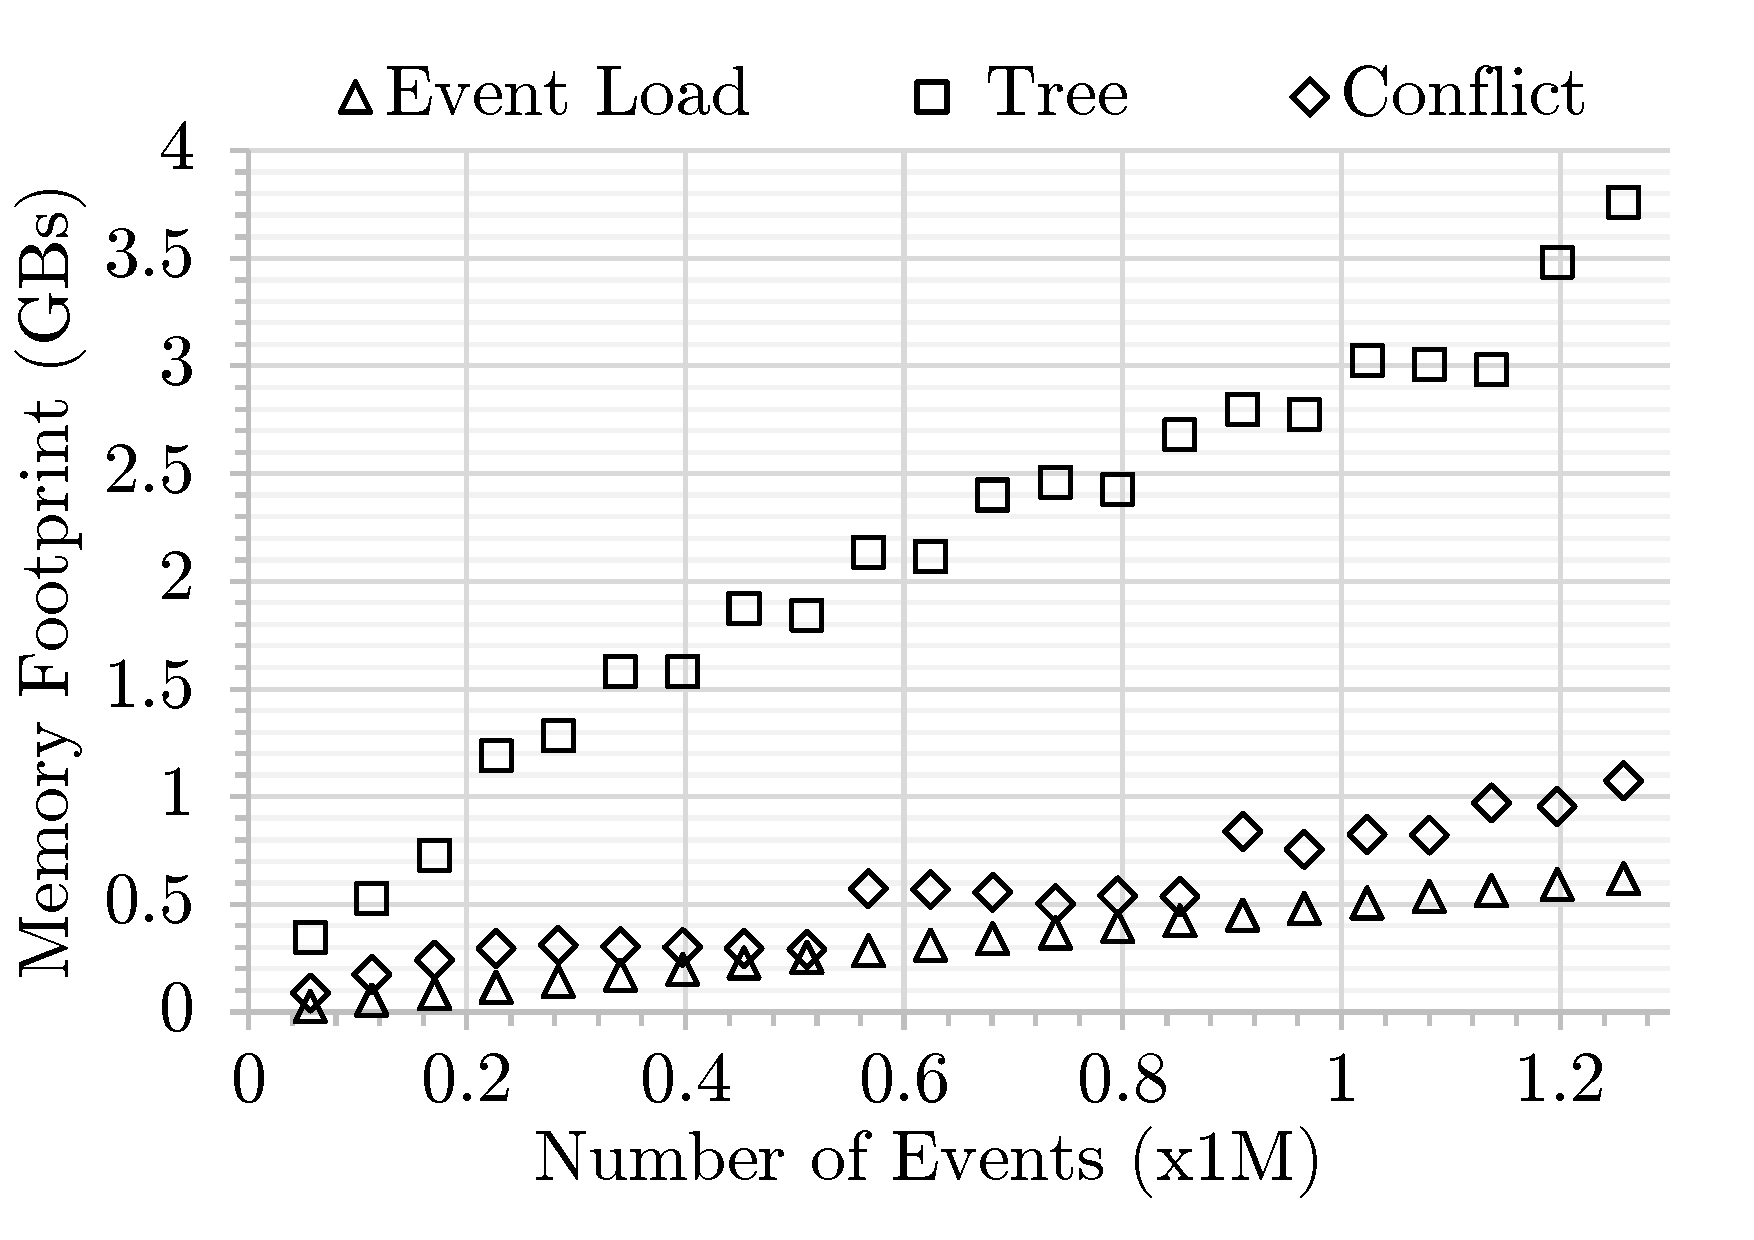
\includegraphics[width=\linewidth]{ecbp-conflict-memory-events}
	\caption{A breakdown view of EMF CBP on the memory footprint for conflict detection.}
	\label{fig:ecbp-conflict-memory-events}    
\end{minipage}  
\end{figure*}

\begin{figure*}[]
\centering
\begin{minipage}[b]{0.490\textwidth}
	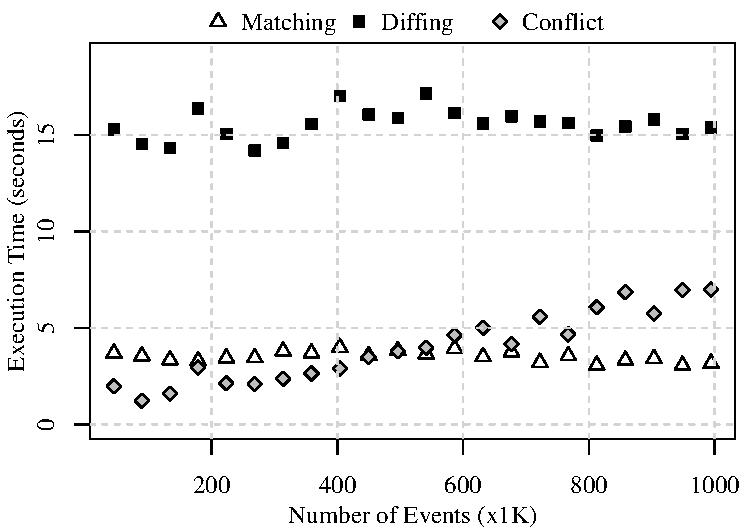
\includegraphics[width=\linewidth]{emfc-conflict-time-events}
	\caption{A breakdown view of EMF Compare on the time required for conflict detection.}
	\label{fig:emfc-conflict-time-events}
\end{minipage}
\hfill
\begin{minipage}[b]{0.490\textwidth}
	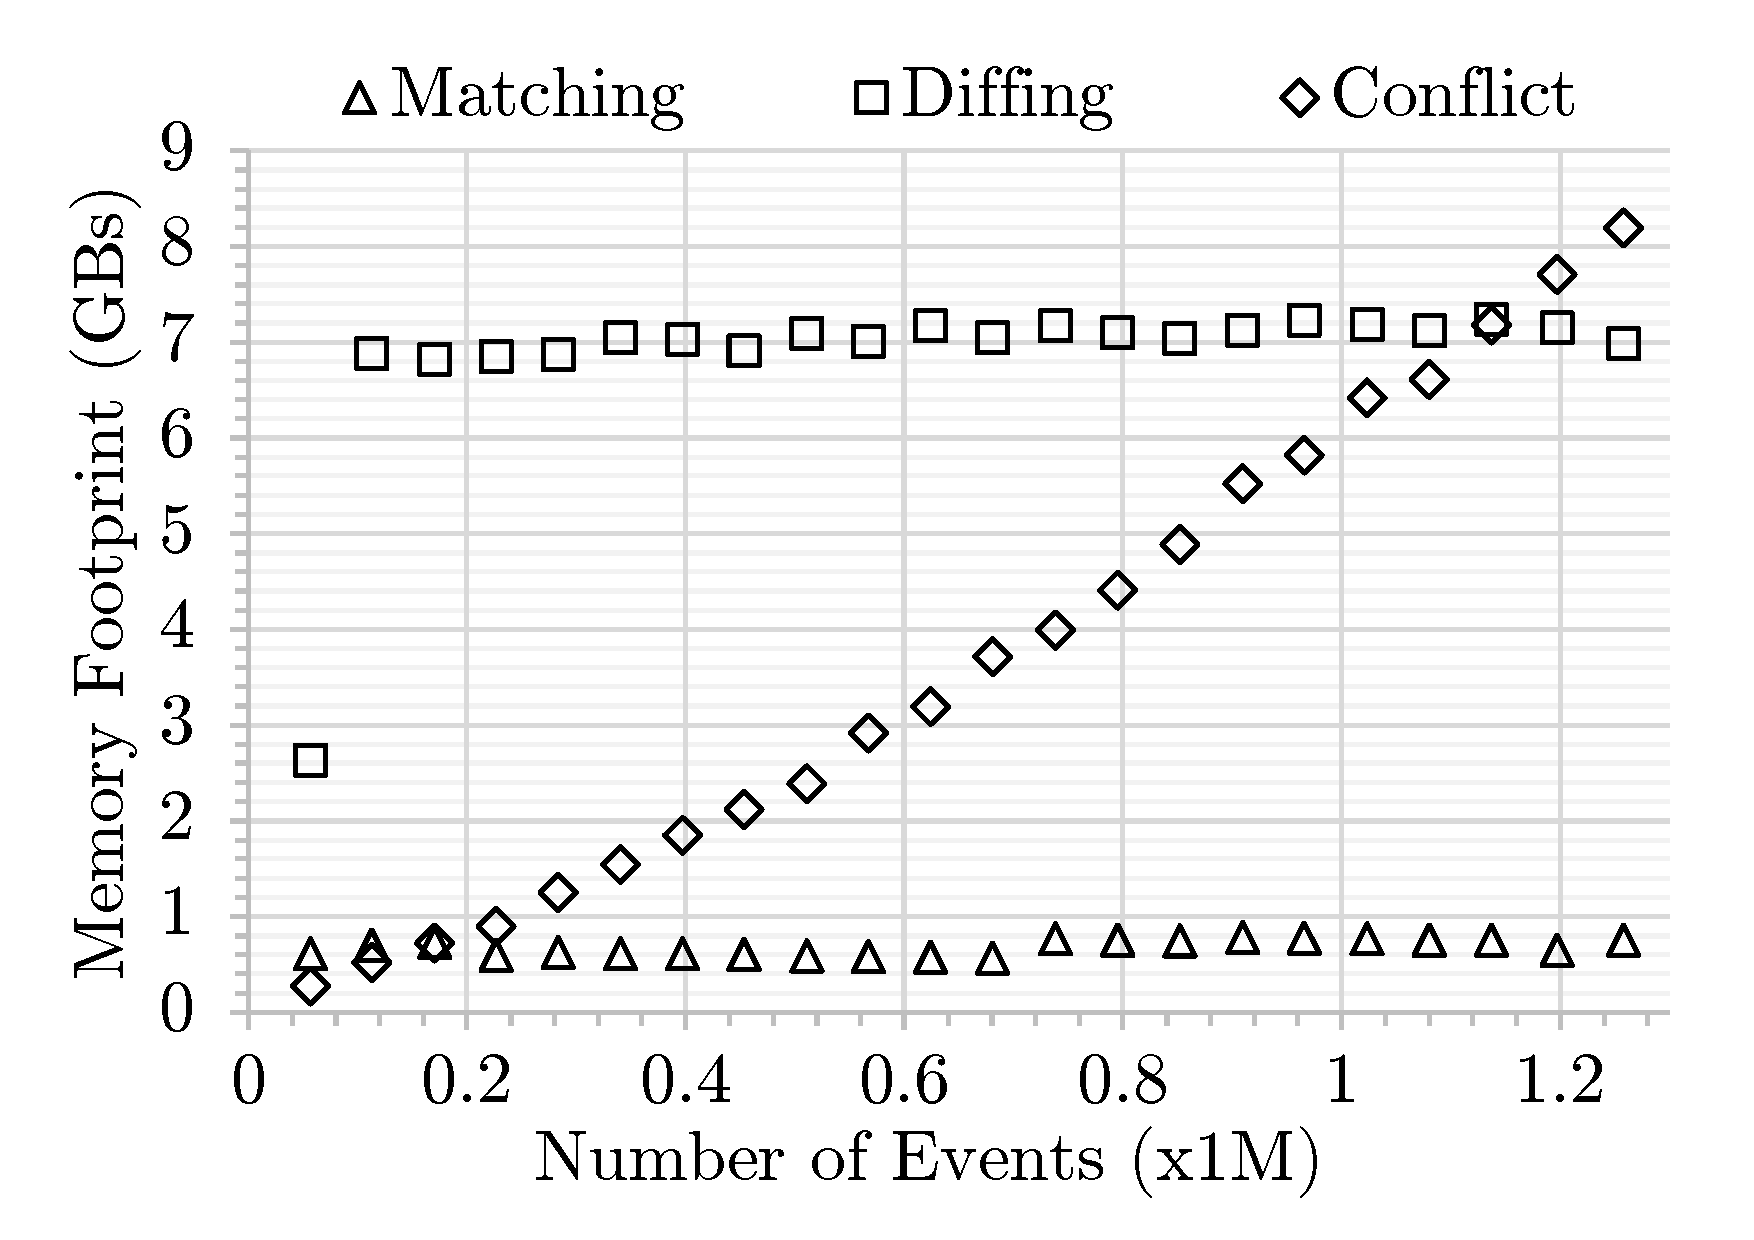
\includegraphics[width=\linewidth]{emfc-conflict-memory-events}
	\caption{A breakdown view of EMF Compare on the memory footprint for conflict detection.}
	\label{fig:emfc-conflict-memory-events}
\end{minipage}
\end{figure*}

\begin{figure*}[]
\begin{minipage}[b]{0.490\textwidth}
	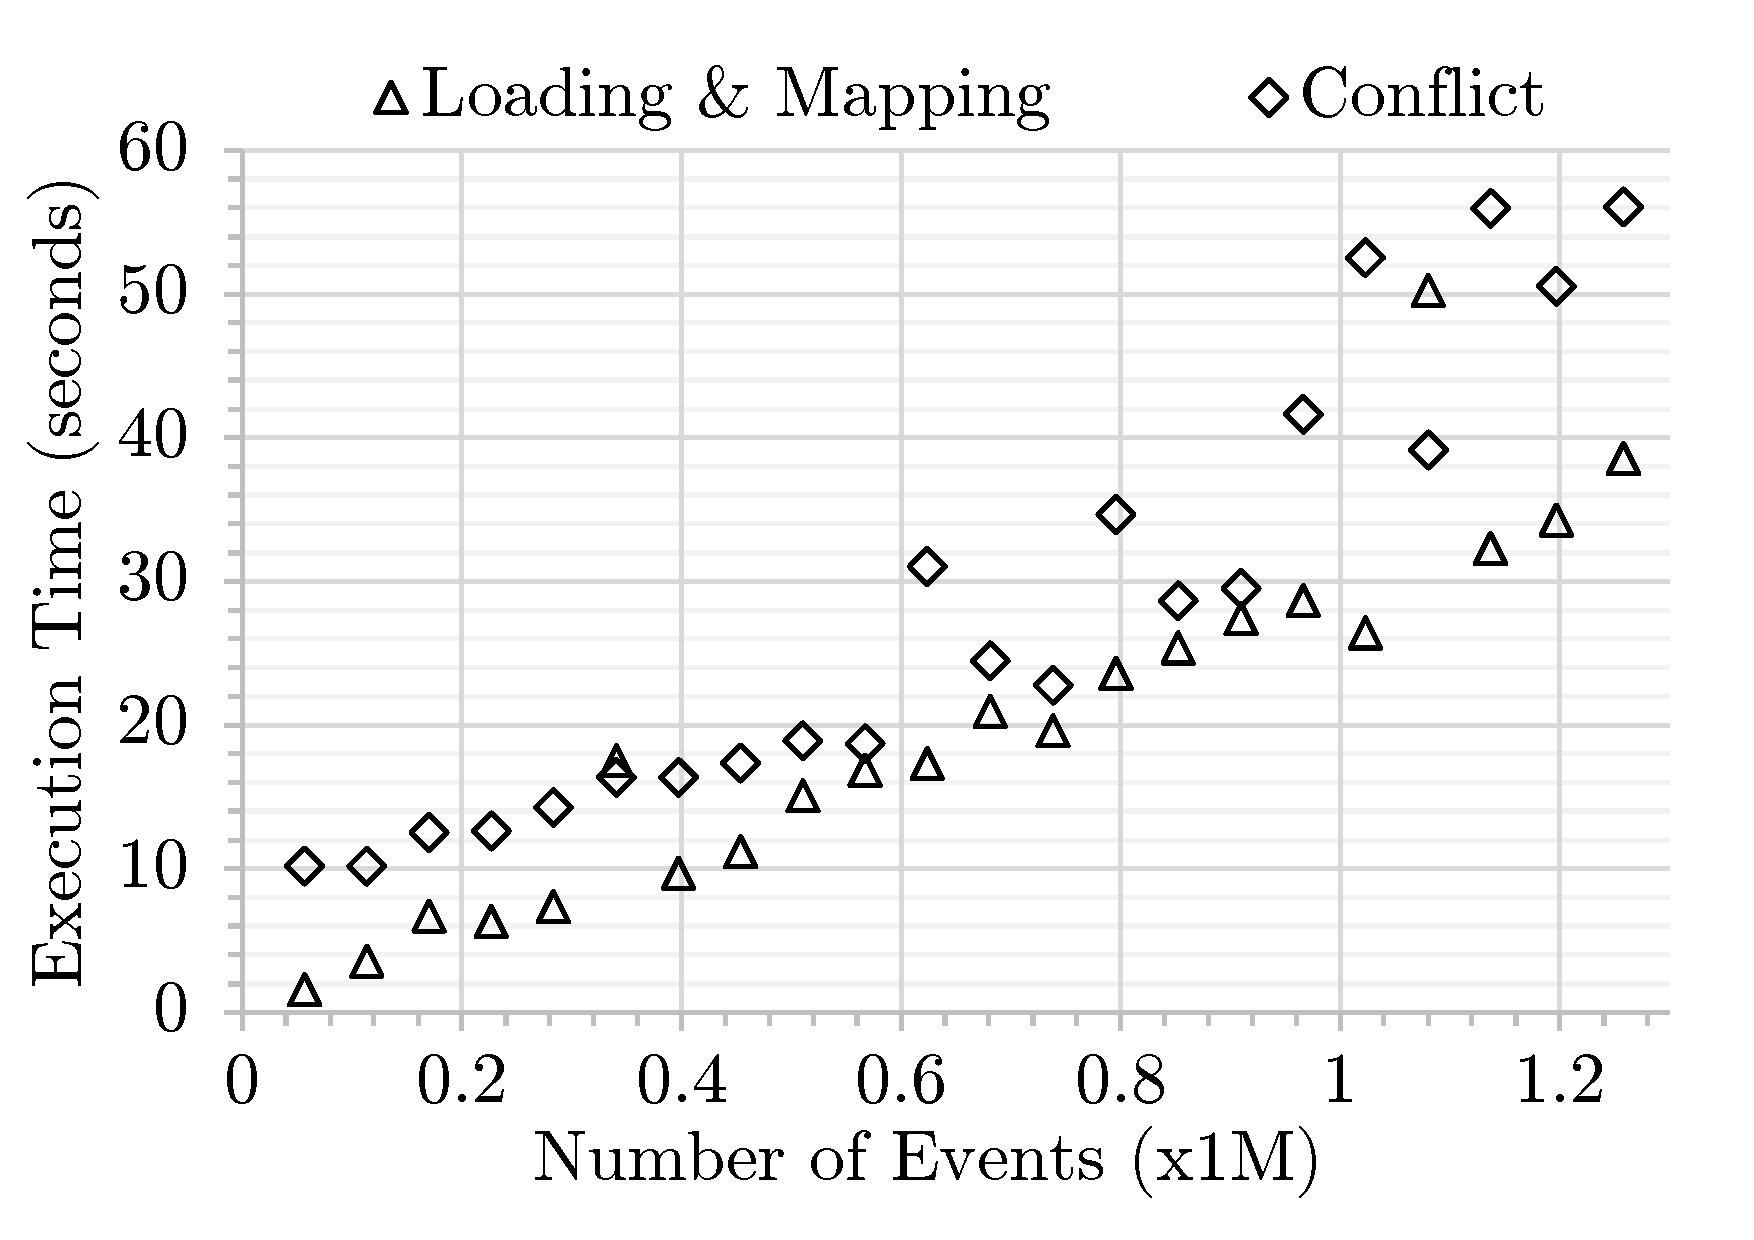
\includegraphics[width=\linewidth]{emfs-conflict-time-events}
	\caption{A breakdown view of EMF Store on the time required for conflict detection.}
	\label{fig:emfs-conflict-time-events}
\end{minipage}
\hfill
\begin{minipage}[b]{0.490\textwidth}
	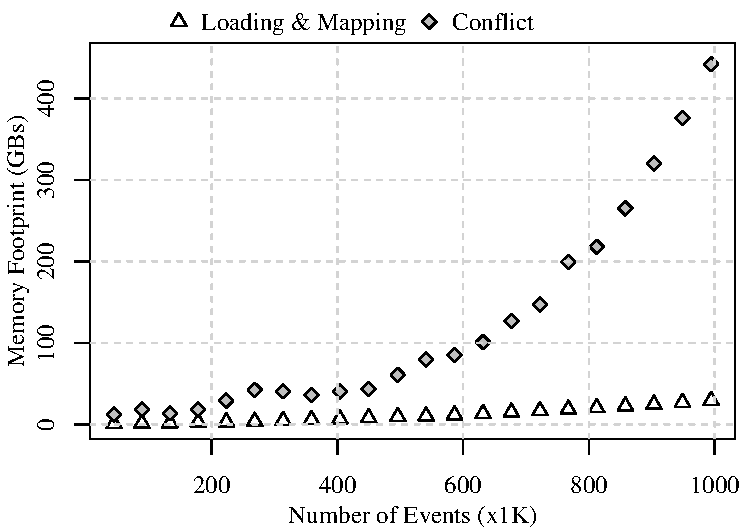
\includegraphics[width=\linewidth]{emfs-conflict-memory-events}
	\caption{A breakdown view of EMF Store on the memory footprint for conflict detection.}
	\label{fig:emfs-conflict-memory-events}
\end{minipage}
\end{figure*}

Figures \ref{fig:ecbp-conflict-time-events}, \ref{fig:emfc-conflict-time-events}, and \ref{fig:emfs-conflict-time-events} show the detailed view of EMF CBP, EMF Compare, and EMF Store on the time required to complete conflict detection. As can be seen in Figure \ref{fig:ecbp-conflict-time-events}, the time for EMF CBP to load change events, construct the element tree, and detect conflicts grows linearly. In detecting conflicts, the EMF CBP does not require differencing since changes are already available in the form of change events. Thus, differencing is not included in the diagram. 

In EMF Compare (Figure \ref{fig:emfc-conflict-time-events}), we can notice that the time taken for matching is less than 5 seconds, and the time used for identifying differences is around 15 seconds on average. The differencing takes a significant portion of the time since it needs to derive differences twice; differences between left and original models and right and original models. The time for matching and differencing tends to be constant since the sizes of the models are set to be as constant as possible (Figure \ref{fig:conflict-size-events}). In contrast, the time for detecting conflicts tends to grow due to the increasing number of conflicting changes as the number of change events increases. In detecting conflicts, EMF Store allocates most of the consumed time for identifying conflicts, and the time increases exponentially. The rest of the time is used for loading changes and mapping them to their affected elements and features (Figure \ref{fig:emfs-conflict-time-events}). 

In terms of memory footprint, EMF CBP allocates most of the memory space for element tree construction, and the rest is for the loading change events and identifying conflicts (Figure \ref{fig:ecbp-conflict-memory-events}). The reason for this is due to our technical implementation in constructing \textsf{elementTree}. A Feature can have many instances even though they refer to the same feature. This causes the memory to increase. One solution is to construct a partial metamodel so that a feature can only have one instance, and the instance is used as a key to access the feature's values in each element, similar to the implementation of the feature in EMF Framework. In EMF Compare (Figure \ref{fig:emfc-conflict-memory-events})), the amount of memory used for matching and differencing only increases slightly due to the sizes of the models that are set to be as constant as possible (Figure \ref{fig:conflict-size-events}). In contrast, the memory used for detecting conflict increases as the number of detected conflicts rises (Figure \ref{fig:conflict-count-events}). For EMF Store, the amount of memory used for loading changes and mapping increases slightly while the amount of memory for identifying conflicts grows exponentially (Figure \ref{fig:emfs-conflict-memory-events}).

\begin{figure*}[ht]
\centering
\begin{subfigure}[t]{0.490\linewidth}
	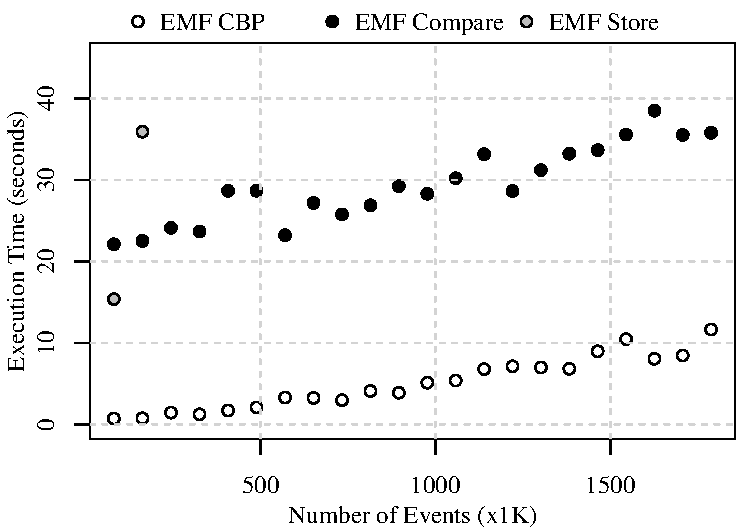
\includegraphics[width=\linewidth]{add-conflict-time-events}
	\caption{add-only}
	\label{fig:add-conflict-time-events}
\end{subfigure}
\hfill
\begin{subfigure}[t]{0.490\linewidth}
	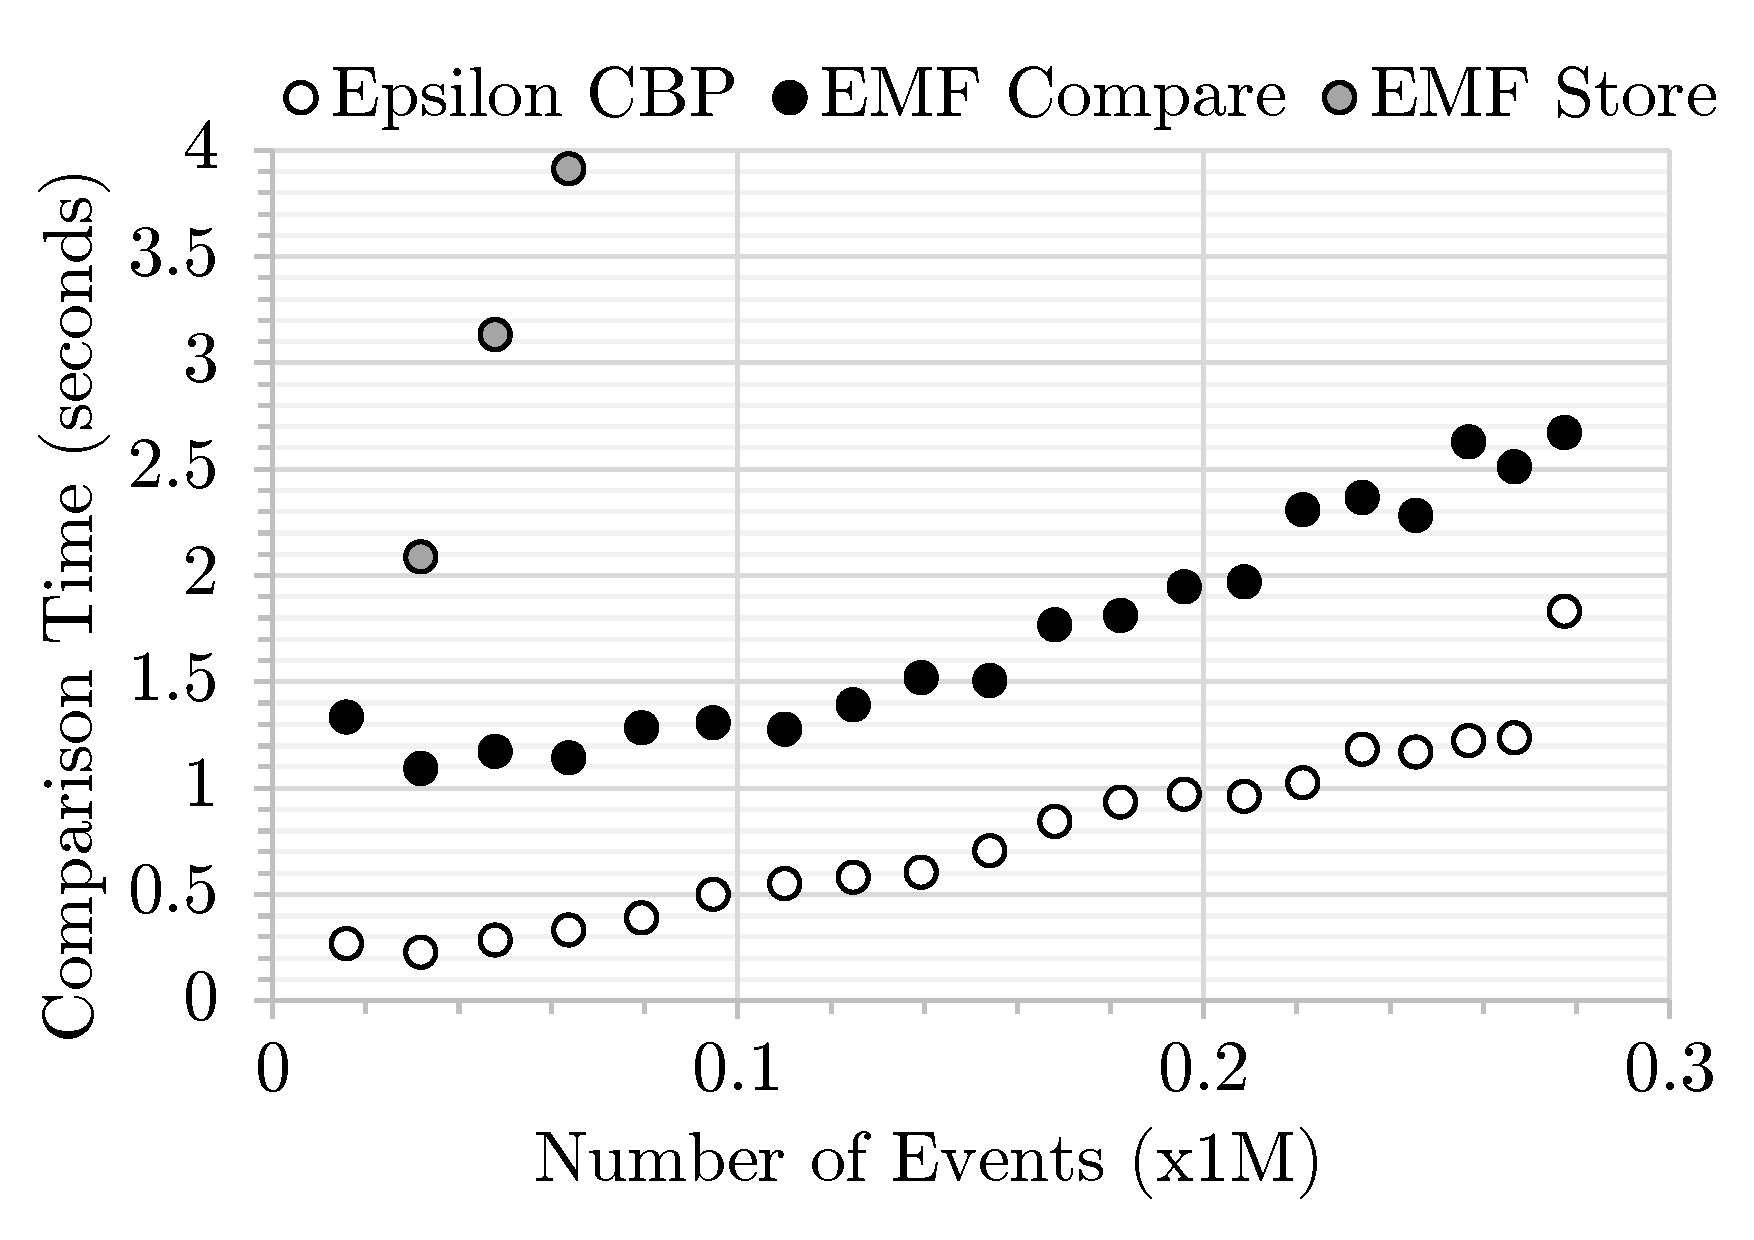
\includegraphics[width=\linewidth]{delete-conflict-time-events}
	\caption{delete-only}
	\label{fig:delete-conflict-time-events}
\end{subfigure}
\\
\begin{subfigure}[t]{0.490\linewidth}
	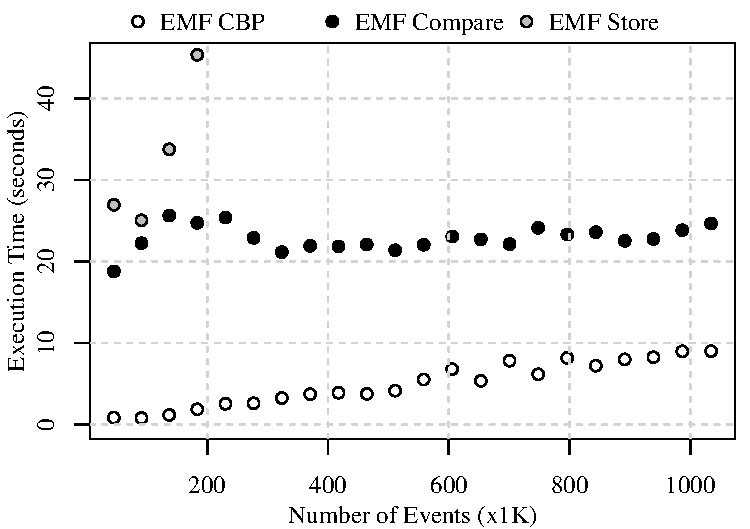
\includegraphics[width=\linewidth]{move-conflict-time-events}
	\caption{move-only}
	\label{fig:move-conflict-time-events}
\end{subfigure}
\hfill
\begin{subfigure}[t]{0.490\linewidth}
	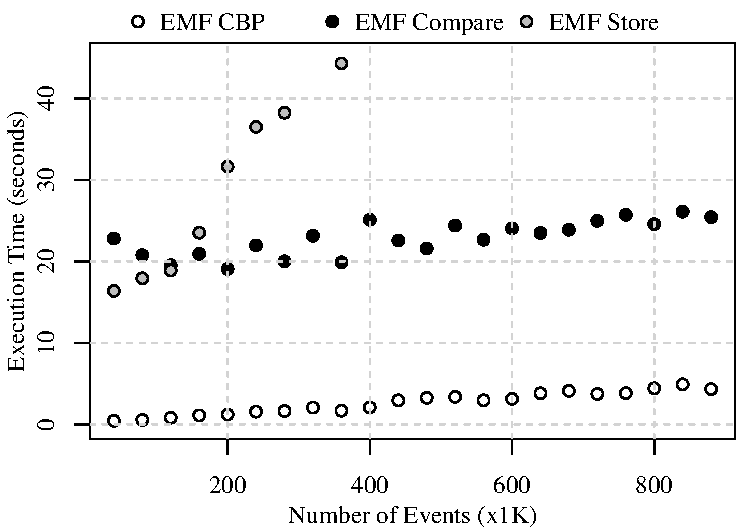
\includegraphics[width=\linewidth]{change-conflict-time-events}
	\caption{change-only}
	\label{fig:change-conflict-time-events}
\end{subfigure}
\caption{Conflict detection time for homogeneous operations.}
\label{fig:homgeneous_operation_time_events}
\end{figure*}

From the last measure point of the mixed-operation experiment, around 91 thousand conflicts were detected by EMF Compare, and about 3 thousand (3.3\%) of them cannot be detected by EMF CBP. This is due to the derived move changes produced by EMF Compare, which are different from the real changes recorded by EMF CBP. In contrast, EMF CBP detects around 107 thousand conflicts, and there are approximately 19 thousand (18\%) conflicts that EMF Compare cannot detect; the number consists of 6.6 thousand (6.6\%) actual move conflicts, 8.2  thousand (7.6\%) one-sided reset conflicts, and 4.1 thousand (3.8\%) single-valued containment conflicts (see Section \ref{sec:emf_cbp_vs_emf_compare} to find the definitions of these kinds of conflicts). Thus, 88 thousand (91 - 3 = 107 - 19 thousands) conflicts can be detected by both.

From 107 thousand conflicts detected by EMF CBP, there are 3.7 million (3.5\%) conflicts that cannot be detected by EMF Store, which is caused by the first-time move conflict (see Section \ref{sec:emf_cbp_vs_emf_store}). By contrast, EMF CBP cannot detect 1.8 thousands (1.8\%) of the 96.4 thousand conflicts detected by EMF Store due to the two-sided reset conflicts (see Section \ref{sec:emf_cbp_vs_emf_store}). 

%Total dirty conflicts = 4190
%Derived Moves = 3023
%Conflicts by deletion = 1167
%Other conflicts = 0
%Conflicts by non-deletion = 3023
%Real undentected conflicts = 3023
%EMF Compare conflicts: 91075


%DETAILS OF UNDETECTED CONFLICTS BY EMF COMPARE
%Total dirty conflicts = 20156
%Derived Moves = 6658
%Reset-to-original conflicts = 8271
%Conflicts by deletion = 1073
%Modify single-valued containment conflicts = 4154
%Other conflicts = 0
%Conflicts by non-deletion = 19083
%Real undentected conflicts = 19083
%CBP conflicts: 107058
%
%
%//--------------------------------------------emf cbp vs emf store
%Undetected CBP conflicts: 3734
%Modified position conflicts: 3722
%Other conflicts: 12
%All CBP conflicts: 107058
%
%Undetected EMFStore conflicts: 1823
%Move to original position conflicts: 852
%Set to original value conflicts: 961
%Other conflicts: 10
%All EMFStore conflicts: 96417

\subsection{Homogenous Operations}
\label{sec:homogenous-operation_conflict}

\subsubsection{Detection Time} 
\label{sec:detection_time}
Figure \ref{fig:homgeneous_operation_time_events} depicts the results of conflict detection time between EMF CBP, EMF Compare, and EMF Store in homogenous operations. The results show that EMF CBP is faster at detecting conflicts than EMF Compare and EMF Store in all types of homogenous operations. The latter has the worst performance in most cases except in the delete-only experiment. In this case, EMF Compare is the slowest. EMF Compare also requires calculating dependencies between conflicts. So, when the number of deletions is excessive, EMF Compare performs less efficiently than EMF Store (Figure \ref{fig:delete-conflict-time-events}). In the evaluation, this happens when the number of change events exceeds 240 thousand.

\subsubsection{Memory Footprint}
\label{sec:memory_footprint}
Figure \ref{fig:homgeneous_operation_memory_events} illustrates the memory footprint resulting from conflict detection in EMF CBP, EMF Compare, and EMF Store with homogeneous operations. The Figure displays that EMF CBP outperforms EMF Compare and EMF Store in terms of memory footprint. EMF CBP only performs worse than EMF Compare in the delete-only experiment when the number of change events is more than 80 thousand -- model size is 39.5 thousand elements each (Figure \ref{fig:delete-conflict-memory-events}). In terms of memory footprint, EMF Store performs worse than EMF CBP and EMF Compare. It only performs better than EMF Compare when the number of change events is relatively small -- less than 25 thousand change events. 

\begin{figure*}[ht]
\centering
\begin{subfigure}[t]{0.490\linewidth}
	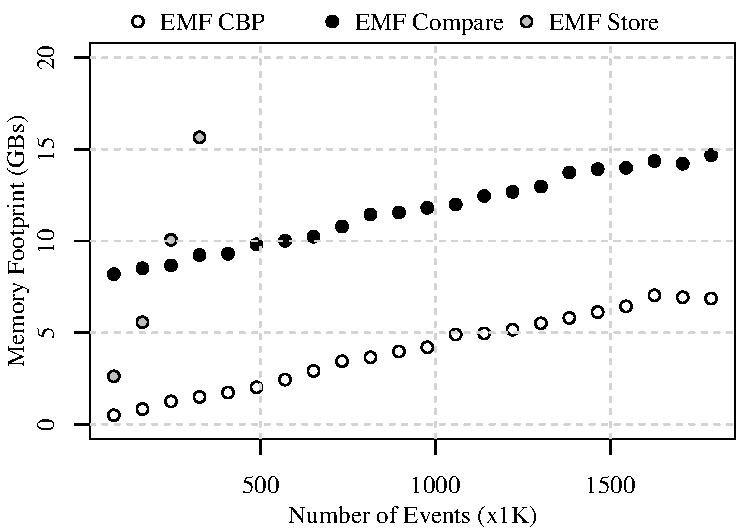
\includegraphics[width=\linewidth]{add-conflict-memory-events}
	\caption{add-only}
	\label{fig:add-conflict-memory-events}
\end{subfigure}
\hfill
\begin{subfigure}[t]{0.490\linewidth}
	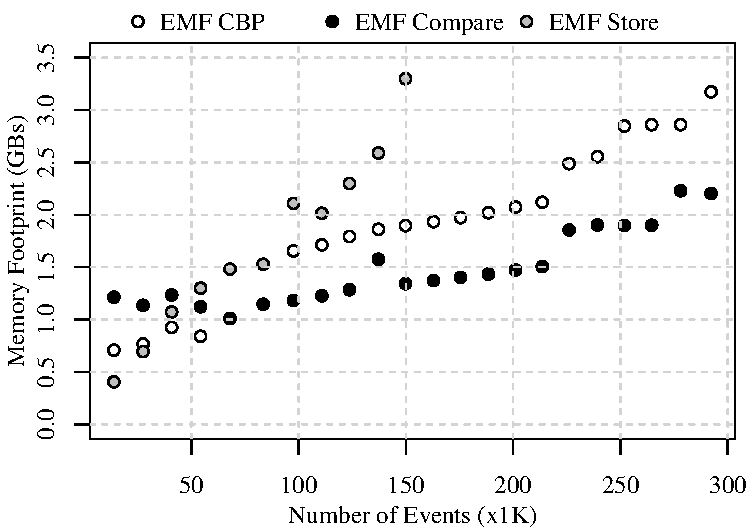
\includegraphics[width=\linewidth]{delete-conflict-memory-events}
	\caption{delete-only}
	\label{fig:delete-conflict-memory-events}
\end{subfigure}
\\
\begin{subfigure}[t]{0.490\linewidth}
	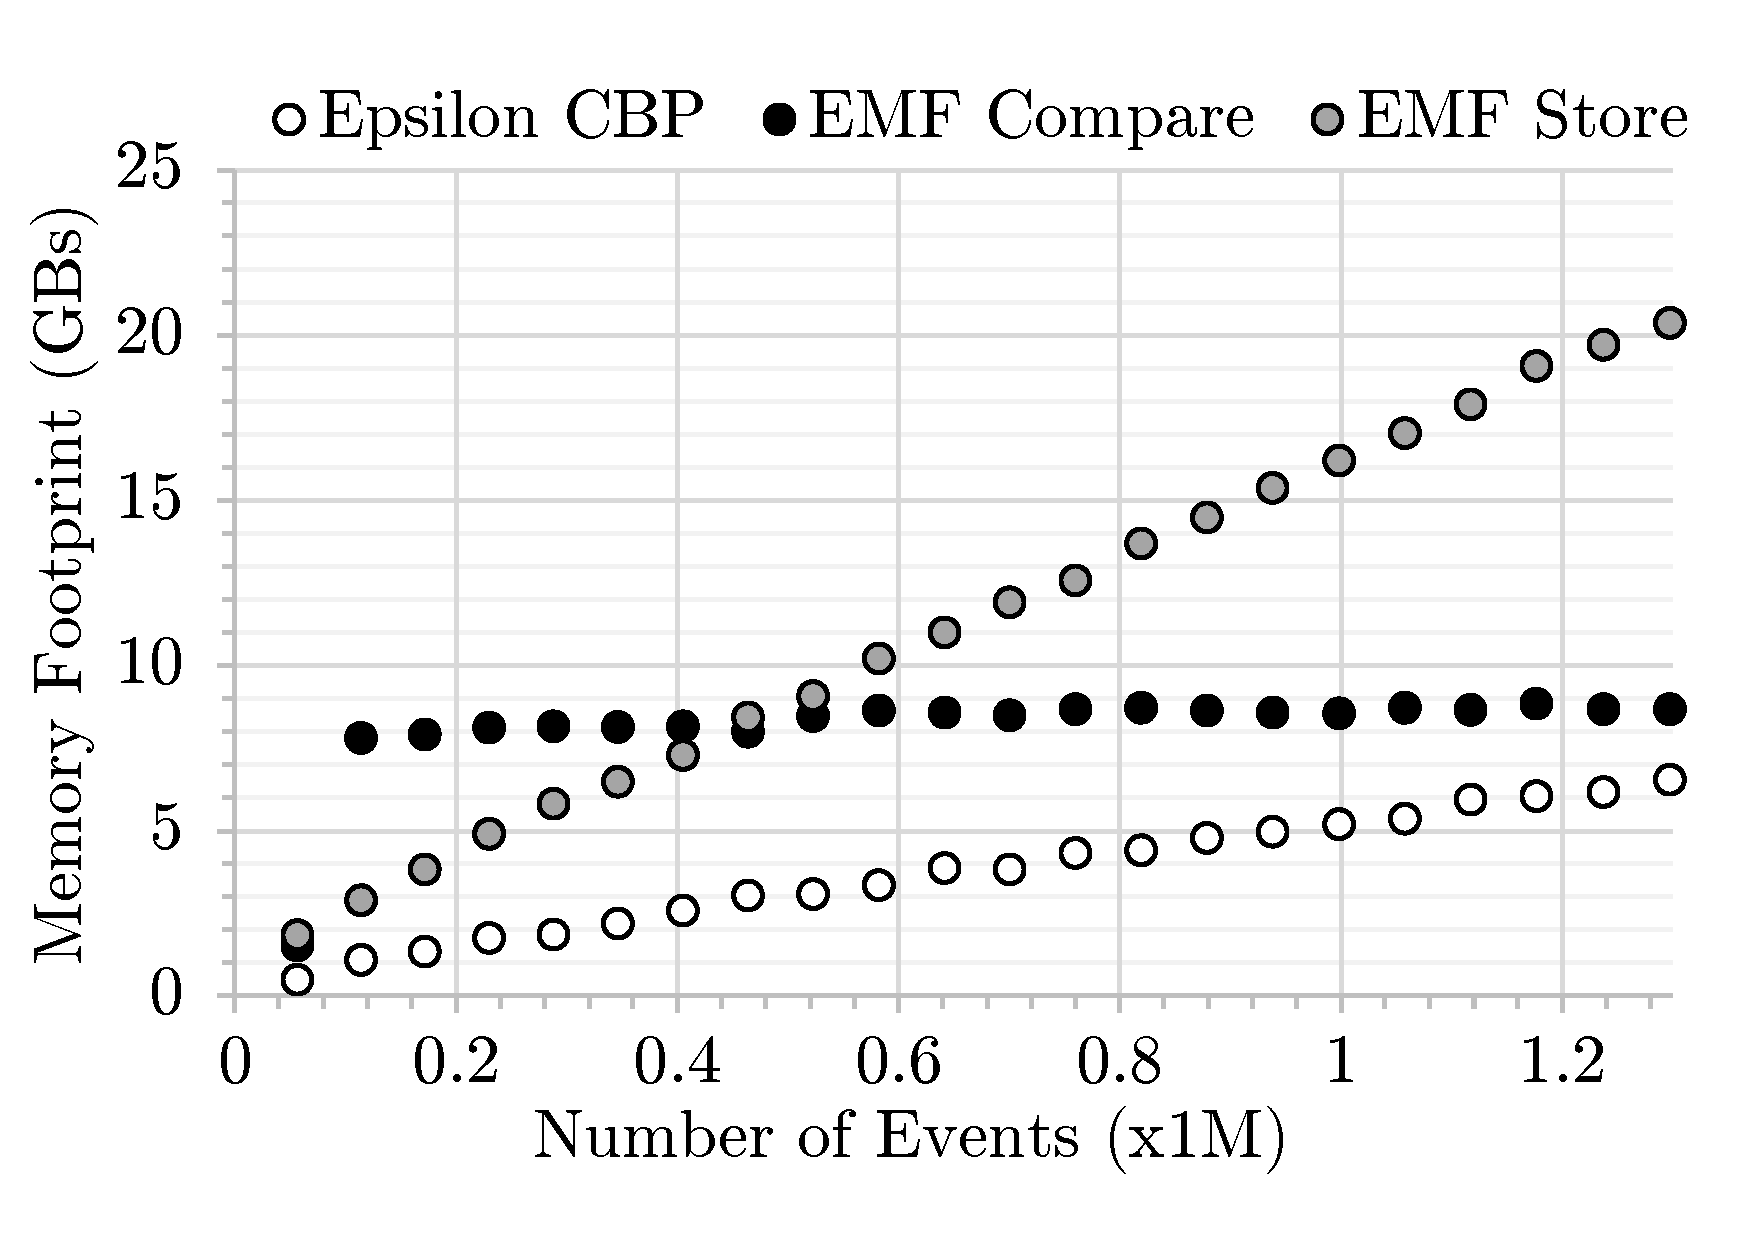
\includegraphics[width=\linewidth]{move-conflict-memory-events}
	\caption{move-only}
	\label{fig:move-conflict-memory-events}
\end{subfigure}
\hfill
\begin{subfigure}[t]{0.490\linewidth}
	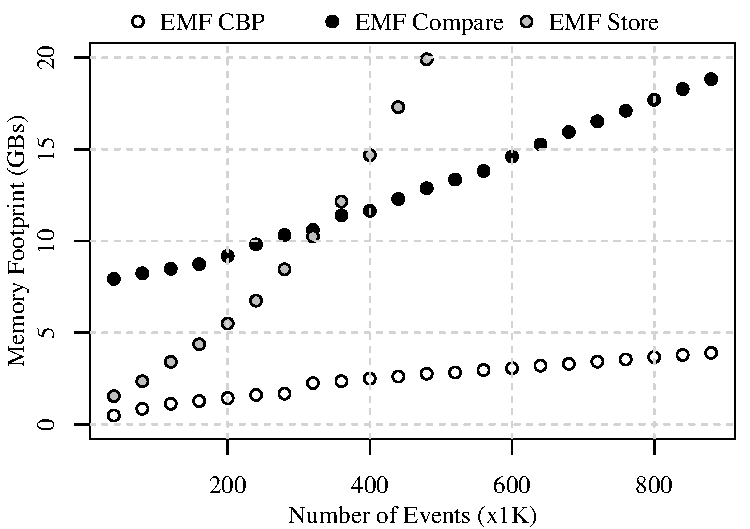
\includegraphics[width=\linewidth]{change-conflict-memory-events}
	\caption{change-only}
	\label{fig:change-conflict-memory-events}
\end{subfigure}
\caption{Conflict detection memory for homogeneous operations.}
\label{fig:homgeneous_operation_memory_events}
\end{figure*}

In Figure \ref{fig:move-conflict-memory-events}, EMF CBP's memory footprint tends to increase faster than EMF Compare's memory footprint. This is possible since the change events of EMF Compare are actually minimal differences that are derived from model differencing, which in terms of number is less than actual change events recorded in EMF CBP. Therefore, more random change events mean a higher possibility to produce more conflicts.

\subsubsection{Conflict Count}
\label{sec:conflict_count}
Figure \ref{fig:homgeneous_operation_count_events} displays the number of conflicts, both \textsf{REAL} and \textsf{PSEUDO}, detected by EMF CBP, EMF Compare, and EMF Store in the context of homogenous operations. In the add-only experiment as displayed in Figure \ref{fig:add-conflict-count-events}, all of them detect the same number of conflicts.

\begin{figure*}[ht]
\centering
\begin{subfigure}[t]{0.490\linewidth}
	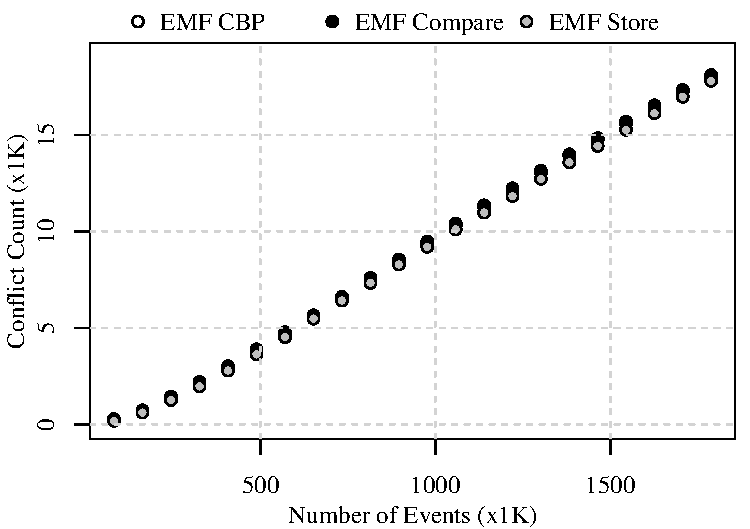
\includegraphics[width=\linewidth]{add-conflict-count-events}
	\caption{add-only}
	\label{fig:add-conflict-count-events}
\end{subfigure}
\hfill
\begin{subfigure}[t]{0.490\linewidth}
	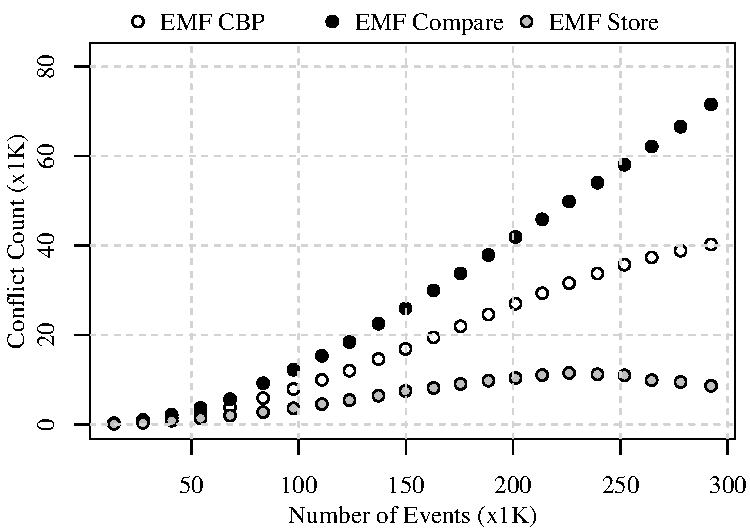
\includegraphics[width=\linewidth]{delete-conflict-count-events}
	\caption{delete-only}
	\label{fig:delete-conflict-count-events}
\end{subfigure}
\\
\begin{subfigure}[t]{0.490\linewidth}
	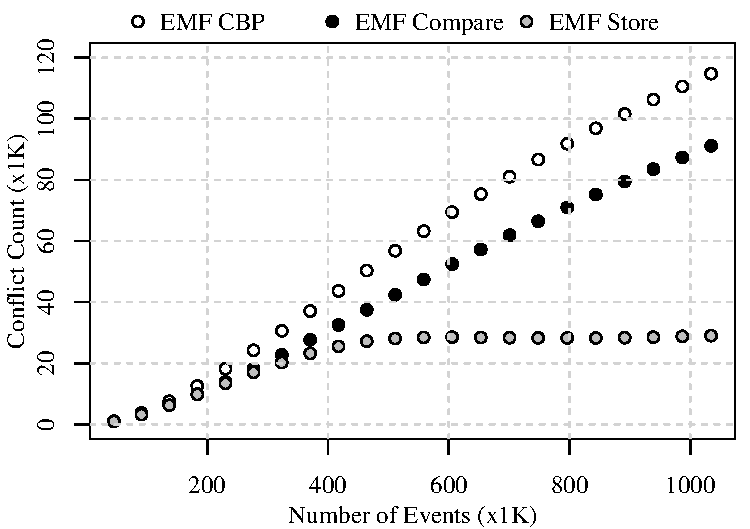
\includegraphics[width=\linewidth]{move-conflict-count-events}
	\caption{move-only}
	\label{fig:move-conflict-count-events}
\end{subfigure}
\hfill
\begin{subfigure}[t]{0.490\linewidth}
	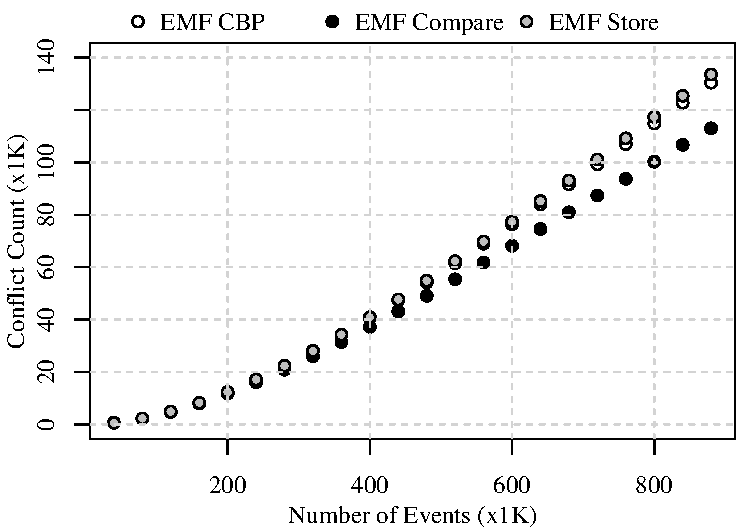
\includegraphics[width=\linewidth]{change-conflict-count-events}
	\caption{change-only}
	\label{fig:change-conflict-count-events}
\end{subfigure}
\caption{Conflict detection count for homogeneous operations.}
\label{fig:homgeneous_operation_count_events}
\end{figure*}

Figure \ref{fig:change-conflict-count-events} shows the results of the change-only experiment. We can notice that the number of conflicts detected by EMF Compare is lower than EMF CBP. This is mainly because EMF Compare detects no change on an element or feature that has been modified but finally changed back to its original state. While in EMF CBP, this is counted as a change with potential to raise a {PSEUDO} conflict as defined and showed in (\ref{eq:ecbp_pseudoconflict}), Section \ref{sec:emf_cbp_vs_emf_compare}, and Figure \ref{fig:statechart_04}. At the last measurement point in Figure \ref{fig:change-conflict-count-events}, there are 17 thousand (13.1\% of 130 thousand EMF CBP conflicts) of this kind of conflict undetected by EMF Compare. EMF Compare itself only detects 113 thousand conflicts. 

It can also be noticed that the number of conflicts detected by EMF CBP is slightly less than EMF Store detects. This happens because, as previously discussed, EMF Store does not consider states in detecting conflicts thus, two different change events that are applied to the same element or feature, even though they yield eventual states that are equal to their original state are considered in conflict. In Figure \ref{fig:change-conflict-count-events}, at the last measurement point, in total, EMF Store detects 133 thousand conflicts but 3.1 thousands (2.3\%) of them cannot be detected by EMF CBP due to this two-sided reset conflict (see Section \ref{sec:emf_cbp_vs_emf_store}). 

In the delete-only experiment in Figure \ref{fig:delete-conflict-count-events}, EMF CBP and EMF Compare detect more conflicts than EMF Store since they do not put a conflict that depends on another conflict into one group as performed by EMF Store as has been discussed in Section \ref{sec:emf_cbp_vs_emf_store}. As the number of change events grows, the number of conflicts that share the same change events also increases. Thus, these conflicts are grouped into one conflict causing the number of conflicts decreasing (see Section \ref{sec:emf_cbp_vs_emf_store}). In addition, EMF CBP detects fewer conflicts than EMF Compare since it skips calculating conflicts for features and values of an element that have been deleted. Change events that affect the features and values have been included when calculating conflicts caused by the deletion of the element, as been explained in the last paragraph of Section \ref{sec:delete_conflict}. In contrast, EMF Compare treats the conflicts at the features and values of a deleted element as separate conflicts. 

%DETAILS OF UNDETECTED CONFLICTS BY CBP
%Total dirty conflicts = 44062
%Derived Moves = 0
%Conflicts by deletion = 44062
%Other conflicts = 0
%Conflicts by non-deletion = 0
%Real undentected conflicts = 0
%EMF Compare conflicts: 73610
%
%
%DETAILS OF UNDETECTED CONFLICTS BY EMF COMPARE
%Total dirty conflicts = 5615
%Derived Moves = 0
%Reset-to-original conflicts = 0
%Conflicts by deletion = 5615
%Modify single-valued containment conflicts = 0
%Other conflicts = 0
%Conflicts by non-deletion = 0
%Real undentected conflicts = 0
%CBP conflicts: 37333
%
%----
%
%UNDETECTED CONFLICTS BY EMFSTORE:
%Undetected CBP conflicts: 0
%Modified position conflicts: 0
%Other conflicts: 0
%All CBP conflicts: 37333
%
%UNDETECTED CONFLICTS BY CBP:
%Undetected EMFStore conflicts: 0
%Move to original position conflicts: 0
%Set to original value conflicts: 0
%Other conflicts: 0
%All EMFStore conflicts: 8392


Figure \ref{fig:move-conflict-count-events} shows the results of the move-only experiment. EMF CBP detects more conflicts than EMF Compare since it has more change events than EMF Compare due to the use of actual records of changes. In EMF Compare, its change events are derived and effective, which means the minimum number of change events are produced. Less number of change events means less probable to produce conflicts. EMF Store detects fewer conflicts than EMF CBP and EMF Compare due to grouping of conflicts that depend on each other as has discussed in Section \ref{sec:emf_cbp_vs_emf_store}.

Using the data of conflicts from the last measurement point in Figure \ref{fig:move-conflict-count-events}, we identify that, from 91.6 thousand conflicts detected by EMF Compare, 4.7 thousand (5.1\%) of them are derived move conflicts which EMF CBP cannot detect. By contrast, from 114.8 thousand conflicts detected by EMF CBP, there are 27.9 million (24.3\%) conflicts cannot be detected by EMF Compare, consisting of 20.3 thousand (17.7\%) real move conflicts and 7.6 thousand (6.6\%) single-valued containment conflicts (see Section \ref{sec:emf_cbp_vs_emf_compare}). We also identify that, from 115 thousand conflicts detected by EMF CBP, 17 thousand (14.8\%) of them are undetected by EMF Store due to the first-time move conflict explained in Section \ref{sec:emf_cbp_vs_emf_store}. On the other hand, from all 29.5 thousand conflicts detected by EMF Store, only 2.5 thousand (8.5\%) of them cannot be detected by EMF CBP due to the two-sided reset conflict presented in Section \ref{sec:emf_cbp_vs_emf_store}.

\subsection{Limitations and Validity}
\label{sec:limitation_and_Threat_to_validity}
We have only tested the proposed algorithms on synthetic models, which were reversed engineered from a single real-world software project, Epsilon \cite{eclipse2018epsilongit}. Therefore, the generated models may not represent the complexity and interconnectedness of models in other domains. Diverse characteristics of models in different domains can affect the algorithm's effectiveness and therefore yield different outcomes. Moreover, the generated models from the reverse engineering are limited to Modisco Java \cite{eclipse2018modiscojava} metamodel only. Thus, there is no guarantee that it will perform consistently on models conforming to different metamodels.

For the proposed conflict detection solution, we have tried to cover as much as common changes made in EMF models (e.g. performing \textsf{add}/\textsf{remove}/\textsf{set}/\textsf{move} operations on \textsf{single}/\textsf{multi}-\textsf{valued} features, \textsf{attribute}/\textsf{reference} features, or \textsf{containment}/\textsf{non}-\textsf{containment} references), the random modification made in the evaluation does not largely reflect the evolution of models in the real world. This is challenging as different domains can have their own patterns of model evolution -- different problems, metamodels, modellers, etc. So far, the most complex composite changes applied to the random modification are limited to \textsf{move} and \textsf{delete} changes only (\textsf{move} event consists of \textsf{remove} and \textsf{add} events, while \textsf{delete} event also removes the sub-elements of the deleted element). More complex composite changes, such as refactoring, have not been evaluated. Also, the random modification does not consider the correctness of the changes since it might break certain constraints of the models. For example, in Java \cite{eclipse2018modiscojava} models, removing a parameter from a function causes errors in the function's body but are ignored in the evaluation. 

\section{Related Work}
\label{sec:related_work}
By default, modelling tools that support the 3-layer metamodelling architectures of Eclipse Modelling Framework (EMF) \cite{steinberg2008emf} employ state-based persistence to persist models in Metadata Interchange (XMI) format. XMI is a standard issued by Object Management Group (OMG) for exchanging metadata information via Extensible Markup Language (XML) \cite{omg2018xmi}. There are several non-XMI approaches to state-based model persistence that use relational or NoSQL databases. For example, EMF Teneo \cite{eclipse2017teneo} persists EMF models in relational databases, while Morsa \cite{DBLP:conf/models/Espinazo-PaganCM11} persist models in documents with MongoDB backend \cite{mongodb}, and NeoEMF \cite{daniel2016neoemf} persists models in while NeoEMF persists models in multi-NoSQL backends: Neo4j \cite{neo4j2019neo4j} for Graph, MapDB \cite{mapdb2019mapdb} for Map, and Apache HBase \cite{apache2019hbase} for Column datastores. However, none of these approaches provides built-in support for versioning and models are eventually stored in binary files/folders, which are known to be a poor fit for text-oriented version control systems like Git and SVN. Connected Data Objects (CDO) \cite{eclipse2019cdo}, which provides support for database-backed model persistence, also provides collaboration facilities. However, CDO adoption necessitates the use of a separate version control system (e.g. a Git repository for code and a CDO repository for models), which introduces fragmentation and administration challenges \cite{barmpis2014evaluation}. Similar challenges arise with other model-specific version control systems such as EMFStore \cite{koegel2010emfstore}.

The history of diffing can be traced back to the presence of \textsf{diff} program on Unix or Unix-like platform \cite{hunt1976algorithm}. The program can perform diffing that is comparing text files `` to determine how or whether they differ'' \cite{diff}. Diffing is about finding the longest common subsequence between two or more sequences which is commonly known as the Longest Common Subsequence (LCS) algorithms \cite{bergroth2000lcs}. This problem is equivalent to the Shortest Edit Script (SES) problem that is to find the smallest number of editing (add and delete) changes to make a sequence equal to another sequence \cite{DBLP:journals/algorithmica/Meyers86}. LCS or SES algorithms are commonly implemented by Version Control Systems, such as SVN \cite{svn-diff} and Git \cite{git-diff}, in their \textsf{diff} programs to identify differences between versions of files.   

Applying this diffing approach to some non-text artefacts, such as XML \cite{w3c-xml} and Ecore models \cite{steinberg2008emf}, is not straightforward since they have different characteristics to text files. For example, XML is a hierarchical document with a tree structure; one node contains other nodes. The unique feature of XML is that its containment is unordered, whereas, in text differencing, order is a necessary feature. This has been addressed by Wang et al. \cite{wang2003xdiff} by exploiting key XML  structure characteristics. Diffing Ecore models is even more complex since the models support multiple characteristics of features, such as attribute/reference, literal/object values, single/multiple values, containment/non-containment, etc \cite{steinberg2008emf}. 

There are several existing tools for model differencing. EMF Compare \cite{emfcompare2018developer} is a popular tool used to compare and merge EMF models, with generic support for different kinds of metamodels. Furthermore, it is an extensible framework to be adapted to the specific needs of certain metamodels. EMF Compare works by matching elements of models being compared and then executing differencing to identify differences between the matched elements. EMF DiffMerge \cite{eclipse2019emfdiffmerge} is similar to EMF Compare except that its abstraction is at a lower level, and it supports the expression of consistency rules. Consequently, EMF Compare could use the EDM engine when it needs to enforce a certain consistency policy. Also, it supports scoping, which means comparison does not have to be at the model level but could also be applied on arbitrarily-defined sets of model elements -- subsets of models -- that specific filters can define. EMF Compare is used in this study used for comparative evaluation due to its maturity and ongoing development activity. Other tools, such as SiDiff \cite{Treude2007SiDiff}, and DSMDiff \cite{lin2009dsmdiff}, also provide a language-agnostic graph-based model comparison, with some room for configuration (e.g., assigning different weights to features of types in the language). Additional expressive power -- at the cost of increased complexity and configuration effort -- is offered by dedicated comparison languages such as the Epsilon Comparison Language, which can be used to compare both homogeneous and heterogeneous models \cite{kolovos2009ecl}. All of these tools work with state-based persistence to identify differences between models.

We are not aware of any other work that targets comparison of change-based models persisted in text files. Only EMF Store \cite{koegel2010emfstore}  addresses change-based model comparison, but it persists models in its dedicated backend system. CDO \cite{eclipse2019cdo} and EMF Store provides database-backed model persistence and version control solutions without requiring models to be fully loaded into memory. However, they present integration challenges with mainstream software engineering tools (e.g., continuous integration systems, backup and restore facilities), which are typically file-based, and their performance can degrade as more models/users are added to a repository since all models are effectively stored in a single database \cite{KolovosRMPGCLRV13}. 

\section{Conclusions and Future Work}
\label{sec:conclusions_and_future_work}
Through persisting models' change history, this paper aims at enabling high-performance model conflict detection. We have presented an approach to speed up model conflict detection by exploiting the nature of change-based persistence, allowing us to find conflicts between versions of a model only by comparing the last set of changes between the two versions. Based on the conflict detection evaluation findings, this study found that the proposed change-based model conflict detection approach outperforms the conflict detection approaches in EMF Compare and EMF Store. Nevertheless, models that have been excessively modified or experience a significant reduction in model size could impair the conflict detection performance as a significant number of change records have to be read and loaded into memory. 

The proposed change-based model persistence also comes with some challenges that this research needs to overcome, such as loading overhead and fast-growing model files. Even though the loading overhead has been addressed in \cite{DBLP:conf/models/YohannisRPK18}, the proposed approach still needs to load change events to construct an element tree to perform conflict detection. However, this loading can be further optimised for future work to consume less memory and speed up parsing, such as using binary or optimised text format.

The fast-growing model files challenge is also potential future work to be addressed. Persisting models in a change-based format means that model files will keep growing in size during their evolution significantly faster than their state-based counterparts. We recommend two solutions to address the issue: (1) sound change-compression operations (e.g. remove older/unused information) that can be used to reduce the size of a model in a controlled way, (2) a compact textual format that will minimise the amount of space required to record a change (a textual line-separated format is desirable to maintain compatibility with file-based version control systems). 

The information contained in change-based model persistence is also helpful for Model Analytics. With appropriate tool support, modellers will be able to ``replay'' (part of) the change history of a model (e.g. to understand design decisions made by other developers, for training purposes). This can be partly achieved in state-based approaches if models are stored in a version-control repository (e.g. Git). However, the granularity would only be at the commit level. By analysing models serialised in the proposed representation, modelling language and tool vendors will develop more profound insights into how modellers actually use these languages/tools in practice and utilise this information to guide the evolution of the language/tool. By attaching additional information to each session (e.g. the developer's id, references to external documents/URLs), sequences of changes can be traced back to the developer that made them or to requirements/bug reports that triggered them.

In the future evaluation, once the plugin of change-based model persistence has been established, we intend to evaluate it against state-based model persistence on complex models in real-world scenarios.

%\subsection{Subsection title}
%\label{sec:2}
%as required. Don't forget to give each section
%and subsection a unique label (see Sect.~\ref{sec:1}).
%%
%% For one-column wide figures use
%\begin{figure}
%% Use the relevant command for your figure-insertion program
%% to insert the figure file.
%% For example, with the option graphics use
%\resizebox{0.75\textwidth}{!}{%
%  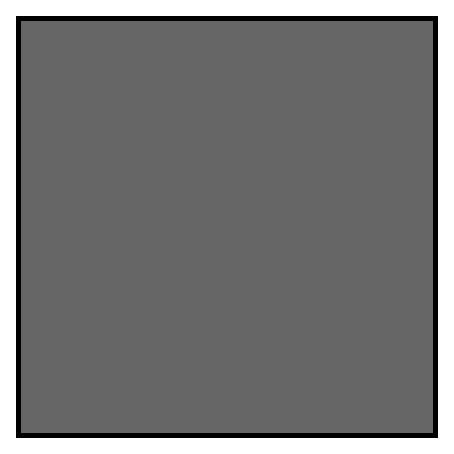
\includegraphics{example.eps}
%}
%% If not, use
%%\vspace{5cm}       % Give the correct figure height in cm
%\caption{Please write your figure caption here}
%\label{fig:1}       % Give a unique label
%\end{figure}
%%
%% For two-column wide figures use
%\begin{figure*}
%% Use the relevant command for your figure-insertion program
%% to insert the figure file. See example above.
%% If not, use
%\vspace*{5cm}       % Give the correct figure height in cm
%\caption{Please write your figure caption here}
%\label{fig:2}       % Give a unique label
%\end{figure*}
%%
%% For tables use
%\begin{table}
%\caption{Please write your table caption here}
%\label{tab:1}       % Give a unique label
%% For LaTeX tables use
%\begin{tabular}{lll}
%\hline\noalign{\smallskip}
%first & second & third  \\
%\noalign{\smallskip}\hline\noalign{\smallskip}
%number & number & number \\
%number & number & number \\
%\noalign{\smallskip}\hline
%\end{tabular}
%% Or use
%\vspace*{5cm}  % with the correct table height
%\end{table}
%%
%% BibTeX users please use
%% \bibliographystyle{}
%% \bibliography{}
%%
%% Non-BibTeX users please use
%\begin{thebibliography}{}
%%
%% and use \bibitem to create references.
%%
%\bibitem{RefJ}
%% Format for Journal Reference
%Author, Journal \textbf{Volume,} (year) page numbers.
%% Format for books
%\bibitem{RefB}
%Author, \textit{Book title} (Publisher, place year) page numbers
%% etc
%\end{thebibliography}

\bibliographystyle{IEEETran}
\bibliography{references}

\end{document}

% end of file template.tex

